\documentclass{wmnotes}

\lecture{Diskrete Mathematik}
\professor{Prof. Stefan Wolf}
\semester{HS 2010}
\author{Michal Sudwoj}
\authoremail{msudwoj@studnet.ethz.ch}
\editor{Simon Etter}
\editoremail{ettersi@student.ethz.ch}

\begin{document}

\part{Vorlesungsnotizen}
\section{Inhalt der Vorlesung}
\begin{itemize}
	\item Logik: Aussagenlogik , Beweise
	\item Mengenlehre: Alle Objekte
	\item Kombinatorik
	\item Graphentheorie
	\item Zahlentheorie, Algebra
	\begin{itemize}
		\item Anwendungen: Kommunikation, Kryptologie, Fehlerkorrektur
	\end{itemize}
\end{itemize}

\chapter{Motivation}
\subsubsection{Worum geht es in dieser Vorlesung?}

\begin{bsp}[note = Modellierung]
\colorbox{White}{\parbox{3\skak}{
	\WhiteKnightOnBlack\WhiteEmptySquare\WhiteKnightOnBlack\\
	\WhiteEmptySquare\BlackEmptySquare\WhiteEmptySquare\\
	\BlackKnightOnBlack\WhiteEmptySquare\BlackKnightOnBlack
}} $\longrightarrow$
\colorbox{White}{\parbox{3\skak}{
	\WhiteKnightOnBlack\WhiteEmptySquare\BlackKnightOnBlack\\
	\WhiteEmptySquare\BlackEmptySquare\WhiteEmptySquare\\
	\BlackKnightOnBlack\WhiteEmptySquare\WhiteKnightOnBlack
}}\\
BILD \\
Fazit: \\
\begin{itemize}
	\item Wegschälen vom Umweltlichen hat das Problem einfach gemacht $\implies$ \textbf{Abbstraktion}
	\item Viele diskrete Probleme führen auf Graphen
\end{itemize}
\end{bsp}

\begin{bsp}[note = Zahlentheorie]
	\begin{gather*}
		N = \{ 0 , 1 , 2 , 3 , \ldots \} \\
 		a \mid b \qquad \text{''a teil b''} \qquad a , b \in \mathbb{N} \\
		a \mid b :\leftrightarrow \exists n \in \mathbb{N} : a \cdot n = b
	\end{gather*}

	\begin{bsp*}
		\begin{gather*}
			2 \mid 6 \\
			3 \nmid 6 \\
			2 \equiv 5 \pmod 3 \\
			3 \not\equiv 5 \pmod 3
		\end{gather*}
	\end{bsp*}
	\begin{equation*}
		\text{p Primzahl} :\leftrightarrow ( a \mid p \rightarrow ( a = 1 \vee a = p ) \wedge p \neq 1 )
	\end{equation*}
	\textbf{Intuition} $\leftrightarrow$ \textbf{Beweis}

	Jede Zahl hat eine \textbf{eindeutige} Primzahlzerlegung (nämlich: \[ p \mid (a \cdot b) \rightarrow p \mid a \vee p \mid b \quad ; \] wir haben's noch nicht bewiesen) \\
	\begin{satz*}
		Es gibt unendlich viele Primzahlen
		\begin{bew}[note = Euklid]
			Annahme: Es gibt nur endlich viele Primzahlen $p_1 , \ldots , p_n$
			\begin{gather*}
				M = p_1 \cdot p_2 \cdot \dotsm \cdot p_n + 1 \\
				\forall i : p_i \nmid M \\
				\text{\lightning} \: \blacksquare
			\end{gather*}
		\end{bew}
	\end{satz*}
\end{bsp}

\begin{bsp}[note = Kombinatorik (''systematisches Zählen'')]
	Kette mit $p$ Perlen in $a$ verschiedene Farben \\
	Anzahl mögliche Ketten? $a^n$ \\
	Anzahl Muster? \\
	Wie oft kommt jedes Muster vor? \\
	Gegeben: $p$ ist prim \\
	\begin{tabular}{ l l }
	$\implies$ einfärbig:		& 1 mal \\
	$\implies$ mehrfärbig:	& p mal
	\end{tabular}
	\begin{gather*}
		\implies \frac{a^p - a}{p} + a = a \cdot ( 1 + \frac{a^{p-1} - 1}{p} ) \\
		a \text{ beliebig}, p \text{ Primzahl} \\
		p \mid ( a^p - a ) \\
		a^p \equiv a \pmod p \\
		( p \nmid a ) \rightarrow ( a^{p-1} \equiv 1 \pmod p ) \\
		\textbf{Kleines Satz von Fermat}
	\end{gather*}
\end{bsp}

\begin{bsp}[note = Geometrie]
	Rechteckige Terrase $a \cdot b \mid a,b \in \mathbb{N}$ \\
	Was sind die grösstmöglichen Quadratplatten, mit denen mann sie exakt belegen kann? \\
	$a \geq b$ \quad Quardat aufteilen in $b \cdot b$ und $(a-b) \cdot b$ \\
	Beobachtungen:
	\begin{itemize}
		\item Jede Belegung des ganzen führt auf separate Belegungen von \\$[b \cdot b]$ und $[(a-b) \cdot b]$
		\item Es reicht, $[(a-b) \cdot b]$ zu berechnen.
	\end{itemize}
	$$\mathrm{R}_{a-b}(b) = b \bmod (a-b)$$
	Fortfahren, bis wir ein Quadrat erhalten. Warum wird das sicher passieren? \\
	\quad Spätestens bei $1 \cdot 1$\\
	Algorithmus (Euklid):
	\begin{gather*}
		a , b \\
		r_1 = \mathrm{R}_b(a) \\
		r_2 = \mathrm{R}_{r_1}(b) \\
		\vdots \\
		r_n = \mathrm{R}_{r_{n-1}}(r_{n-2}) \\
		\vdots \\
		r_k = \ggt(a,b) \\
		0
	\end{gather*}
\end{bsp}

\begin{bsp}
	2 Sanuhren: 21 min und 15 min. Wir wollen 3 min abmessen. \\
	\begin{tabular}{ c c c c c c }
		Euklid:	& 21,	& 15,	& 6,	& 3,	& 0 \\
		21 min:	& 1	&0	&1	&-2 \\
		15 min:	&0	&1	& -1	&3
	\end{tabular}
\end{bsp}

\begin{bsp}[note = Verbindungen ohne Überkreuzen]
	3 Häuser mit 3 Werke verbinden $\rightarrow$ geht nicht! \\
	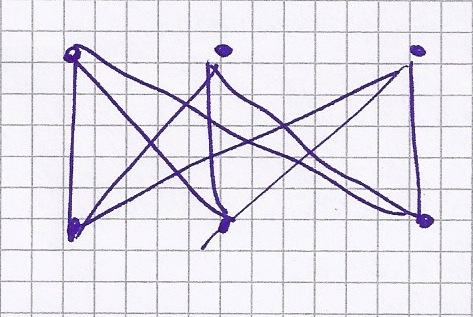
\includegraphics{Bild2} \\
	der Graph ist nicht \textbf{planar}. \\
	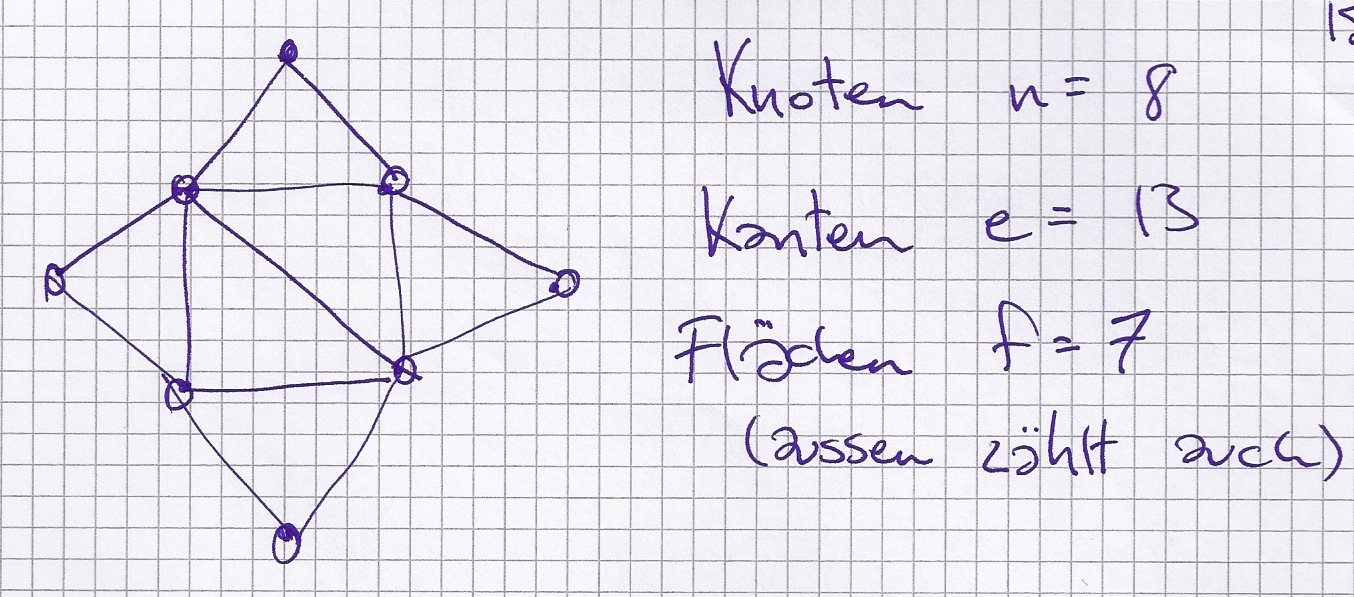
\includegraphics[width=\textwidth]{Bild3}
	\begin{bew}[head = Beweisidee:]
		\quad Für einen Baum (kreislos, zusammenhängend) gilt $n = e +1 \implies n - e + f = 2$ \\
		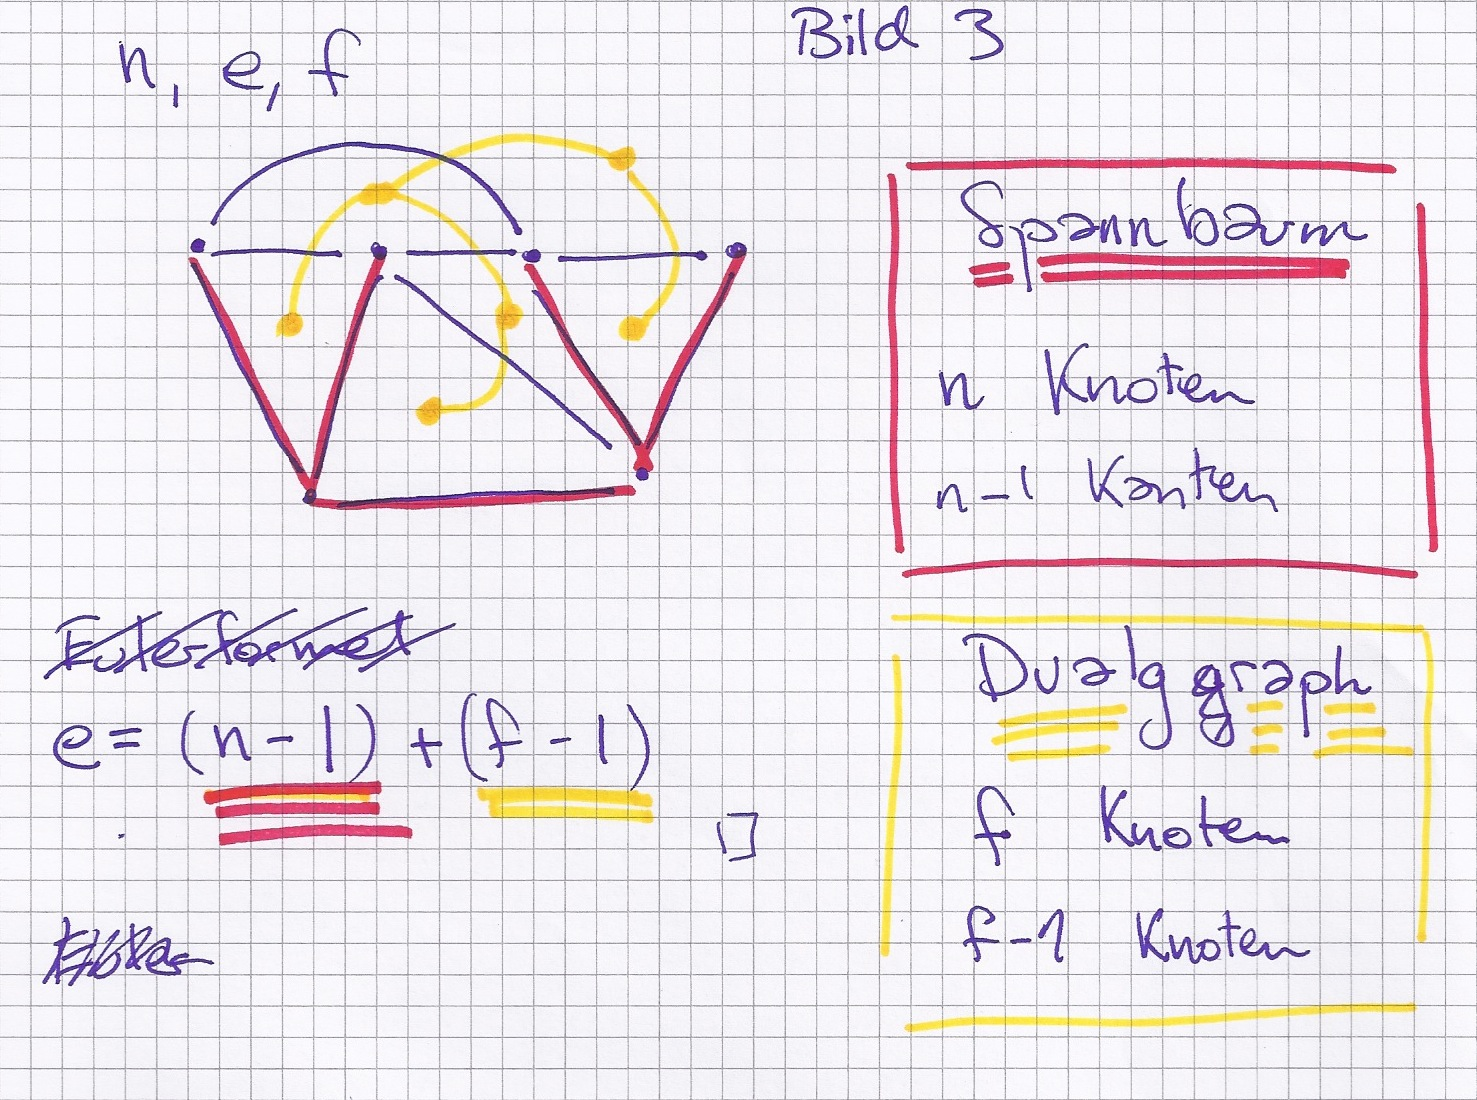
\includegraphics[width=\textwidth]{Bild4} \\
		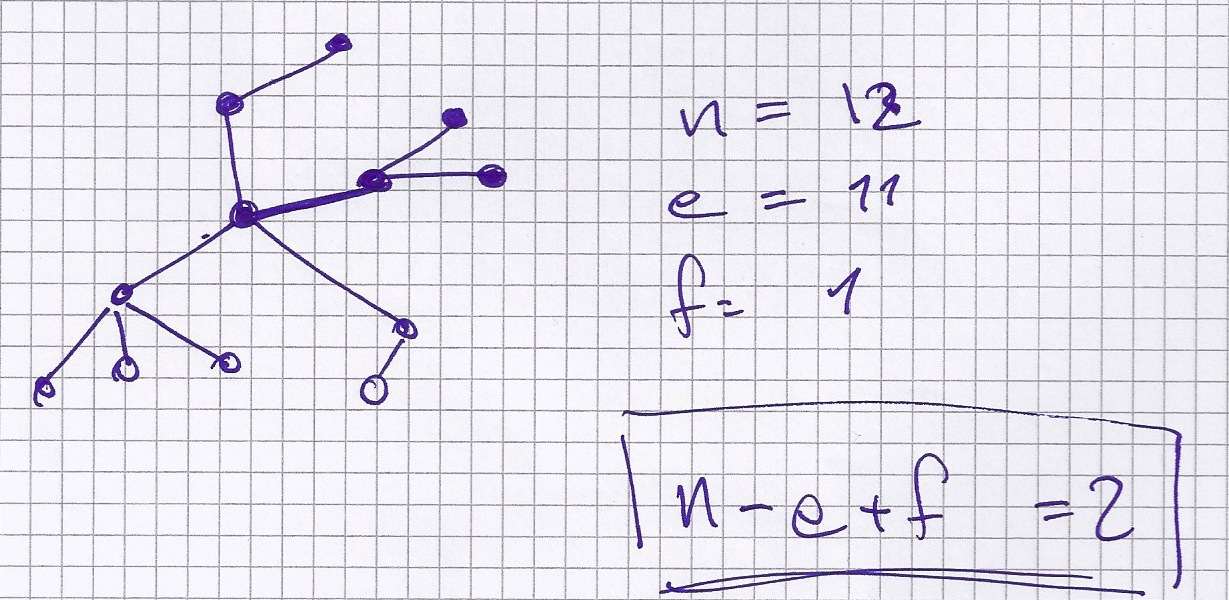
\includegraphics[width=\textwidth]{Bild5} \\
		\textbf{Eulersche Polyederformel}
	\end{bew}
\end{bsp}

\chapter{Logik}
\section{Was ist Logik?}
\textit{\enquote{Septem artes liberalen}}, 7 freie Künste \\
Fächerkanon:
\begin{itemize}
	\item Trivium
	\begin{itemize}
		\item Grammatik
		\item Rhetorik
		\item Logik
	\end{itemize}
	\item Quadrivium
	\begin{itemize}
		\item Arithmetik
		\item Geometrie
		\item Musik
		\item Astronomie
	\end{itemize}
\end{itemize}
$\drsh$ \enquote{trivial} \\
\enquote{logos}: argumentierende, begründende Rede, vernünftiges Sprechen \\
Logik: Lehre des Begründens, Argumentierens, Schliessens \\
\begin{tabular}{lll}
	1918:	& Frege:	& $\frac{\text{schön}}{\text{Ästhetik}} = \frac{\text{gut}}{\text{Ethik}} = \frac{\text{wahr}}{\text{Logik}}$ \\
	1970:	& Patzig:	& Logik = Theorie der Aussagen, die aufgrund \textbf{ihrer Form} wahr sind. \\
	1985:	& Menne:	& Logik = Lehre von der \textbf{Folgerichtigkeit}
\end{tabular}
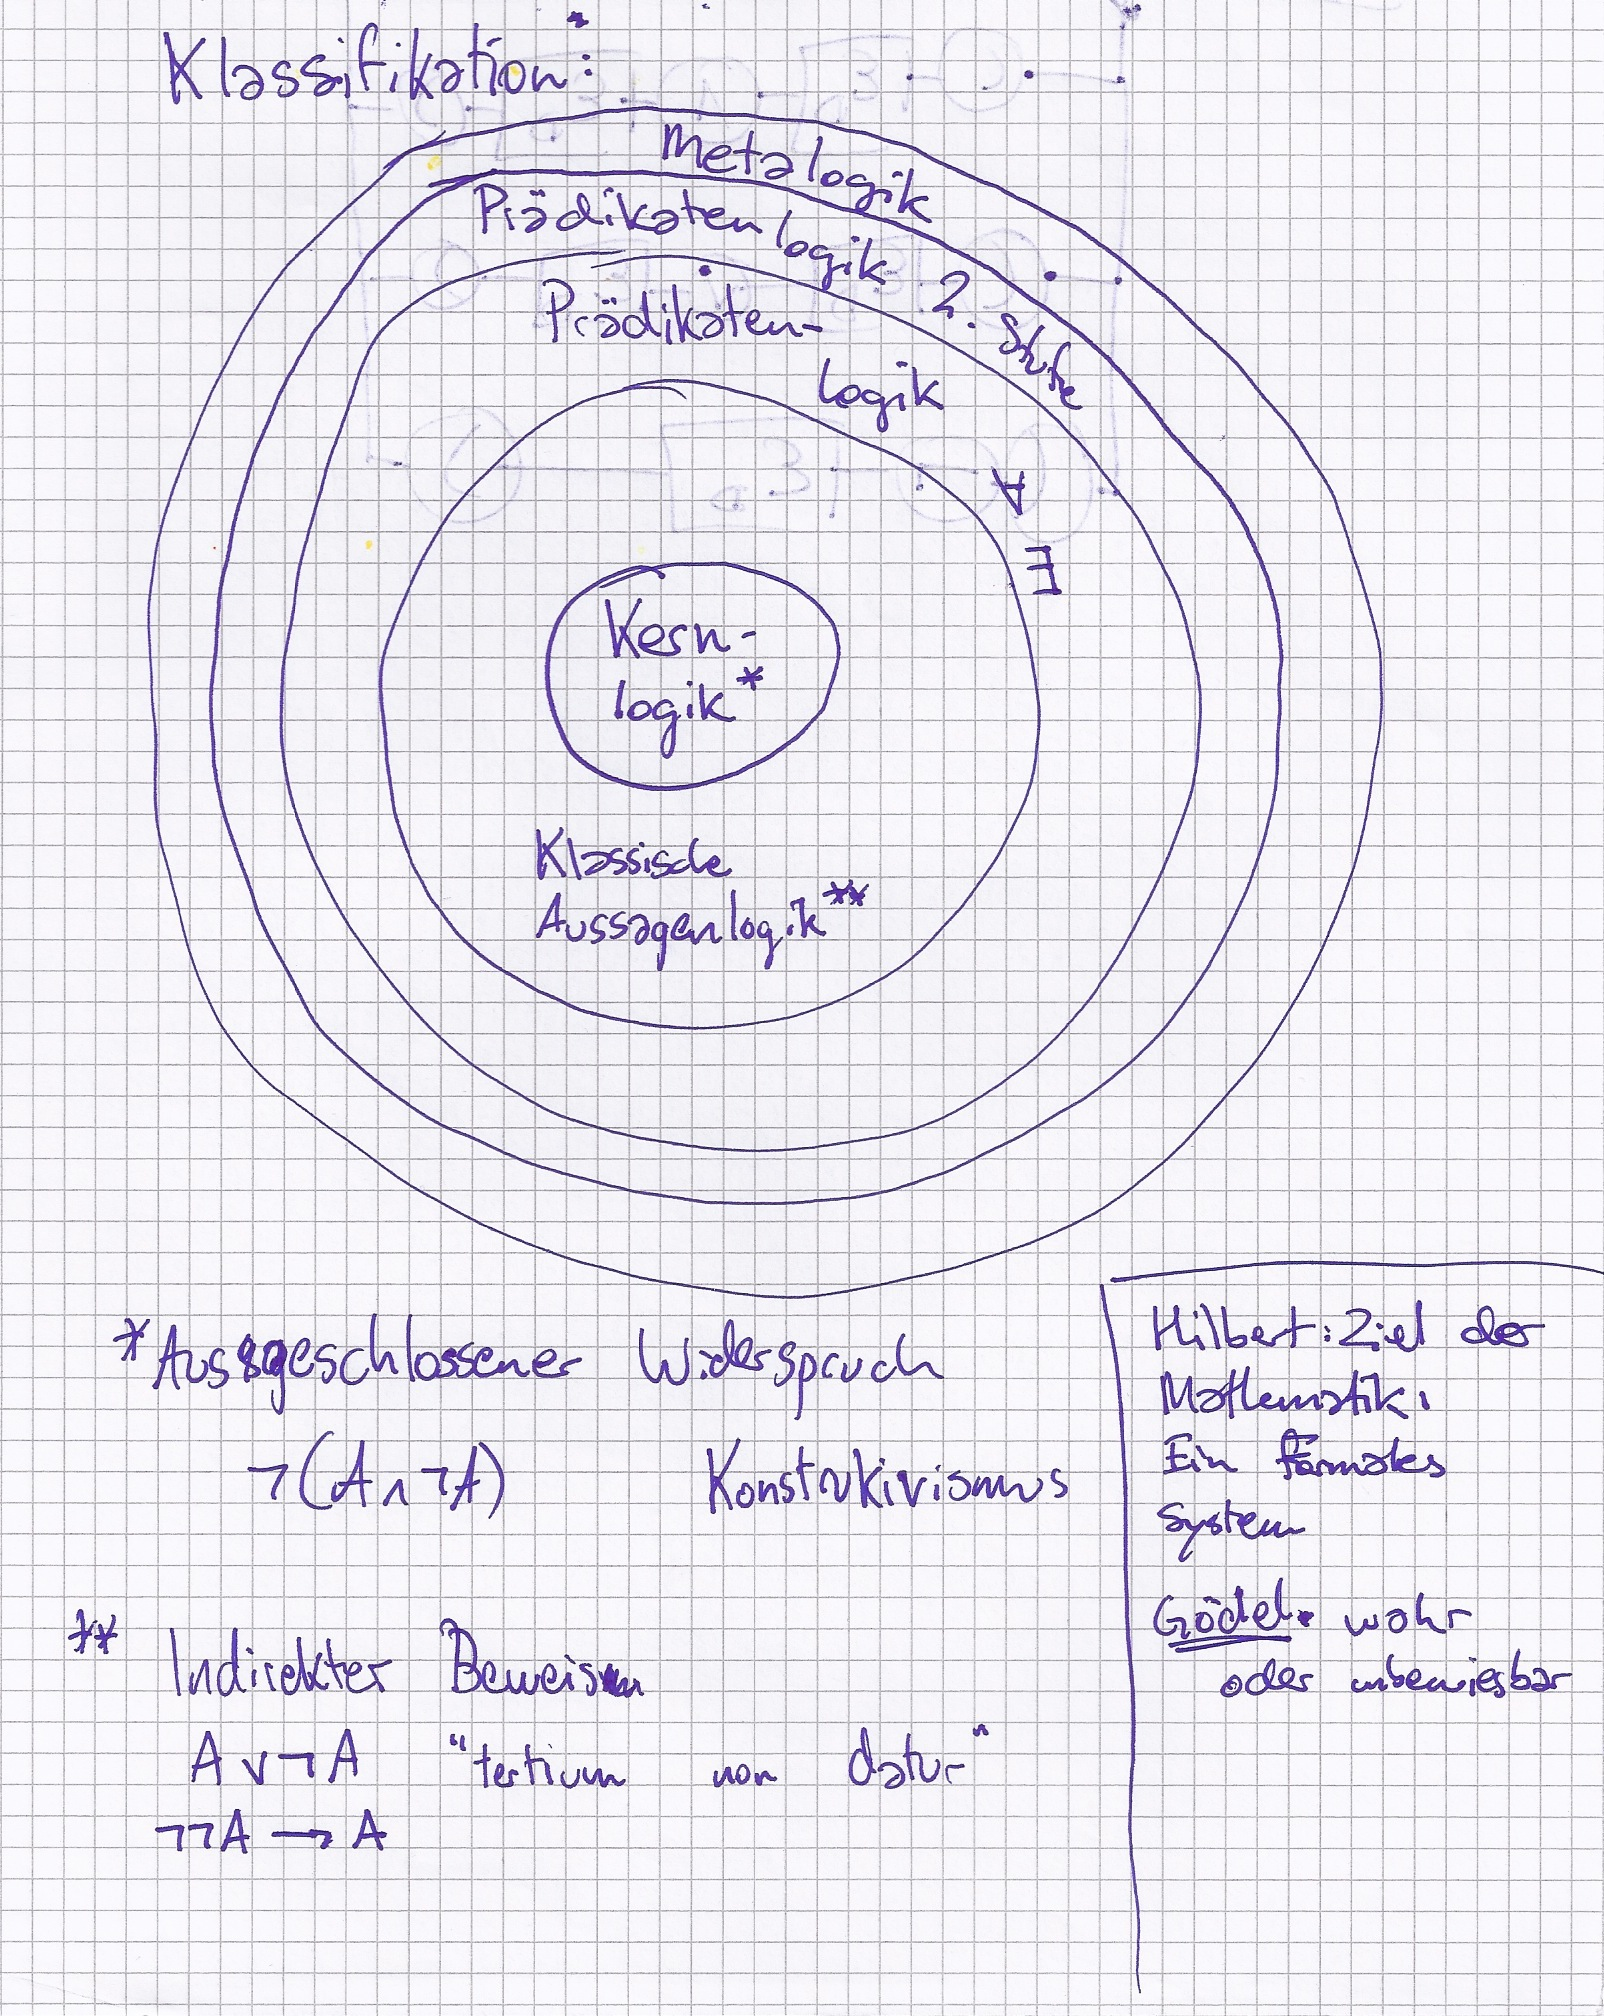
\includegraphics[width=\textwidth]{Bild6} \\
\begin{bsp*}
	Gibt es $r_1 , r_2 \notin \Q \text{ mit } {r_1}^{r_2} \in \Q$ ? Ja.
	\begin{gather*}
		\sqrt{2} \notin \Q \qquad
		\begin{bmatrix*}{l}
			\sqrt{2} = \frac{p}{q} \rightarrow 2p^2 = q^2 \rightarrow p = 2p' \rightarrow 2p^2 = 4{p'}^2 \\
			\implies \text{Bruch nicht gekürzt.}
		\end{bmatrix*} \\
		{\sqrt{2}}^{\sqrt{2}} \in \Q \vee {\sqrt{2}}^{\sqrt{2}} \notin \Q \qquad \sqrt{2}^{{\sqrt{2}}^{\sqrt{2}}} = 2
	\end{gather*}
\end{bsp*}

\section{Aussagenlogik}
\subsection{Definitionen}
\begin{def*}[note = Aussage , index = Aussage]
	\textbf{Eine Aussage ist ein sprachlicher Ausdruck, der wahr oder falsch ist.}
\end{def*}
\begin{bsp*}
	\begin{itemize}
		\item Wenn es regnet, dann sind die Strassen nass.
		\item Wenn der Hahn kräht auf dem Mist, ändert das Wetter oder es bleibt wie es ist.     (Tautologie)
		\item Dies ist keine Aussage. \qquad (Aussage, falsch)
		\item Diese Aussage ist falsch.
		\item Wale sind Fische und Fische sind Tiere.
	\end{itemize}
\end{bsp*}
\textbf{Atomare Aussagen} mit \textbf{Junktoren} verbunden $\rightarrow$ Zusammengesetzte Aussagen.

\subsubsection{Junktoren als Wahrheitsfunktionen}
\qquad $\drsh$ Wahrheitstabellen \\
\url{http://en.wikipedia.org/wiki/Logical_connective} \\
AND (konjunktion) \\
\begin{tabular}{ | l | l | l | }
	\hline
	$A$	& $B$	& $A \wedge B$	\\ \hline
	W	& W		& W			\\ \hline
	W	& F		& F			\\ \hline
	F	& W		& F			\\ \hline
	F	& F		& F			\\ \hline
\end{tabular} \\
NOT \\
\begin{tabular}{ | l | l | }
	\hline
	$A$	& $\neg A$	\\ \hline
	W	& F			\\ \hline
	W	& F			\\ \hline
\end{tabular} \\
NAND (universell) \\
\begin{tabular}{ | l | l | l | }
	\hline
	$A$	& $B$	& $A \mid B$	\\ \hline
	W	& W		& F			\\ \hline
	W	& F		& W			\\ \hline
	F	& W		& W			\\ \hline
	F	& F		& W			\\ \hline
\end{tabular}\\
OR (disjunktion) \\
\begin{tabular}{ | l | l | l | }
	\hline
	$A$	& $B$	& $A \vee B$	\\ \hline
	W	& W		& W			\\ \hline
	W	& F		& W			\\ \hline
	F	& W		& W			\\ \hline
	F	& F		& F			\\ \hline
\end{tabular} \\
XOR (ausschliessendes Oder) \\
\begin{tabular}{ | l | l | l | }
	\hline
	$A$	& $B$	& $A \oplus B$	\\ \hline
	W	& W		& F			\\ \hline
	W	& F		& W			\\ \hline
	F	& W		& W			\\ \hline
	F	& F		& F			\\ \hline
\end{tabular} \\
XNOR (Äquivalenz) \\
\begin{tabular}{ | l | l | l | }
	\hline
	$A$	& $B$	& $A \leftrightarrow B$	\\ \hline
	W	& W		& W					\\ \hline
	W	& F		& F					\\ \hline
	F	& W		& F					\\ \hline
	F	& F		& W					\\ \hline
\end{tabular} \\
$A \leftrightarrow B \equiv \neg ( A \oplus B )$ \\
Implikation \\
\begin{tabular}{ | l | l | l | }
	\hline
	$A$	& $B$	& $A \rightarrow B$	\\ \hline
	W	& W		& W			\\ \hline
	W	& F		& F			\\ \hline
	F	& W		& W			\\ \hline
	F	& F		& W			\\ \hline
\end{tabular} \\
$A \rightarrow B \equiv ( \neg A ) \vee B$ \\
\begin{bem}
	$A \rightarrow B$ ist nicht gleich $ B \rightarrow A$ oder $\neg A \rightarrow \neg B$
\end{bem}
\begin{gather*}
	A \rightarrow B \equiv \neg B \rightarrow \neg A \qquad \text{(indirekter Beweis)} \\
	B \rightarrow A \equiv \neg A \rightarrow \neg B
\end{gather*}
\subsubsection{Syntax \texorpdfstring{$\leftrightarrow$}{<->} Semantik}
\begin{tabular}{ l l }
	Syntax:	& Welche Zeichenketten sind korrekte Formeln? \\
	Semantik:	& Für korrekte Formeln: wahr oder falsch?
\end{tabular}

\subsection{Syntax der Aussagenlogik}
\begin{def*}[note = korrekte Formel , index = Formel!korrekte]
	Syntaktisch korrekte Formel $\epsilon_D$ über Atomformeln $D \coloneqq \{ A , B , C , \dotsc , A_1 , B_1 , \dotsc \}$ \\
	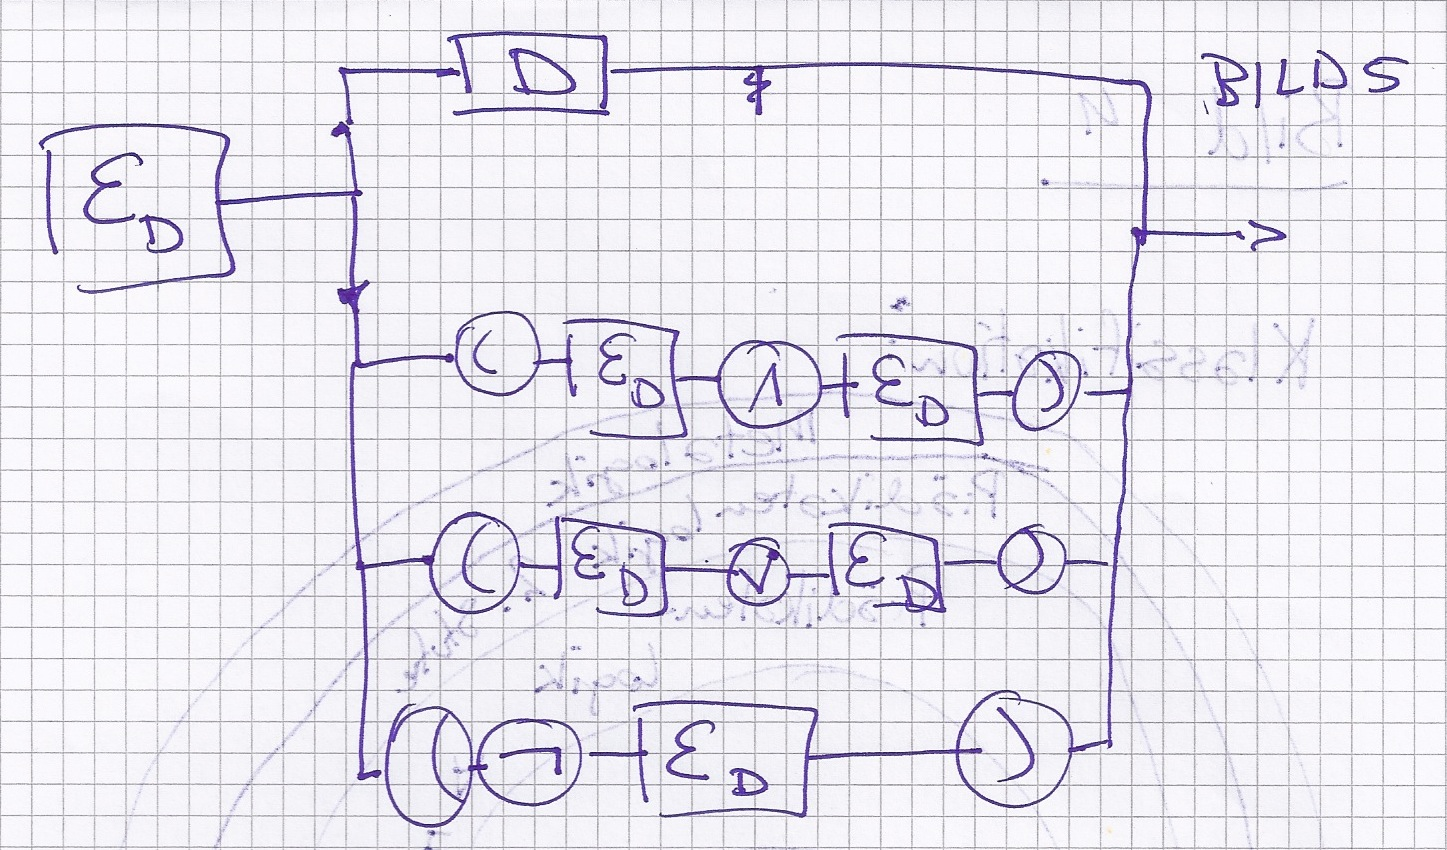
\includegraphics[width=\textwidth]{Bild7} \\
	Syntaktisch korrekte Formeln $\epsilon_D$ ist definiert über Atomformeln $D$:
	\begin{itemize}
		\item Atomformeln
		\item Falls $f$ und $g$ syntaktisch korrekt, dann auch $( \neg f ) , ( f \wedge g ) , ( f \vee g )$
		\item Das ist alles.
	\end{itemize}
\end{def*}
\begin{bsp*}
	\begin{itemize}
		\item $A$
		\item $( \neg A )$
		\item $( \neg ( \neg A ) )$
		\item $B$
		\item $( A \wedge B )$
		\item $( A \wedge A )$
		\item $( ( ( A \wedge B ) \vee ( \neg C ) ) \wedge ( A \vee B ) )$
	\end{itemize}
\end{bsp*}
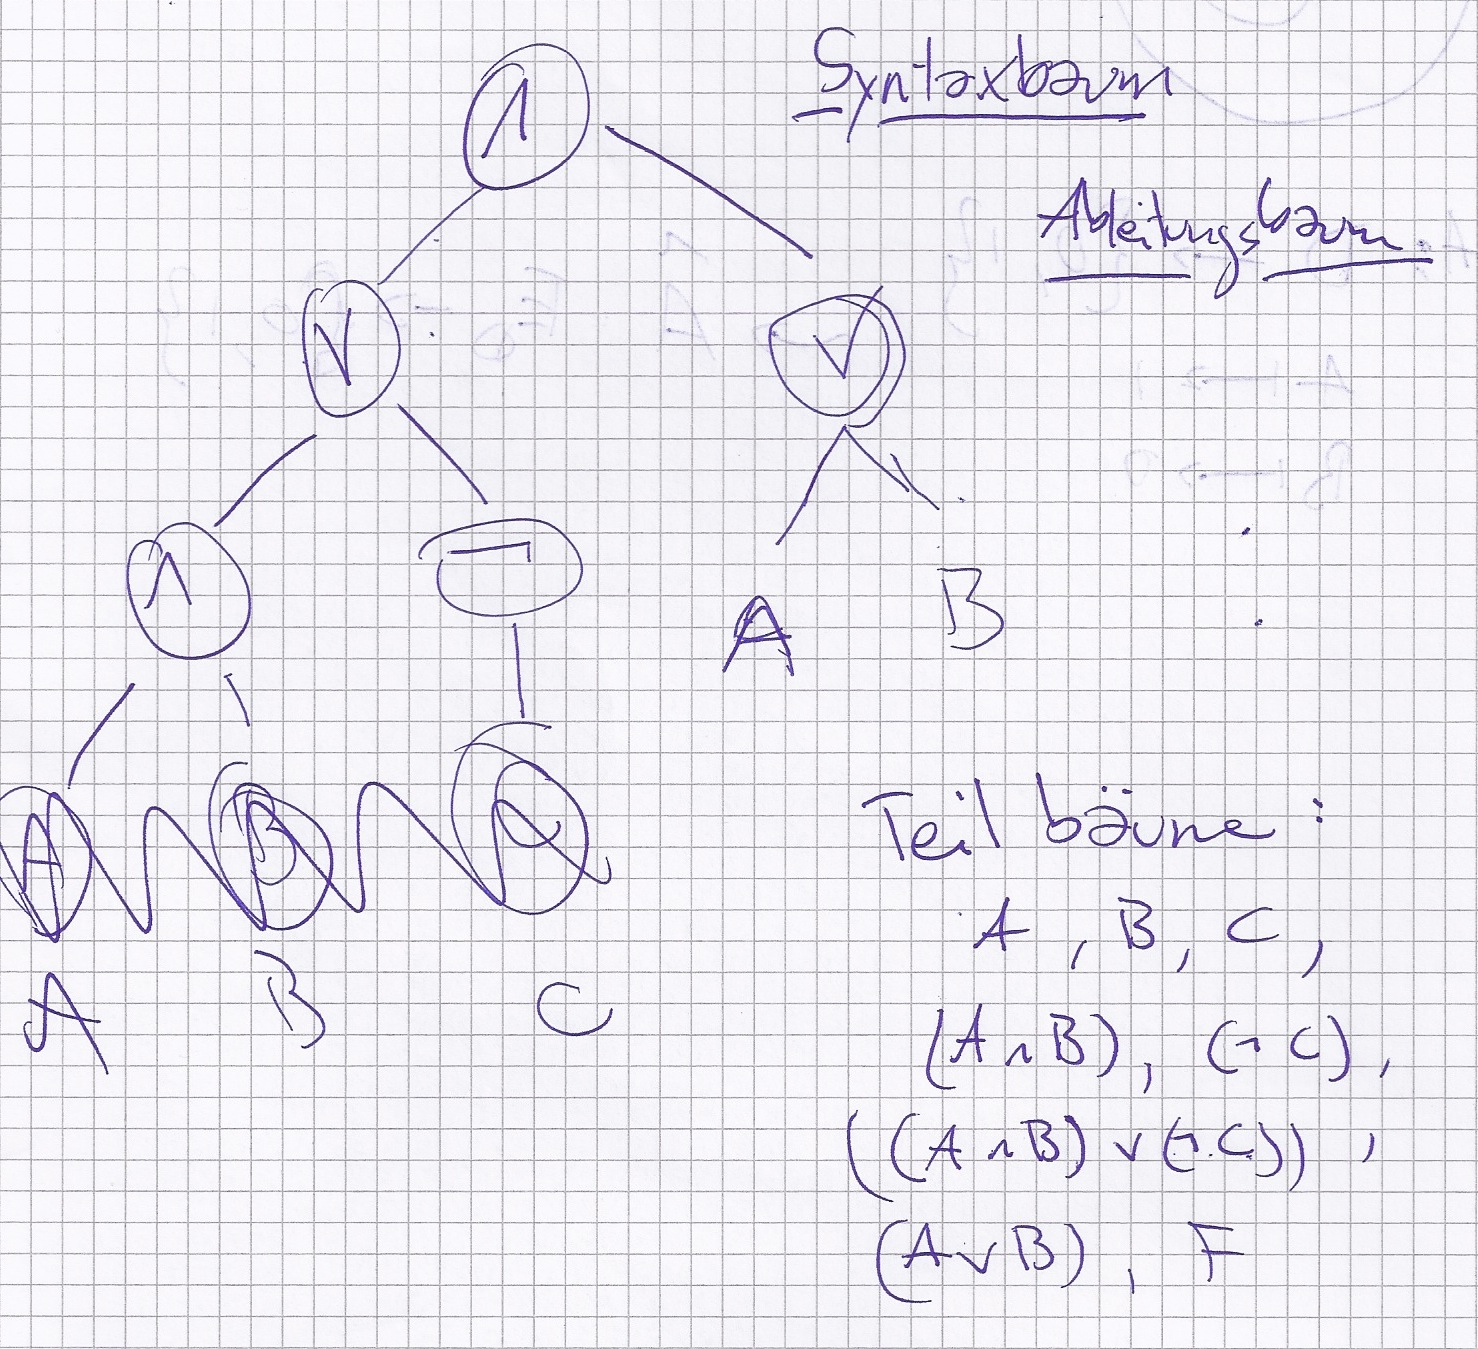
\includegraphics[width=\textwidth]{Bild8} \\
Teilformel = Teilstring, der selbst eine Formel ist. \\
\begin{bsp*}
	\begin{itemize}
		\item $A$
		\item $B$
		\item $C$
		\item $( A \wedge B )$
		\item $( \neg C )$
		\item $( ( A \wedge B ) \vee ( \neg C ) )$
		\item $( A \vee B )$
		\item $F$
	\end{itemize}
\end{bsp*}

\subsection{Semantik der Aussagenlogik}
Wahrheitswerte der Atomformeln $\rightarrow$ Wahrheitswerte der zusammengesetzten Formeln
\subsubsection{Vollständige Wahrheitstabelle}
$((( A \wedge B ) \vee ( \neg C )) \wedge ( A \vee B ))$
\begin{gather*}
	\begin{array}{ c c c c c c c c c c >{\columncolor{green}}c c c c c c }
		(((	& A	& \wedge	& B	& )	& \vee	& (	& \neg	& C	& ))	& \wedge	& (	& A	& \vee	& B	& ))	\\
			& 0	& 0		& 0	&	& 1		&	& 1		& 0	&	& 0		&	& 0	& 0		& 0		\\
			& 0	& 0		& 0	&	& 0		&	& 0		& 1	&	& 0		&	& 0	& 0		& 0		\\
			& 0	& 0		& 1	&	& 1		&	& 1		& 0	&	& 1		&	& 0	& 1		& 1		\\
			& 0	& 0		& 1	&	& 0		&	& 0		& 1	&	& 0		&	& 0	& 1		& 1		\\
			& 1	& 0		& 0	&	& 1		&	& 1		& 0	&	& 1		&	& 1	& 1		& 0		\\
			& 1	& 0		& 0	&	& 0		&	& 0		& 1	&	& 0		&	& 1	& 1		& 0		\\
			& 1	& 1		& 1	&	& 1		&	& 1		& 0	&	& 1		&	& 1	& 1		& 1		\\
			& 1	& 1		& 1	&	& 1		&	& 0		& 1	&	& 1		&	& 1	& 1		& 1		
	\end{array}
\end{gather*}
\begin{def*}[note = Belegung , index = Belegung]
	D , $\epsilon_D$ \hyperref[Formel!korrekte]{wie oben}. \\
	\begin{gather*}
		\begin{array}{ l l }
			\mathcal{A} : D \rightarrow \{ 0 , 1 \}				& \text{Belegung} \\
			\mathcal{\hat{A}} : \varepsilon_D \rightarrow \{ 0 , 1 \}	& \text{Fortsetzung von } \mathcal{A}
		\end{array}
	\end{gather*}
	\begin{itemize}
		\item $\mathcal{\hat{A}}( D ) \coloneqq \mathcal{A}( D ) \qquad \text{für Atomformel D}$
		\item $\mathcal{\hat{A}}(( F \wedge G )) \coloneqq \mathcal{\hat{A}}( F ) \wedge \mathcal{\hat{A}}( G )$
		\item $\mathcal{\hat{A}}(( F \vee G )) \coloneqq \mathcal{\hat{A}}( F ) \vee \mathcal{\hat{A}}( G )$
		\item $\mathcal{\hat{A}}(( \neg F )) \coloneqq 1 - \mathcal{\hat{A}}( F )$
	\end{itemize}
\end{def*}

\subsubsection{Vereinfachungen:}
\begin{itemize}
	\item Weglassen von Klammern
	\item Andere Junktoren ( als Abkürzungen )
\end{itemize}
\subsubsection{Semantische Äquivalenz}
\begin{gather*}
	\begin{array}{ c c c c c c c >{\columncolor{green}}c c c c c c }
		((	& \neg	& (	& A	& \wedge	& B	& ))	& \wedge	& (	& A	& \vee	& B	& ))	\\
			& 1		&	& 0	& 0		& 0	&	& 0		&	& 0	& 0		& 0		\\
			& 1		&	& 0	& 0		& 1	&	& 1		&	& 0	& 1		& 1		\\
			& 1		&	& 1	& 0		& 0	&	& 1		&	& 1	& 1		& 0		\\
			& 0		&	& 1	& 0		& 1	&	& 0		&	& 1	& 1		& 1					
	\end{array}\\
	\intertext{Diese beiden Formel sind syntaktisch verschieden, aber semantisch äquivalent (logisch gleichwertig).}
	\begin{array}{ c >{\columncolor{green}}c c }
		A	& \oplus	& B	\\
		0	& 0		& 0	\\
		0	& 1		& 1	\\
		1	& 0		& 0	\\
		1	& 0		& 1	
	\end{array}\\
	A \oplus B \equiv (( \neg ( A \wedge B ) \wedge ( B \vee A )) \equiv ((( \neg A ) \wedge B ) \vee ( A \wedge ( \neg B )))
\end{gather*}
\begin{def*}[note = {semantische Äquivalenz, Tautologie, Unerfüllbarkeit} , index = Semantik!Äquivalenz]
	Formeln F und G sind semantisch äquivalent, falls sie für jede Belegung den gleichen Wahrheitswert haben. \\
 	Wir schreiben $F \equiv G$ oder $F \iff G$. \\
	\begin{gather*}
		0 \coloneqq ( A \wedge ( \neg A ) ) \\
		1 \coloneqq ( A \vee ( \neg A ) )
	\end{gather*}
	Eine Formel $F \equiv 1$ heisst \textbf{Tautologie}\index{Formel!Tautologie}.\\
	Eine Formel $F \equiv 0$ heisst \textbf{unerfüllbar}\index{Formel!unerfüllbar}.
\end{def*}
\begin{satz*}
	$F \equiv G$ gilt \gdw $F \leftrightarrow G$ eine Tautologie ist. \\
	$( F \leftrightarrow G \coloneqq ( ( F \wedge G ) \vee ( ( \neg F ) \wedge ( \neg G ) )$ \\
	\begin{bew}
		$F \equiv G$ : Für jede Belegung haben $F$ und $G$ den gleichen Wahrheitswert.\\
		Gleichbedeutend mit: Für jede Belegung ist $F \leftrightarrow G$ wahr.
	\end{bew}
\end{satz*}
\begin{bsp*}[note = Äquivalenzen, index = logische Gesetze]
	\begin{gather*}
		\begin{array}{ l l l }
			\text{Idempotenz:}		& ( F \wedge F )				&\equiv F							\\
								& ( F \vee F )				&\equiv F							\\
			\text{Kommutativität:}		& ( F \wedge G )				&\equiv ( G \wedge F )					\\
								& ( F \vee G )				&\equiv ( G \vee F )					\\
			\text{Assoziativität:}		& ( ( F \wedge G  ) \wedge H )	&\equiv ( F \wedge ( G  \wedge H ) )		\\
								& ( ( F \vee G  ) \vee H )		&\equiv ( F \vee ( G  \vee H ) )			\\
			\text{Distibutivität:}		& ( F \wedge ( G  \vee H ) )		&\equiv ( ( F \wedge G ) \vee ( F \wedge H ) )	\\
								& ( F \vee ( G  \wedge H ) )		&\equiv ( ( F \vee G ) \wedge ( F \vee H ) )	\\
			\text{de Morgan:}		& ( \neg ( F \wedge G ) )		&\equiv( ( \neg F ) \vee ( \neg G ) )		\\
								& ( \neg ( F \vee G ) )			&\equiv( ( \neg F ) \wedge ( \neg G ) )		\\
			\text{Doppelte Negation:}	& ( \neg ( \neg F ) )			&\equiv F							
		\end{array}
	\end{gather*}
\end{bsp*}

\subsubsection{Vereinfachungen:}
\begin{itemize}
	\item $A \rightarrow B \text{ für } ( ( \neg A ) \vee B )$
	\item $A \oplus B , A \leftrightarrow B$
	\item $A \wedge B \wedge C$
	\item Priorität (absteigend):
	\begin{itemize}
		\item $\neg$
		\item $\wedge , \vee$
		\item $\leftarrow , \leftrightarrow$
	\end{itemize}
\end{itemize}
Formel $F$ in $A_1 , \dotsc , A_n$ entspricht einer Funktion:\\
Belegung $\mapsto$ Auswertung\\
$\{ 0 , 1 \} \rightarrow \{ 0 , 1 \}$

\subsubsection{Berechnung und Auswertung in Wahrheitstabellen}
\begin{gather*}
	\begin{array}{ c c c c c c >{\columncolor{green}}c c }
		(	& \neg	& A_1	& \oplus	& A_2	& )	& \rightarrow	& A_3	\\
			& 1		& 0		& 1		& 0		&	& 0			& 0		\\
			& 1		& 0		& 1		& 0		&	& 1			& 1		\\
			& 1		& 0		& 0		& 1		&	& 1			& 0		\\
			& 1		& 0		& 0		& 1		&	& 1			& 1		\\
			& 0		& 1		& 0		& 0		&	& 1			& 0		\\
			& 0		& 1		& 0		& 0		&	& 1			& 1		\\
			& 0		& 1		& 1		& 1		&	& 0			& 0		\\
			& 0		& 1		& 1		& 1		&	& 1			& 1		
	\end{array}
\end{gather*}\\
Formeln mit gleicher Funktionen sind \enquote{semantisch Äquivalent}.

\subsubsection{Normalformen}
Formel $\rightarrow$ Wahrheitsfunktion \\
Formel $\leftarrow$ Wahrheitsfunktion ? \\
\begin{gather*}
	\begin{array}{ c c c >{\columncolor{green}}c }
		A 	& B	& C	& F	\\
		0	& 0	& 0	& 0	\\
		0	& 0	& 1	& 0	\\
		0	& 1	& 0	& 1	\\
		0	& 1	& 1	& 1	\\
		1	& 0	& 0	& 1	\\
		1	& 0	& 1	& 1	\\
		1	& 1	& 0	& 0	\\
		1	& 1	& 1	& 1	\\
	\end{array}\\
	\begin{array}{ l l }
	F 	& \equiv ( \neg A \wedge B \wedge \neg C ) \vee ( \neg A \wedge B \wedge C ) \vee ( A \wedge \neg B \wedge \neg C ) \vee ( A \wedge  \neg B \wedge C ) \vee ( A \wedge B \wedge C ) \\
		& \equiv ( ( \neg A \wedge B ) \wedge ( C \vee \neg C ) ) \vee ( ( A \vee \neg B ) \wedge ( C \vee \neg C ) ) \vee ( A \wedge B \wedge C ) \\
		& \equiv ( \neg A \wedge B ) \vee ( A \wedge \neg B ) \vee ( A \wedge B \wedge C )
	\end{array}\\
	\textbf{ Disjunktive Normalform DNF}\\
	\begin{array}{ l l }
		F	& \equiv ( A \vee B \vee C ) \wedge ( A \vee B \vee \neg C ) \wedge ( \neg A \vee \neg B \vee C )	\\
			& \equiv ( ( A \vee B ) \vee ( C \wedge \neg C ) ) \wedge ( \neg A \vee \neg B \vee C )			\\
			& \equiv ( A \vee B ) \wedge ( \neg A \vee \neg B \vee C )							
	\end{array}\\
	\textbf{Konjunktive Normalform KNF}
\end{gather*}\\
\begin{def*}[note = {DNF, KNF} , index = Normalform]
	\begin{itemize}
		\item \textbf{Literal}\index{Literal}: $F$ Atomformel, dann sind $F, \neg F$ Literale.
		\item $F$ in \textbf{KNF}\index{KNF}\index{Normalform!konjunktive}, falls es Literale $L_{ij}$ gibt mit $\bigwedge_{i=1}^k ( \bigvee_{j=1}^{m_i} L_{ij} )$
		\item $F$ in \textbf{DNF}\index{DNF}\index{Normalform!disjunktive}, falls es Literale $L_{ij}$ gibt mit $\bigvee_{i=1}^k ( \bigwedge_{j=1}^{m_i} L_{ij} )$
	\end{itemize}
\end{def*}

\subsubsection{Modell und semantische Folgerung}
\begin{def*}[note = Modell , index = Modell]
	Sei $F$ eine Formel und $\mathcal{A}$ eine Belegung mit $\mathcal{A}( F ) \equiv 1$ . Dann heisst $\mathcal{A}$ ein \textbf{Modell} in $F$, man schreibt $\mathcal{A} \models F$
\end{def*}
\begin{bsp*}
	\begin{gather*}
		\begin{array}{ c c c c c >{\columncolor{green}}c c }
			(	& A	& \wedge	& B	& )	& \rightarrow	& C	\\
				& 0	& 0		& 0	&	& 1			& 0	\\
				& 0	& 0		& 0	&	& 1			& 1	\\
				& 0	& 0		& 1	&	& 1			& 0	\\
				& 0	& 0		& 1	&	& 1			& 1	\\
				& 1	& 0		& 0	&	& 1			& 0	\\
				& 1	& 0		& 0	&	& 1			& 1	\\
				& 1	& 1		& 1	&	& 0			& 0	\\
				& 1	& 1		& 1	&	& 1			& 1	
		\end{array}
	\end{gather*}
	Tatsachen:
	\begin{itemize}
		\item $F \equiv G$ \gdw $( \mathcal{A} \models G \text{ \gdw} \mathcal{A} \models G )$ .
		\item $F$ Tautologie, falls $\mathcal{A} \models F$ für alle $\mathcal{A}$ .
		\item $F$ unerfüllbar, falls $\mathcal{A} \models F$ für kein $\mathcal{A}$ .
	\end{itemize}
\end{bsp*}
\marginpar{\color{red}$\models$ gleich wie $\implies$}
\begin{def*}[note = semantische Folgerung , index = semantische Folgerung]
	\begin{gather*}
		G \text{ ist eine semantische Folgerung von } F_1 , \dotsc , F_n \\
		F_1 , \dotsc , F_n \models G \\
		F_1 , \dotsc , F_n \implies G \\
		\text{falls für alle } \mathcal{A} \text{ mit } \mathcal{A} \models F_1 , \dotsc , \mathcal{A} \models F_n \text{ auch } \mathcal{A} \models G \text{ gilt.}
	\end{gather*}
\end{def*}
\begin{bem}
		$F \equiv G$ gleichbedeutend mit $F \models G$ und $G \models F$ ( Manchmal sieht man $ F \vDash\joinrel\Dashv G$ oder $F \iff G$ )
\end{bem}
\begin{bsp*}
		\begin{gather*}
		A , A \rightarrow B , B \rightarrow C \models C\\
		\begin{split}
			& \text{Die einzige Belegung, die } A , A \rightarrow B \text{ und } B \rightarrow C \text{ erfüllt  } \\
			& \text{ ist die Belegung } A \equiv B \equiv C \equiv 1 \\
		\end{split}\\
		\text{Für jede } \mathcal{A} \text{ die das erfüllt, ist auch } C \text{ erfüllt.} \\
		F \equiv G \text{ \gdw } F \leftrightarrow G \text{ Tautologie} \\
		F \models G \text{ \gdw } F \rightarrow G \text{ Tautologie} \\
		A \wedge ( A \rightarrow B ) \wedge ( B \rightarrow C ) \rightarrow C \text{ Tautologie}
	\end{gather*}
\end{bsp*}
\begin{satz*}
	$F_1 , \dotsc , F_n \models G \text{ \gdw } \bigwedge_{i=0}^n F_i \rightarrow G \text{ Tautologie}$\\
	\begin{bew}
		\[\bigwedge_{i=1}^n F_i \rightarrow G \equiv \neg ( \bigwedge_{i=1}^n F_i  ) \vee G \equiv ( \bigvee_{i=1}^n F_i  ) \vee G\]
	\end{bew}
	Beides gilt \gdw für jede Belegung $\mathbb{A}$ gilt:\\
	\qquad falls $\mathcal{A}( F_i ) = 1$ für alle $i$ dann auch $\mathcal{A}( G ) = 1$
\end{satz*}
\begin{bem}
	\begin{itemize}
		\item $F$ Tautologie \gdw $1 \models F$
		\item $F$ unerfüllbar \gdw $F \models 0$
	\end{itemize}
\end{bem}

\subsection{Beweistheorie der Aussagenlogik}
\subsubsection{Typische Fragestellungen}
\begin{itemize}
	\item Ist $F$ Tautologie?
	\item Ist $G$ erfüllbar? \qquad ( Ist $G$ Tautologie? )
	\item Gilt $A_1 , \dotsc , A_n \models B$ \quad (= Ist $A_1 \wedge \dotsb \wedge A_n \rightarrow B$ Tautologie? = \\
		Ist $A_1 \wedge \dotsb \wedge A_n \wedge B$ unerfüllbar?)
\end{itemize}
\begin{bsp}
	\begin{gather*}
		F = \bigwedge_{i=1}^n ( \bigvee_{j=1}^{m_i} L_{ij} ) \qquad \text{Ist } F \text{ Tautologie?} \\
		F = F_1 \wedge \dotsb \wedge F_n \\
		F \text{ Tautologie, \gdw } F_1 , \dotsc , F_n \text{ Tautologien} \\
		\begin{split}
			& F_1 = L_{1,1} \vee \dotsb \vee F_{1,m_1} \text{ Tautologie, \gdw für eine Atomformel } A \\
			& \text{ sowohl } A \text{ als auch } \neg A \text{ in } F_1 \text{ vorkommen.}
		\end{split}
	\end{gather*}
\end{bsp}
\begin{bsp}
	\begin{gather*}
		\begin{array}{ l l }
			F = \bigvee_{i=1}^n ( \bigwedge_{j=1}^{m_i} L_{ij} )		& \text{Ist } F \text{ Tautologie?} \\
			F = F_1 \vee \dotsb \vee F_n					& \text{nicht ''lokalisierbar''}
		\end{array}
	\end{gather*}
	Offensichtliche Methode: Wahrheitstabelle. \\
	\begin{tabular}{ l l}
		Unterschied? \\
		Formel $F$ der Länge $l$			\\
		Bsp. 1: 	& \# Schritte $\sim l$		\\
		Bsp. 2: 	& \# Schritte $\sim 2^l$
	\end{tabular}
\end{bsp}

\subsubsection{Kleiner Ausflug in die Komplexitätstheorie}
Frage (Input) $\rightarrow$ Algorithumus $\rightarrow$ Antwort (Output) \\
Interessante Grösse: \# Schritte (Länge des Inputs $l$) = $T( l ) \leq f( l )$ \quad worst-case \\
\begin{bsp*}
	\begin{tabular}{ l l }
		$T( l ) \leq C_1$			& Was ist der n-te Bit?														\\
		$T( l ) \leq C_2 \cdot l$	& Addition, Tautologie für KNF												\\
		$T( l ) \leq C_3 \cdot l^2$	& Multiplikation ( zwar gibt es einen Algorithmus dafür \\&mit $T( l ) \leq C_4 \cdot l \cdot log l$	\\
		$T( l ) \leq C \cdot l^d$	& ( $c$ , $d$ Konstanten ) polynomiale Laufzeiten										\\
		$T( l ) \leq C \cdot 2^l$	& exponentielle Laufzeit z.B. Wahrheitstabelle aufstellen.								\\
		$T( l ) \leq 2^{^3\sqrt{l}}$	& subexponentiell - bester Bekannter Algorithmus \\&zur Primzahlzerlegung					
	\end{tabular}
\end{bsp*}
Komplexitätsklassen
P: Probelme, die polynomialer Zeit lösbar sind. \\
NP: Probleme, für die ein Lösungskandidat in polynomialer Zeit überprüfbar. \\
Niemand weiss, ob P $\neq$ NP gilt. \\ \todo{? Once wanted to do something here, but forgot what...}
NP-vollständig (NPC): schwierigste Probleme in NP: Polynomialer Algorithums für ein NPC $\rightarrow$ Polynomialer Algorithmus für jedes NP \\
\\
P $\ni$ Tautologieproblem für KNF \\
NP $\ni$ Tautologieproblem für DNF \\
\\
$F$ Tautologie \gdw $\neg F$ unerfüllbar \\
\begin{align*}
	F		& = \bigwedge_i F_i = \bigwedge_i ( \bigvee_i L_{ij} )	& \text{Tautologieproblem für KNF =} \\
	\neg F	& = \neg \bigwedge_i ( \bigvee_i L_{ij} ) = \bigvee_i ( \neg \bigvee_i L_{ij} ) = \bigvee_i ( \bigwedge_i  ( \neg L_{ij ) } ) & \text{(Un)erfüllbarkeitsproblem für DNF}\\
	F		& = \bigvee_i F_i = \bigvee_i ( \bigwedge_i L_{ij} )		& \text{Tautologieproblem für DNF =} \\
	\neg F	& = \neg \bigvee_i ( \bigwedge_i L_{ij} ) = \bigwedge_i ( \neg \bigwedge_i L_{ij} ) = \bigwedge_i ( \bigvee_i  ( \neg L_{ij ) } ) & \text{(Un)erfüllbarkeitsproblem für KNF =} \\
	&& \text{Umwandlung DNF } \leftrightsquigarrow \text{ KNF} \\
\end{align*}
Theorem (Cook 1971): \\
3-SAT ist in NPC \\
3-SAT: \\
Ist $( \dotsb \vee \dotsb \vee \dotsb ) \wedge ( \dotsb \vee \dotsb \vee \dotsb ) \wedge \dotsb \wedge ( \dotsb \vee \dotsb \vee \dotsb )$ erfüllbar?

\subsubsection{Was sind typische alltägliche Probleme?}
\begin{bsp*}[note = Sudoku]
	Bedingungen: $B_1 \wedge \dotsb \wedge B_n$ \\
	Frage: Gibt es eine Lösung? \\
	$\drsh$ KNF-Erfüllbarkeitsproblem \\
	$\drsh$ Sudoku ist NPC
\end{bsp*}

\subsubsection{Resolution: Unerfüllbarkeitsproblem für KNF}
Ist das Problem genug allgemein? \\
\begin{bsp*}
	$A_1 , A_2 , \dotsc , A_n \models B$ \quad gleichbedeutend mit $A_1 \wedge A_2 \wedge \dotsb \wedge A_n \wedge \neg B$
\end{bsp*}

\subsubsection{Mengenschreibweise für KNF-Formeln}
Mengen:
\begin{itemize}
	\item $A = \{ 1 , 2 , 12 \} = \{ 2 , 1 , 12 , 12 \}$
	\item $\varnothing = \{\}$
	\item $A \cup B$
	\item $A \cap B$
	\item $A \setminus B$
	\item \{ \{ 1 , 2 \} , \{ 3 , 4 , 5 \} \}
\end{itemize}
\begin{bsp*}
	\begin{gather*}
		F = \underbrace{\overbrace{( A \vee B \vee C )}^{\text{Klausel}}}_{\{ A , B , A \}} \wedge \underbrace{( B \vee \neg C )}_{\{ B , \neg C \}} \wedge \underbrace{( B \vee A )}_{\{B , A\}} \\
		\begin{aligned}
		F 	&= \{ \{ A , B , A \} , \{ B , ¬ C \} , \{ B , A \} \} \\
			&= \{ \{ A , B \} , \{ B , ¬ C \} , \{ B , A \} \} \\
			&= \{ \{ A , B \} , \{ B , ¬ C \} \}
		\end{aligned}
	\end{gather*}
\end{bsp*}
\begin{bsp*}
	\begin{gather*}
		A , A \rightarrow B , B \rightarrow C , C \rightarrow D , D \rightarrow E \models E \\
		\intertext{ist gleichbedeutend mit}
		A \wedge ( A \rightarrow B ) \wedge ( B \rightarrow C ) \wedge ( C \rightarrow D ) \wedge ( D \rightarrow E ) \wedge \neg E \\
		\text{ ist unerfüllbar} \\
		\{ \{ A \} , \{ \neg A , B \} , \{ \neg B , C \} , \{ \neg C , D \} , \{ \neg D , E \} , \{ \neg E \} \}
	\end{gather*}
	Es gibt keine Belegung, die alle Klausel erfüllt. \\
	Indirekt: Es gibt eine Belegung. \\
	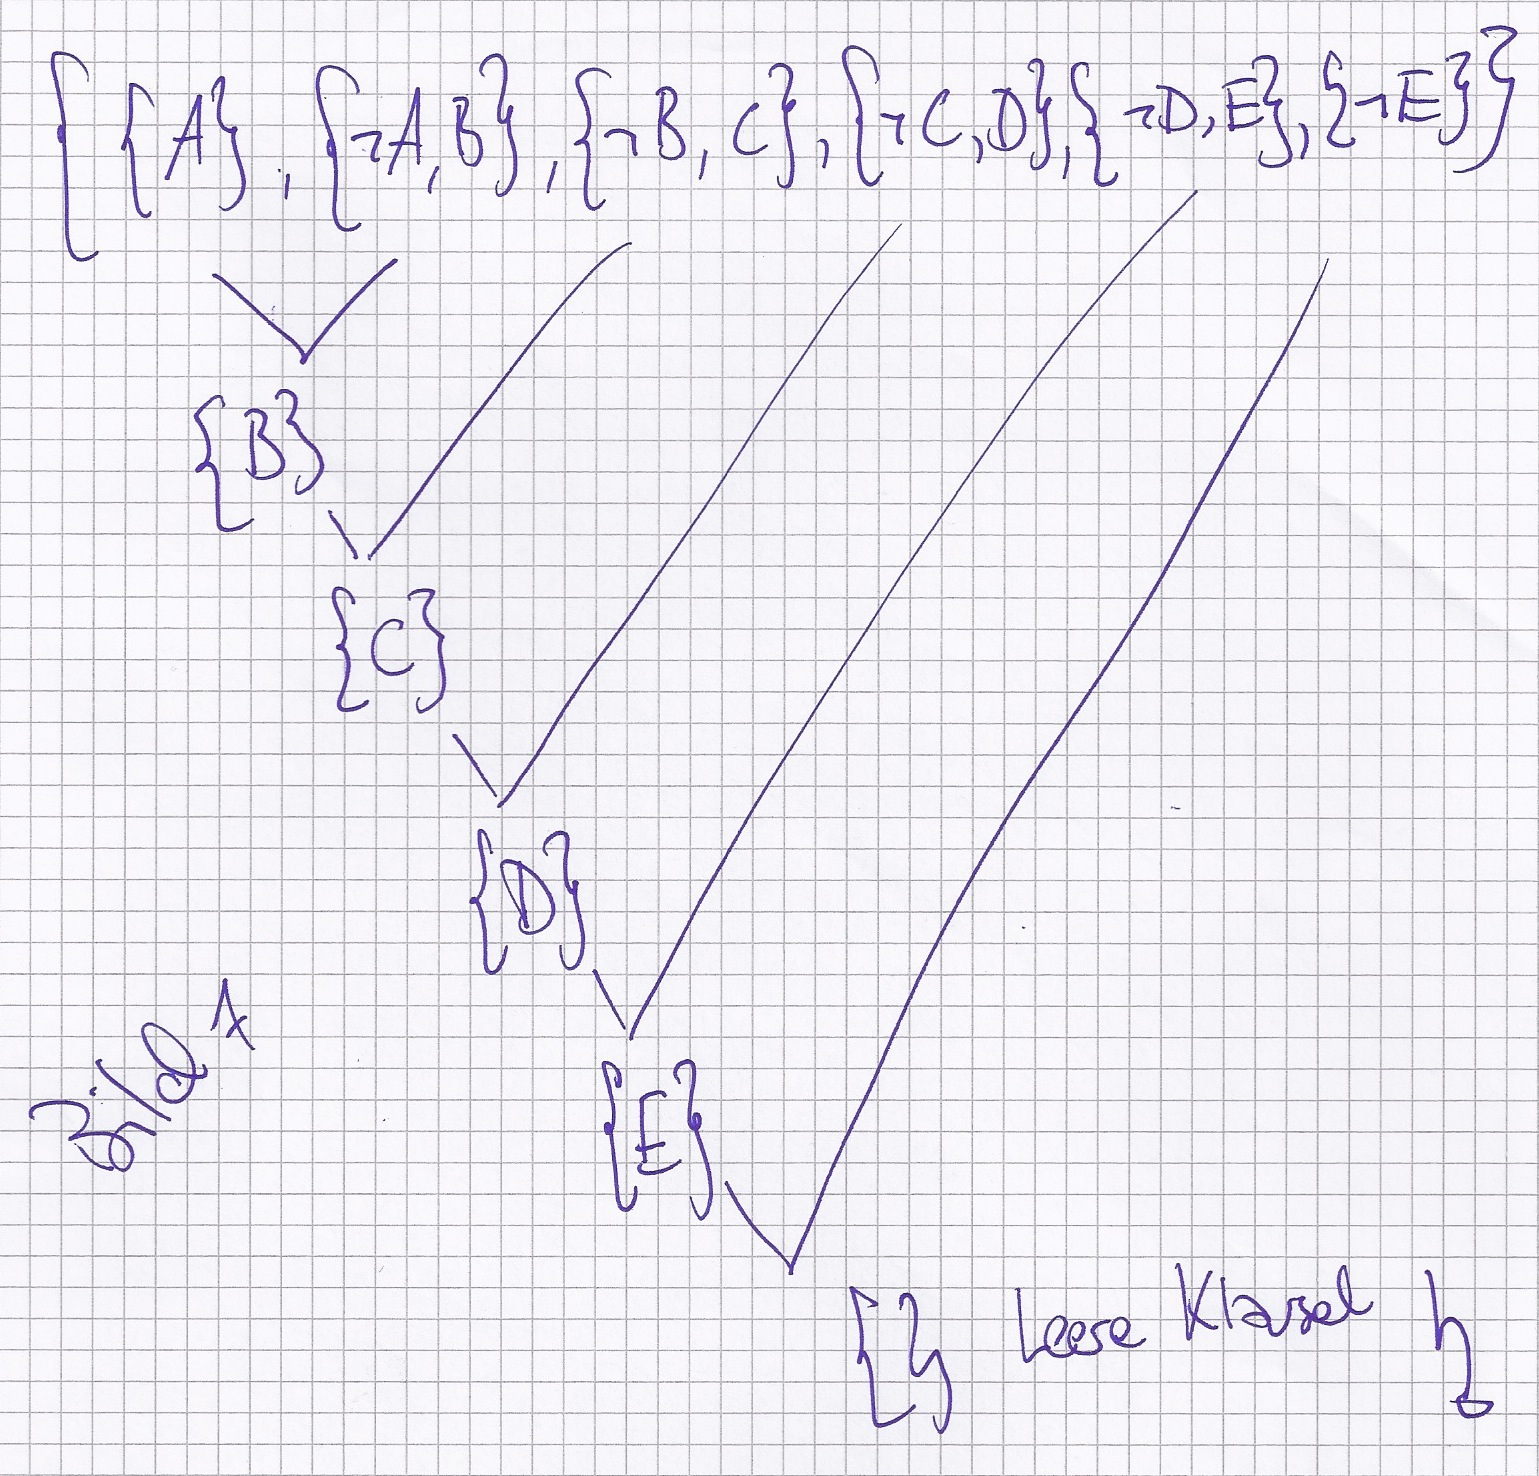
\includegraphics[width=\textwidth]{Bild9}
\end{bsp*}
\begin{bsp*}
	\begin{gather*}
		A \vee B , A \rightarrow C , B \rightarrow C \models C \\
		( A \vee B ) \wedge ( A \rightarrow C ) \wedge ( B \rightarrow C ) \wedge \neg  C \\
		\{ \{ A , B \} , \{ ¬ A , C \} , \{ ¬ B , C \} , \{ ¬ C \} \}
	\end{gather*}
	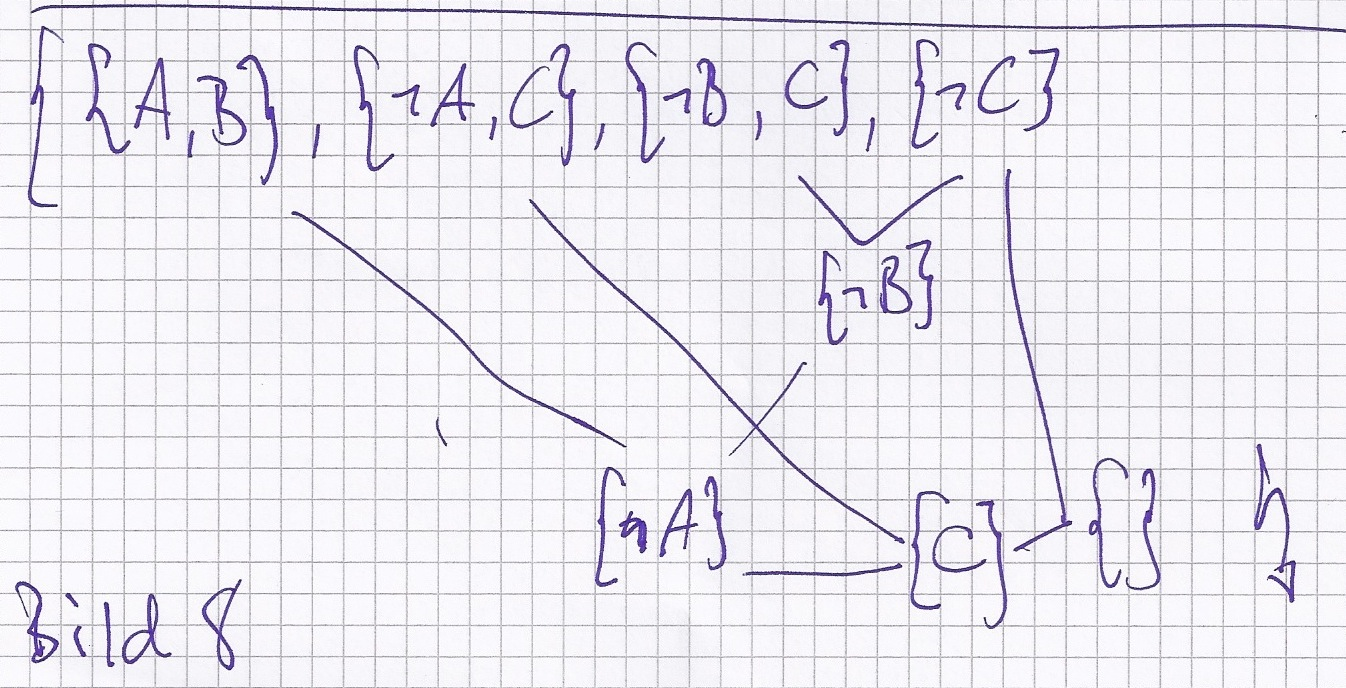
\includegraphics[width=\textwidth]{Bild10}
\end{bsp*}
\begin{bsp*}
	Der entscheidende Schritt: \\
	Jede Belegung die sowohl \\
	$\{ \underset{\uparrow}{A} ,  B , \neg C \}$ als auch $\{ \underset{\uparrow}{\neg A} , \neg E \}$ wahr macht,\\
	muss auch $\{ B , \neg C , \neg E \}$ erfüllen. \\
	Wieso?\\
	\[\begin{array}{ l l l l }
		\text{Fall 1:}	& \mathcal{A}( A ) = 0	& \text{Dann } \{ B , \neg C \} \text{ wahr,}	& \text{also auch } \{ B , \neg C , \neg E \}	\\
		\text{Fall 2:}	& \mathcal{A}( A ) = 0	& \text{Dann } \{ \neg E \} \text{ wahr,}		& \text{also auch } \{ B , \neg C , \neg E \}	
	\end{array}\]
\end{bsp*}
\begin{def*}[note = Resolvent , index = Resolvent]
	$K_1 , K_2 , R$ Klauseln \\
	$\mathbf{R}$ \textbf{Resolvent} von $K_1$ und $K_2$, falls es ein Literal $L$ gibt mit $L \in K_1$ und $\neg L \in K_2 , \mathbf{R=( K_1 \setminus \{ L \} ) \cup ( K_2 \setminus \{ \neg L \} )}$
\end{def*}
\begin{satz*}
	$R$ Resolvent von $K_1 , K_2$. Dann
	\[K_1 , K_2 \models R\]
	Beweis: Übung
\end{satz*}
\begin{bsp*}
	$$F = ( A \vee B \vee \neg C ) \wedge ( \neg A \vee \neg E ) \wedge ( \neg C \vee D \vee E ) \wedge C \wedge ( \neg D \vee \neg C )$$
	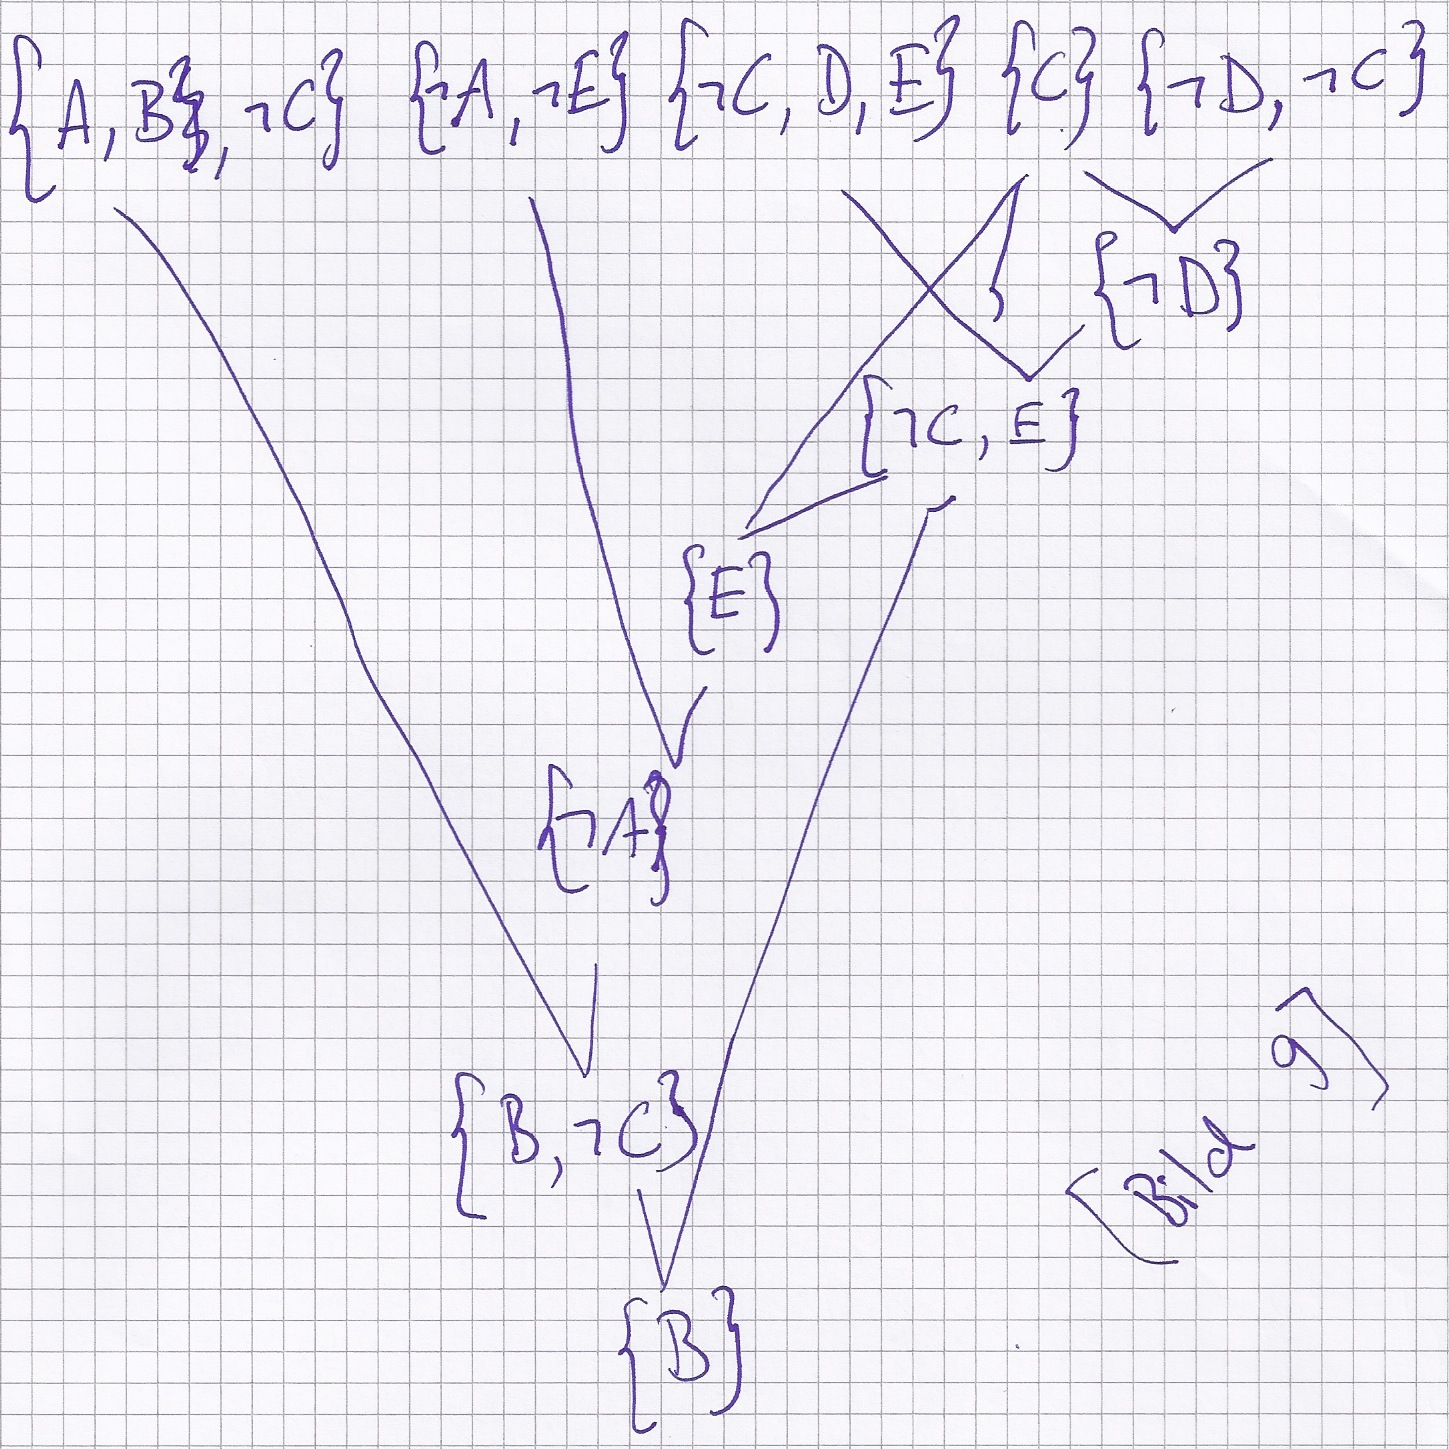
\includegraphics[width=\textwidth]{Bild11}\\
	\begin{itemize}
		\item $\{\}$ lässt sich nicht resolvieren.
		\item F ist erfüllbar und zwar durch $\mathcal{A}( A ) = 0 , \mathcal{A}( B ) = 1 ,$ \\
			$\mathcal{A}( C ) = 1 , \mathcal{A}( D ) = 0 , \mathcal{A}( E ) = 1$
		\item Es gibt keine andere erfüllende Belegung.
	\end{itemize}
\end{bsp*}
\begin{bsp*}
	$F \coloneqq ( \neg B \wedge C \wedge D ) \vee ( \neg B \wedge \neg D ) \vee ( C \wedge D ) \vee B$ \\
	Ist $F$ Tautologie? \\
	Ist $\neg F$ unerfüllbar? \\
	\begin{bew}
		$\neg F \equiv ( B \vee C \vee \neg D ) \wedge ( B \vee D ) \wedge ( \neg C \vee \neg D ) \wedge \neg B$ \\
		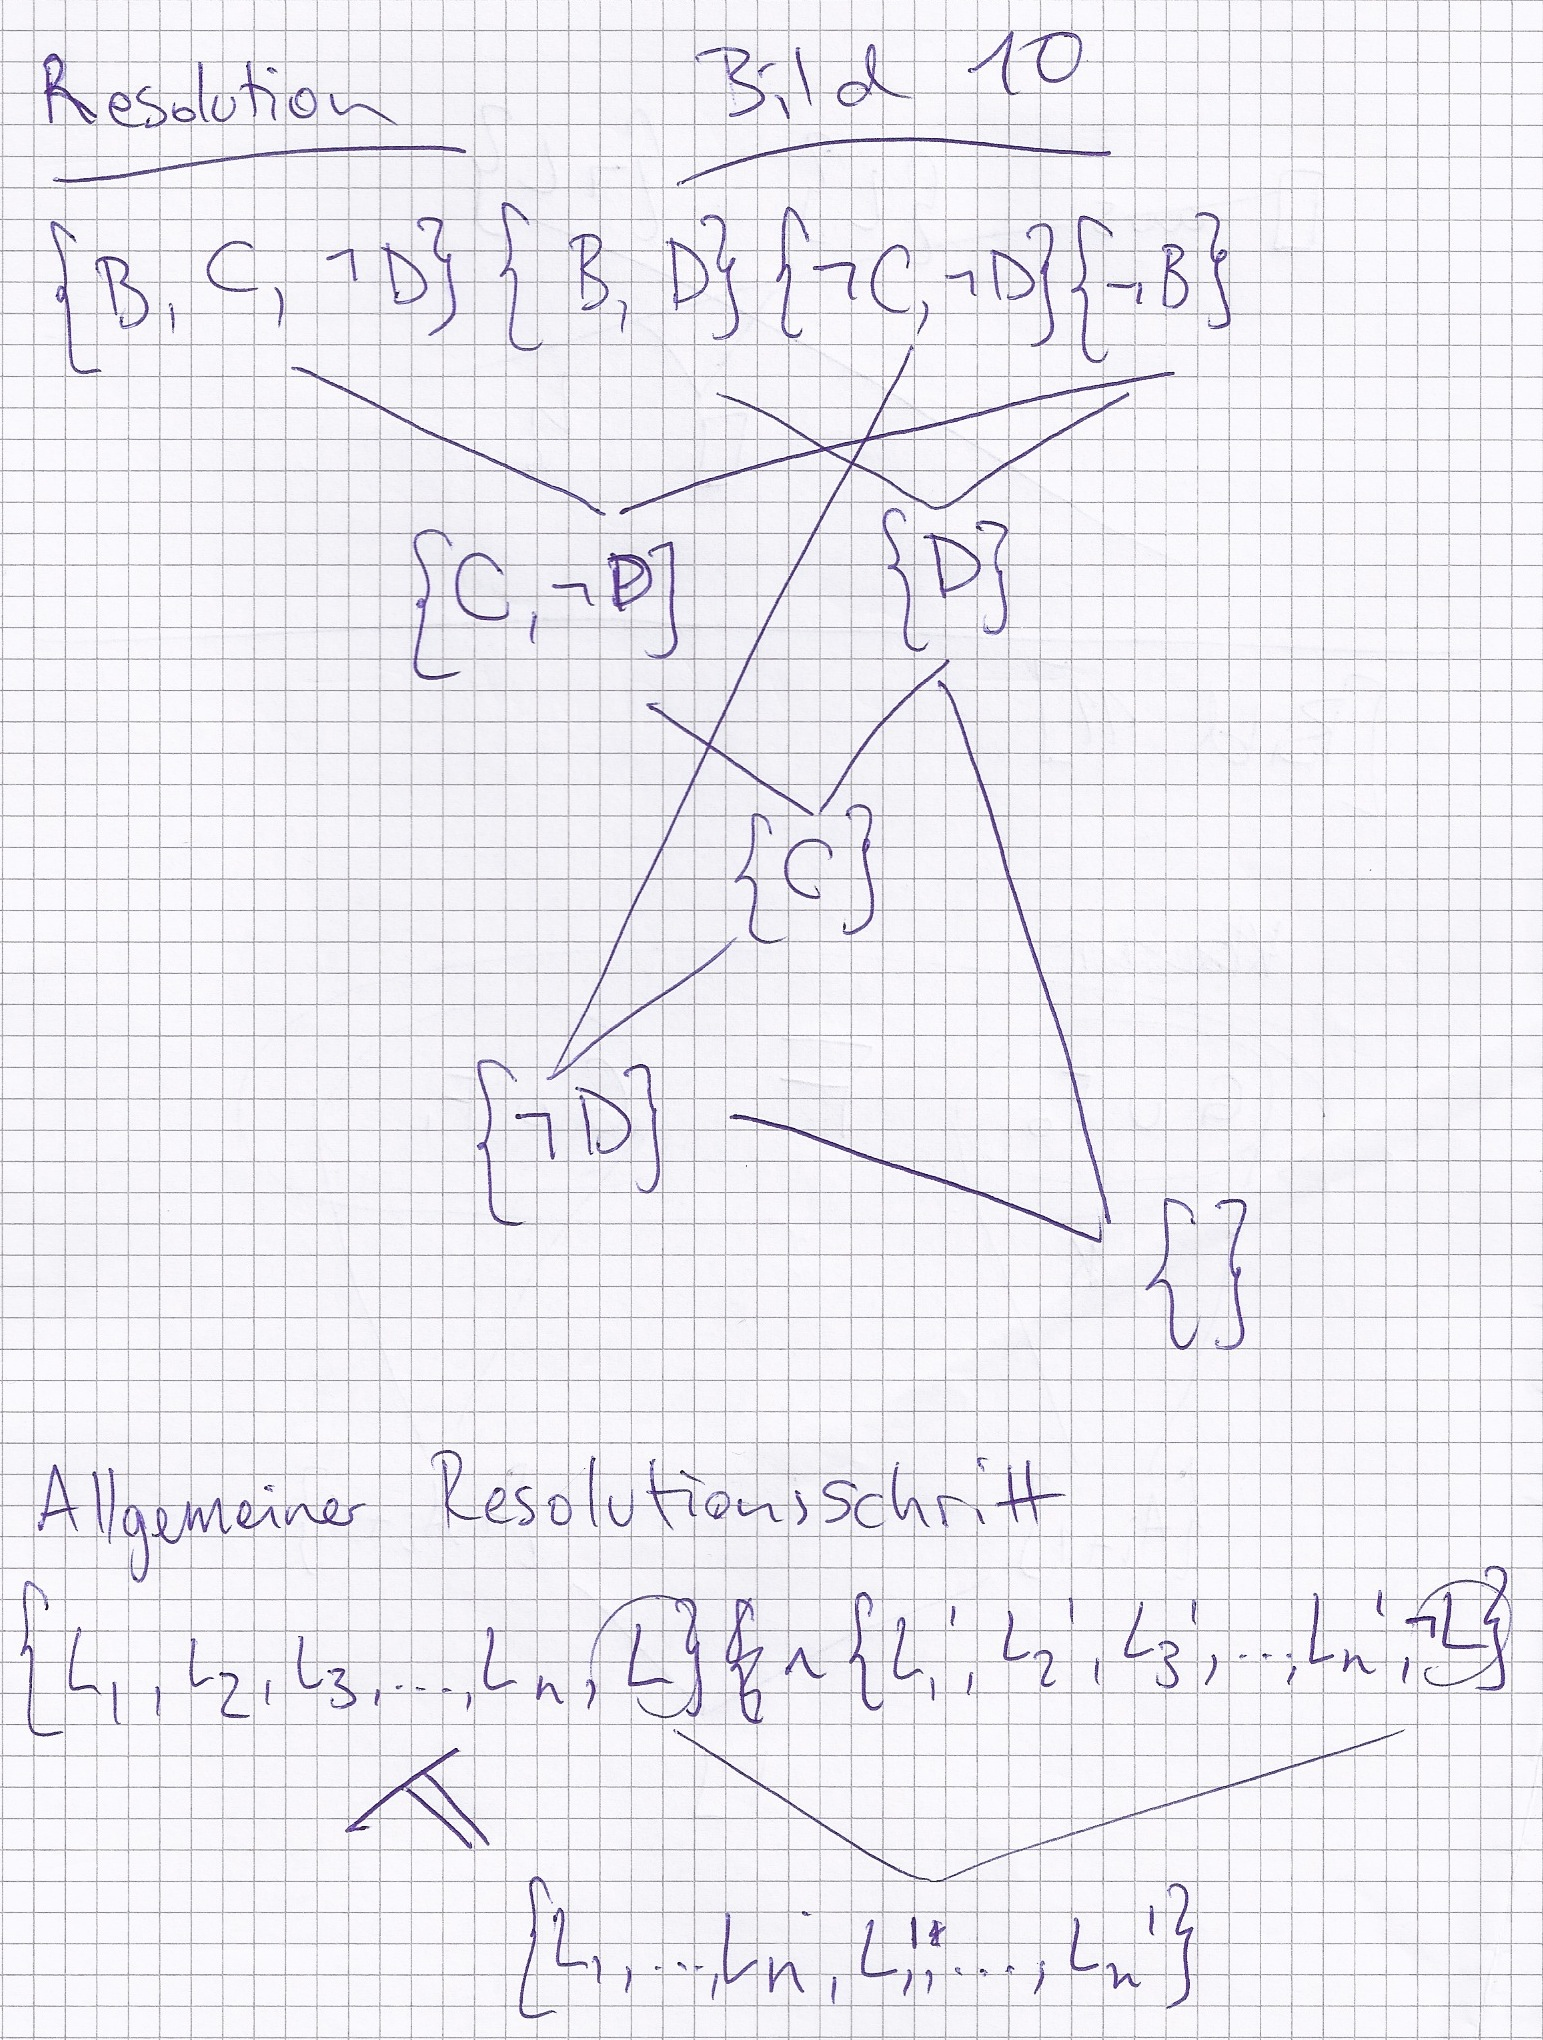
\includegraphics[width=\textwidth]{Bild12}
	\end{bew}
\end{bsp*}

\subsubsection{Was wollen wir von einem Beweiskalkül?}
\begin{description}
	\item[Korrektheit:] ''nichts falsches beweisbar''.
	\begin{itemize}
		\item $F \rightsquigarrow \{\}$, dann $F$ unerfüllbar.
	\end{itemize}
	\item[Vollständigkeit:] ''alles richtige bewiesbar''.
	\begin{itemize}
		\item $F$ unerfüllbar, dann $F \rightsquigarrow \{\}$.
	\end{itemize}
	\item[Effizienz:] Problem: NP-vollständig
	\item[Termination:] bricht ab
\end{description}
$F$ Formel in KNF, Klauselmenge \\
$\Res( F ) \coloneqq \{ \text{Resolvent } R \text{ zweier Klauseln } K_1 , K_2 \text{ in } F \} \cup F$ \\
Dann $\Res( F ) \equiv F$\\
\begin{enumerate}
	\item Prozess $F \rightarrow \Res( F ) \rightarrow \Res( \Res( F ) \rightarrow \dotsb \rightarrow \Resf( F )$ bricht ab.
	\item Falls $F$ unerfüllbar, dann $\Box = \{\} \in \Resf( F )$
\end{enumerate}
\begin{enumerate}
	\item Weil es über einem endlichen Alphabet ( =Atomformeln ) nur endlich viele Klauseln gibt ( als Mengen  ): Nämlich $3^n \text{ über } A_1 , \dotsc , A_n$
	\item Theorem( Hauptsatz der Resolution ) $F$ ist unerfüllbar \gdw $\Box \in \Resf( F )$
	\begin{itemize}
		\item
			\begin{bew}
				$''\Leftarrow'' \Box \text{ aus } \{ L \} \{ \neg L \} \: \text{\lightning}$
			\end{bew}
		\item
			\begin{bew}
				$''\Rightarrow'' \text{ Induktion über Anzahl } n \text{ Atomformeln}$
				\begin{itemize}
					\item Verankerung $n=1$ \\
					\begin{gather*}
						\begin{array}{ l l }
							F \equiv \{ \{ A_1 \} \}									\\
							F \equiv \{ \{ \neg A_1 \} \}								\\
							F \equiv \{ \{ \} \}  = \{ \Box \}							\\
							F \equiv \{ \{ A_1 \} \{ \neg A_1 \} \}	& (A_1 \wedge \neg A_1 )	\\
							F \equiv \{ \{ A_1 , \neg A_1 \} \}		& ( A_1 \vee \neg A_1 )	
						\end{array}
					\end{gather*}
					\item Induktionvoraussetzung:
					\begin{itemize}
						\item Richig für $A_1 , \dotsc , A_i$
					\end{itemize}
					\item Induktionsschritt:
					\begin{itemize}
						\item Richtig für $A_1 , \dotsc , A_{i+1}$
						\item $G$ Klauseln ohne $A_{i+1} , \neg A_{i+1}$
						\item
							\begin{gather*}
								F_0 \text{ Klauseln mit } A_{i+1} \\
								F_1 \text{ Klauseln mit } \neg A_{i+1} \\
								F_0' \coloneqq \{ K \setminus \{ A_{i+1} \} \mid K \in F_0 \} \\
								F_1' \coloneqq \{ K \setminus \{ A_{i+1} \} \mid K \in F_1 \}
							\end{gather*}
						\item
							\begin{description}
								\item[Fall 1:] $G \text{ unerfüllbar } \implies \Box \in \Resf( G ) \implies \Box \in \Resf( F )$
								\item[Fall 2:] $G \text{ erfüllbar. Es gilt } G \cup F_0' \text{ unerfüllbar}$
								\begin{itemize}
									\item Indirekt. $G \cup F_0'$ erfüllbar.
									\begin{gather*}
										\text{Belegung } \mathcal{A}\{ A_1 , \dotsc , A_i \} \rightarrow \{ 0 , 1 \} \\
										\text{Zusätzlich } \mathcal{A}( A_{i+1} ) = 0 \\
										\mathcal{A} \text{ erfüllt: } G , F_0 , F_1 , \text{ also F \lightning  Theorem }
									\end{gather*}
									\item Analog $G \cup F_1'$ unerfüllbar
								\end{itemize}
							\end{description}
					\end{itemize}
					\item Induktionsvoraussetzung: \\
						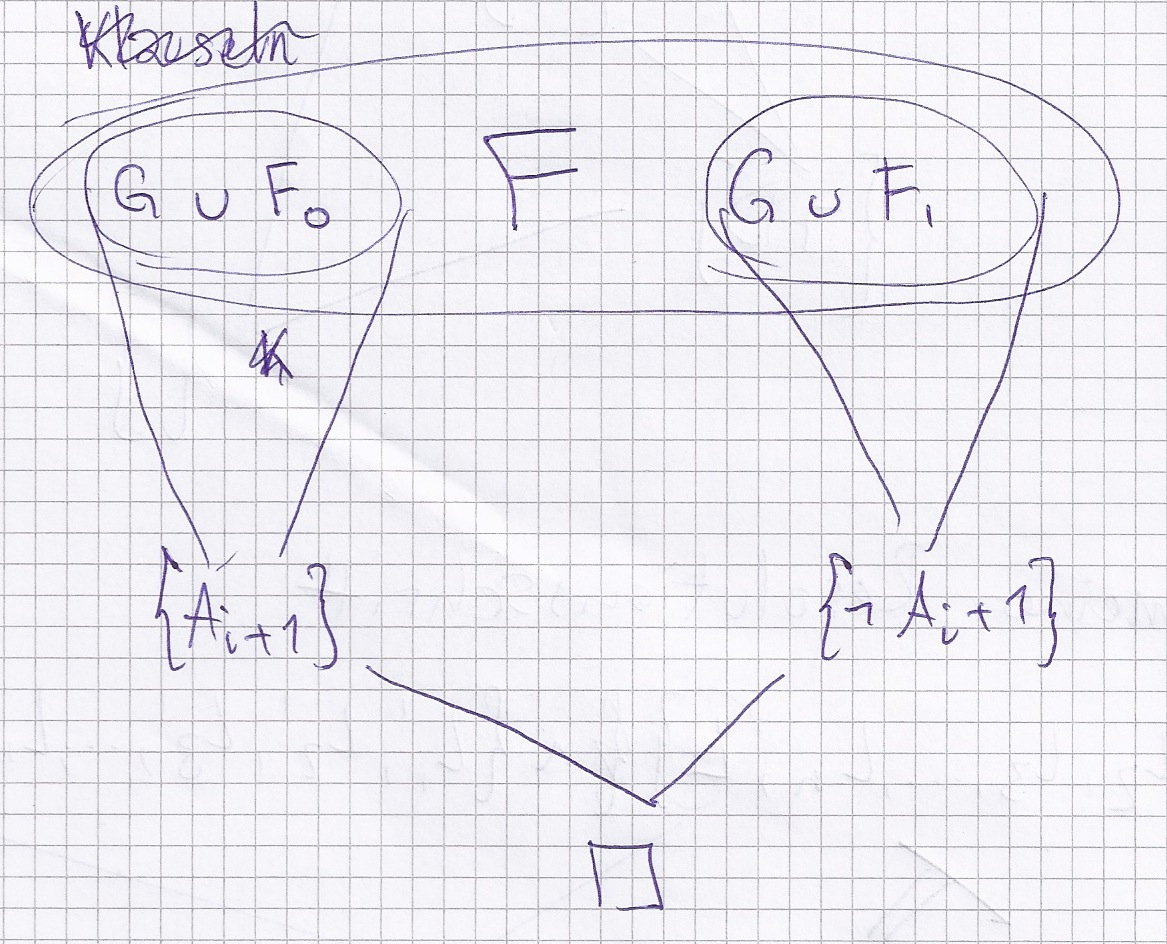
\includegraphics[width=\textwidth]{Bild13}
				\end{itemize}
			\end{bew}
	\end{itemize}
\end{enumerate}
\todo{Vertical spacing}
\todo{Too long}

\subsubsection{Resolutionsalgorithmus}
\begin{algorithmic}
\REQUIRE $F$ in KNF
\REPEAT
	\STATE $G \coloneqq F$
	\STATE $F \coloneqq \Res( F )$
\UNTIL{ $\Box \in F$ or $F = G$}
\IF{ $\Box \in F$ }
	\PRINT ''unerfüllbar''
\ELSE
	\PRINT ''erfüllbar''
\ENDIF
\end{algorithmic}

\subsubsection{Effizienter Spezialfall: Hornlogik}
Hornformel: $A_1 \wedge A_2 \wedge \dotsb \wedge A_n \rightarrow B \equiv \{ \neg A_1 , \neg A_2 , \dotsc , \neg A_n , B \}$ \\
\begin{def*}[note = Hornformel , index = Hornformel]
	\textbf{Eine Hornformel hat höchstens ein positives (nicht-negatives) Literal.}
\end{def*}
\begin{bsp*}
	\begin{gather*}
		\left.\begin{array}{ l }
			\left.\begin{array}{ l l }
				A							& \{ A \}					\\
				B							& \{ B \}					\\
				C							& \{ C \}					
			\end{array} \right\} \textbf{Fakten}	\\
			\left.\begin{array}{ l l }
				A \wedge B \wedge E \rightarrow F	& \{ \neg A , \neg B , \neg E , F \}	\\
				C \wedge D  \rightarrow G			& \{ \neg C , \neg D , G \}		\\
				B \wedge C  \rightarrow D			& \{ \neg B , \neg C , G \}		\\
				G \wedge A  \rightarrow E			& \{ \neg G , \neg A , E \}		
			\end{array} \right\} \textbf{Regeln}
		\end{array} \right\} \textbf{Datenbank}	\\
		\text{Gilt } E \text{? (\gdw Datenbank } \cup \{ \neg E \} \text{ unerfüllbar ) } \textbf{Abfrage}
	\end{gather*}
\end{bsp*}
2 Approaches:
\begin{itemize}
	\item Markierungsalgorithumus (Bottom-up)
	\item Lineare Resolution (Top-down)
\end{itemize}

\section{Elemente Der Prädikatenlogik}
Die Aussagenlogik ist eine heile Welt. Aber sie ist zu schwach für die Formulierung und Formalisierung der meisten Mathematischen Tatsachen.\\
\begin{bsp}
	Alle Menschen sind sterblich. \\
	Sokrates ist ein Mensch. \\
	$\drsh$ ? \\
	\begin{itemize}
		\item $\forall x ~ ( \text{Mensch}( x ) \rightarrow \text{Sterblich}( x )$
		\begin{itemize}
			\item Quantisierung über ein Universum.
			\item Prädikate, Eigenschaft $\rightarrow \{ 0 , 1 \}$
			\item Aussagenlogik ( AL ) ist Teil der Prädikatenlogik ( PL ) .
		\end{itemize}
		\item Mensch$($ SOKRATES $)$
			\begin{itemize}
				\item Konstanten
			\end{itemize}
	\end{itemize}
	Mensch$($ SOKRATES $) \rightarrow$ Sterblich$($ SOKRATES $)$
\end{bsp}
\begin{bsp}
	Was ''sagen'' folgende Formeln?\\
	\begin{itemize}
		\item $\forall x \forall \epsilon \exists \delta \forall y~( d( x, y )  < \delta \rightarrow d( f( x ) , f( y ) ) < \epsilon )$
		\begin{itemize}
			\item Quantoren: Universum z.B. $\mathbb{R}^{>0}$
			\item Interpretation von: \\
			\begin{tabular}{ l l }
				''$<$''		& : $<$			\\
				''$d( x , y )$''	& : $\abs{x-y}$		\\
				''$f( x )$''		& : $f( x ) = x^2$	
			\end{tabular}
		\end{itemize}
		\item $\forall n \exists p \forall a \forall b~(p > n \wedge ( p = a \cdot b \rightarrow a = 1 \oplus b = 1 ) )$
		\begin{itemize}
			\item ''Es gibt unendlich viele Primzahlen.''
			\item Struktur: \\
			\begin{tabular}{ l l }
				Universum	& : $\mathbb{N}$		\\
				''$>$''	& : $>$				\\
				''$\cdot$''	& : $\cdot$			\\
				''$1$''	& : $1 \in \mathbb{N}$	
			\end{tabular}
		\end{itemize}
		\item $\exists n \exists a \exists b \exists c~( n \geq 3 \wedge a^n + b^n = c^n )$
		\begin{itemize}
			\item Struktur:
			\begin{itemize}
				\item Universum: $\mathbb{N}$
				\item $\geq , 3 , ^ , +$ wie üblich
			\end{itemize}
			\item \textbf{grosser fermatscher Satz\index{grosser fermatscher Satz}}
			\item falsch
			\item In der PL ist schon das Auswertensproblem schwierig.
		\end{itemize}
	\end{itemize}
\end{bsp}
\begin{bsp*}
	\begin{gather*}
		\forall x~( x \geq 4 \wedge \exists y~( x = 2 \cdot y ) \\
		\quad \rightarrow \exists p \exists q~( x = p + q \wedge \Prim( p ) \wedge \Prim( q ) ) ) \\
		\Prim( r ) \coloneqq ( r = a \cdot b \rightarrow a = 1 \oplus b = 1 )
	\end{gather*}
	\begin{itemize}
		\item Struktur:
		\begin{itemize}
			\item Universum: $\mathbb{N}$
			\item ''übliche'' Interpretationen:
			\begin{itemize}
				\item Konstanten: $1 , 2 , 4$
				\item Funktionen: $+ , \cdot$
				\item Prädikate: $\geq , ( = )$
			\end{itemize}
		\end{itemize}
		\item Allen geraden Zahlen $\geq 4$ können als Summe zweier Primzahlen geschrieben werden. ( \textbf{Goldbach-Vermutung\index{Goldbach-Vermutung}} )
		\item Niemand weiss, ob diese Struktur ein Modell ist für die Formel.
	\end{itemize}
\end{bsp*}
\begin{bem}
	\begin{tabular}{ l l }
		Struktur $\models$ Formel		& ( ist ein Modell )		\\
		$F \models G$				& (semantische Folgerung)	\\
		$F \equiv G$				& (semantische Äquivalnez)	\\
		Tautologie (=gültige Formel):	& jede Struktur ist Modell	\\
		Unerfüllbare Formel:			& keine Struktur ist Modell	
	\end{tabular}
\end{bem}
\begin{bsp*}{Äquivalenzen und gültigen Formeln}
	\begin{itemize}
		\item $\forall x~( P( x ) ) \rightarrow P( c ) \qquad \forall x~( P( x ) ) \models P( c )$
		\item $P( c ) \rightarrow \exists x~( P( x ) ) \qquad ( c ) \models \exists x~( P( x ) )$
		\item $\neg \forall x~( P( x ) ) \equiv \exists x~( P( x ) )$
		\item $\neg \exists x~( P( x ) ) \equiv \forall x~( P( x ) )$
		\item $\forall x~( P( x ) \wedge Q( x ) ) \equiv \forall x~( P( x ) ) \wedge \forall x~( Q( x ) ) \equiv \forall x~( P( x ) ) \wedge \forall y~( Q( y ) )$
		\item $\exists x~( P( x ) \vee Q( x ) ) \equiv \exists x~( P( x ) ) \vee \exists x~( Q( x ) ) \equiv \exists x~( P( x ) ) \vee \exists y~( Q( y ) )$
		\item $\forall x~( P( x ) \vee Q( x ) ) \Leftarrow \forall x~( P( x ) ) \vee \forall y~( Q( y ) )$  \quad \textbf{ABER NICHT UMGEKEHRT} (mögliche Interpretation: ''Alle Zahlen sind gerade oder ungerade.'' )
		\item $\exists x~( P( x ) \wedge Q( x ) ) \Rightarrow \exists x~( P( x ) ) \wedge \exists y~( Q( y ) )$  \quad \textbf{ABER NICHT UMGEKEHRT} (mögliche Interpretation: ''retation: Es gibt gerade und es gibt ungerade Zahlen.'' )
		\item $\forall x \forall y P( x , y ) \equiv \forall y \forall x P( x , y )$
		\item $\exists x \exists y P( x , y ) \equiv \exists y \exists x P( x , y )$
		\item $\forall x \exists y P( x , y ) \Leftarrow \exists y \forall x P( x , y )$ \quad \textbf{ABER NICHT UMGEKEHRT}
	\end{itemize}
\end{bsp*}

\subsection{Ist das Erfüllbarkeitsprobelm der PL algorithmisch entscheidbar?}
\begin{itemize}
	\item AL \\
		\[
			F \text{ erfüllbar } \rightarrow \begin{array}{l}
				\text{Algorithumus}		\\
				\text{Wahrheitstabelle}	\\
				\text{Resolution}			
			\end{array} \begin{array}{l}
				\rightarrow \text{ ''ja''}		\\
				\rightarrow \text{ ''nein''}	
			\end{array} \qquad \qquad \textbf{entscheidbar}
		\]
	\item PL \\
	\begin{gather*}
		F \text{ erfüllbar } \rightarrow \text{ jede mögliche Struktur einsetzen} \begin{array}{l}
			\rightarrow \text{\Interval} \\
			\rightarrow \text{\Interval}
		\end{array} \\
		F \text{ erfüllbar } \rightarrow \text{ ''Resolution'', Unifikation} \begin{array}{l}
			\rightarrow \text{\Interval} \\
			\rightarrow \text{''nein''}
		\end{array} \textbf{semi-entscheidbar}
	\end{gather*}
\end{itemize}
Ist die PL entscheidbar? \\
\textbf{NEIN}\\
Sie wäre es, wenn es möglich wäre, zu ntscheiden, ob ein gegebener Algorithmus auf einem gegebenen Input abhält.\\
Halteproblem:
\begin{itemize}
	\item Annahme: Es geht.
	\item 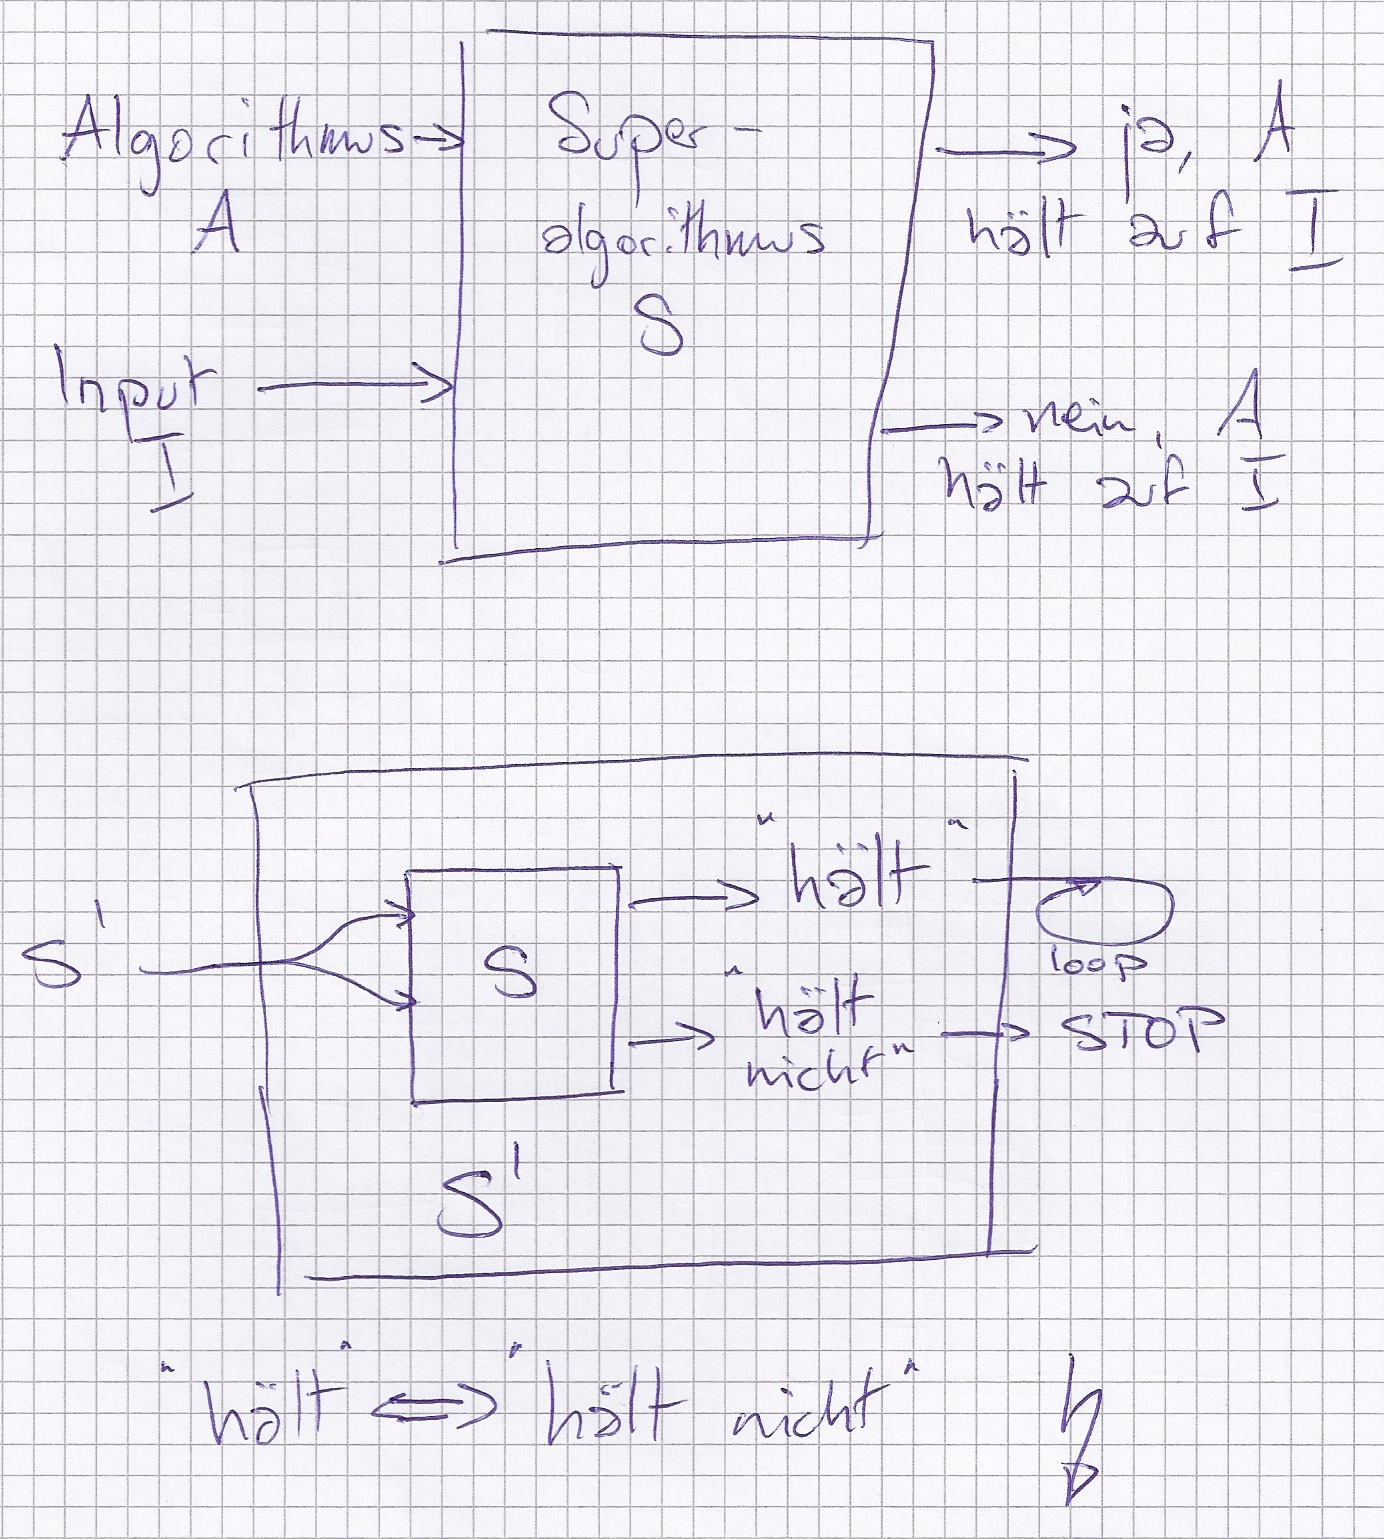
\includegraphics[width=\textwidth]{Bild14}
	\item Das Halteproblem ist nicht entscheidbar $\implies$ die PL ist nicht entscheidbar.
\end{itemize}

\subsection{Selbstbezüglichkeit als Quelle von Paradoxa, Einsichten, Katostrophen}
\begin{itemize}
	\item (Hofstadter)
	\item Epinemides (aus Kreta): ''Alle Kreter sind Lügner.''
	\begin{itemize}
		\item ''Ich bin falsch.''
	\end{itemize}
	\item Wie viele Buchstaben hat die Antwort auf diese Frage?
	\begin{itemize}
		\item Vier
	\end{itemize}
	\item ''Die kleinste Zahl, die sich nicht durch einen deutschen Satz mit höchstens zwanzig Wörtern beschreiben lässt.''
	\begin{itemize}
		\item 16
	\end{itemize}
	\item Gödel:
	\begin{itemize}
		\item Hilberts Traum: Formales System, in dem alles richtige beweisbar ist. $\eqqcolon \Delta$
		\item Formeln $F$ und Beweise $B$ sind Strings / natürliche Zahlen.
		\item Prädikat $Abl( B, F )$ \qquad ''B beweist F.''
		\item $F_i( x ) , i = 1 , 2 , \dotsc$ \qquad Alle Formeln mit Variable $x$.
		\item $\neg \exists B~( Abl( B , F_x( x ) ) = F_{i_0}( x )$
		\item $\neg \exists B~( Abl( B , F_{i_0}( i_0 ) ) = F_{i_0}( i_0 )$
	\end{itemize}
\end{itemize}

\chapter{Mengenlehre}
\section{Grundbegriffe}
Elementbeziehung:\\
\begin{gather*}
	x \in A : \text{Objekt } x \text{ ist Element der Menge } A \\
	x \notin A : \iff \neg ( x \in A )
\end{gather*}

\subsection{Cantor: ''naiv'': Jedes Objekt (insbes. jede Menge ) kann in jeder Menge sein oder nicht.}
Eine Menge kann sich selbst enthalten.\\
Problem: \textbf{Russel Antinomie}\index{Russel Antinomie}:\\
''Ein Barbier rasiert jeden, der sich selbst nicht rasiert. Rasiert er sich selbst?'' \\
\begin{gather*}
	\begin{array}{ l l }
		M \coloneqq \{ A \mid A \notin A \}			& M \in M ?				\\
		M \in M \implies M \notin M \implies M \in M	&\text{Nicht entscheidbar.}	
	\end{array}
\end{gather*}\\
\begin{tabular}{ l p{7cm} }
Ausweg: \textbf{Klassen}\index{Klasse} (Eigenschaften),	&\textbf{Mengen}\index{Menge} \\
										& $\drsh$ Axiomensystem ZFC (Zermelo Fränkel ''Choice'' (Auswahlaxiom))
\end{tabular}

\subsubsection{Auswahlaxiom}
Konsequenz: \text{Banach-Tarski-Paradox}\index{Banach-Tarski-Paradox}: \\
Eine Kugel in 5 teilen und daraus 2 gleich grosse Kugeln bilden.

\subsection{Wie darf man Mengen bilden?}
Mengen dürfen weiter Mengen enthalten, eg. $\{ \N , \R \}$

\subsubsection{Gleichheit von Mengen (Extensionalitätsaxiom)}
\begin{gather*}
	A , B \text{ Mengen} \\
	\begin{aligned}
		\text{Dann } A = B	&\iff \forall x~( x \in A \leftrightarrow x \in B ) \\
						&''\Rightarrow'': \text{ Logik der Gleichheit} \\
						&''\Leftarrow'': \text{ Axiom}
	\end{aligned}
\end{gather*}\\
\begin{bsp*}
	\[ \{ a , b , c \} = \{ b , c , a \} = \{ a , a , b , c \} \neq \{ \{ a \} , \{ b \} , \{ c \} \} \]
\end{bsp*}

\subsubsection{Mengenbildung mit Prädikaten}
\begin{gather*}
	A \text{ Menge}, P( \cdot ) \text{Prädikat} \\
	\text{Dann ist } B = \{ x \in A \mid P( x ) \}
\end{gather*} \\
\begin{bsp*}
	\begin{gather*}
		A = \{ x \in \mathbb{N} \mid 0 \leq x \leq 10 \} = \{ 0 , 1 , 2 , 3 , 4 , 5 , 6 , 7 , 8 , 9 , 10 \} \\
		B = \{ x \in A \mid \Prim( x ) \} = \{ 2 , 3 , 5 , 7 \}
	\end{gather*}
\end{bsp*}

\subsubsection{Teilmengenrelation}
\[ A \subseteq B : \iff \forall x~( x \in A \rightarrow x \in B ) \]
\begin{satz*}
	$A \subseteq B \wedge B \subseteq A \implies A = B$ \\
	Beweis: Extensionalität
\end{satz*}

\subsubsection{Existenz}
Es gibt mindestens eine Menge.
\begin{gather*}
	A \text{ Menge.} \\
	\varnothing \coloneqq \{ x \in A \mid x \neq x \} \\
	\text{Dann gilt für jede Menge } B: \\
	\varnothing \subseteq B .
\end{gather*}
\begin{gather*}
	\text{Die ganze Mathematik wird aus } \varnothing \text{ konstruiert.} \\
	\begin{aligned}
		\varnothing											& \eqqcolon 0	\\
		\{ \varnothing \}											& \eqqcolon 1	\\
		\{ \varnothing , \{ \varnothing \} \}							& \eqqcolon 2	\\
		\{ \varnothing , \{ \varnothing \} , \{ \varnothing , \{ \varnothing \} \} \}	& \eqqcolon 3	\\
		\mathbb{N} \coloneqq \{ 0 , 1 , 2 , 3 , \dotsc \}					& = \omega	\\
		\{ 0 , 1 , 2 , 3 , \dotsc , \omega \}								& = \omega + 1
	\end{aligned}
\end{gather*}

\subsubsection{Mengenbildungen}
Falls $A$ und $B$ Mengen sind, dann auch:
\begin{align*}
	& A \cap B : x \in A \cap B :\iff x \in A \wedge x\in B					& \text{Durchschnitt}			\\
	& A \cup B : x \in A \cup B :\iff x \in A \vee x\in B						& \text{Vereinigung}			\\
	& A \setminus B : x \in A \setminus B :\iff x \in A \wedge x\notin B			& \text{Durchschnitt}			\\
	& A \bigtriangleup B : x \in A \bigtriangleup B :\iff x \in A \oplus x\in B		& \text{symmetrische Differenz}	\\
	& \mathbb{P}( A ) = 2^A : x \in \mathbb{P}( A ) :\iff x \subseteq A			& \text{Potenzmenge}			\\
	\multicolumn{2}{l}{\text{Falls Universum } U \text{ Menge:}}										\\
	&\overline{A} \coloneqq U \setminus A								& \text{Komplementärmenge}	
\end{align*}
\[ \overline{A \setminus B} \]

\subsubsection{Mengenfamilien}
\begin{gather*}
	A_i \text{ Menge für } i \in I , I \text{ Menge} \\
	\begin{aligned}
	& x \in \bigcup_{i \in I} A_i :\iff \exists i \in I : x \in A_i 		& \bigcup_{i \in \varnothing} A_i = \varnothing \\
	& x \in \bigcap_{i \in I} A_i :\iff \forall i \in I : x \in A_i 		& \bigcup_{i \in \varnothing} A_i \text{ darf nicht existieren } \rightarrow \text{Russel Antinomie}
	\end{aligned}
\end{gather*}

\subsubsection{Das kartesische Produkt (Descartes, 17 Jh.)}
Das geordnete Paar
\begin{gather*}
	(a , b) = (c , d) :\iff a = c \wedge b = d \\
	\intertext{Definition als Menge:}
	(a , b) \coloneqq \{ \{ a \} , \{ a , b \} \} \qquad (a , a) = \{ \{ a \} , \{ a , a \} \} = \{ \{ a \} , \{ a \} \} = \{ \{ a \} \}\\
	\\
	A , B \text{ Mengen.} \\
	A \times B \coloneqq \{ (a , b) \mid a \in A \wedge b \in B \} \\
	A \times B \neq B \times A \text{ falls } A \neq B \\
	I = \{ 1 , 2 , \dotsc , k \} \\
	\bigtimes_{i=0}^k A_i \coloneqq \{ (a_1 , \dotsc , a_k ) \mid \forall i : a_i \in A_i \}
\end{gather*}
\begin{bsp*}
	\begin{gather*}
		\mathbb{R} \times \mathbb{R} \\
		R \subseteq \mathbb{R} \times \mathbb{R} \\
		R = \{ (x , y) \in \mathbb{R}^2 \mid x \leq y \}
	\end{gather*}
\end{bsp*}

\section{Relationen}
\begin{def*}[note = Relation , index = Relation]
	Eine (binäre) Relation $\mathrm{R}$ von $A$ nach $B$ ist $\mathrm{R} \subseteq A \times B$ . \\
	Relation auf $A$: $\mathrm{R} \subseteq A \times A = A^2$
\end{def*}
\[
	\text{Wir schreiben } \begin{array}{ l l l }
		a &\mathrm{R}		&b			\\
		a &\leq			&b			\\
		a &\not{\mathrm{R}}	&b			\\
		a &\not\leq		&b	
	\end{array} \text{ für } \begin{array}{ l l l }
		(a , b) &\in			&\mathrm{R}	\\
		(a , b) &\in			&\leq			\\
		(a , b) &\notin		&\mathrm{R}	\\
		(a , b) &\notin		&\leq		
	\end{array}
\]
Jetzt sind die Relationen Mengen $\rightarrow$ Mengenkalkül
\begin{gather*}
	\leq~\cap~\geq~=~= \\
	\leq~\bigtriangleup~\geq~=~\neq \\
	<~\subseteq~\leq~=~\overline{\geq}~=~\leq
\end{gather*}
\begin{bsp*}{Relationen auf $\Z$}
	$\mathrm{R} \subset \mathbb{Z} \times \mathbb{Z}$ \\
	\begin{itemize}
		\item $\mid$ Teilbarkeit: \quad $(a , b) \in \mid :\iff \exists c \in \mathbb{Z} : a \cdot c = b$
		\item $\leq$
		\item $\equiv \pmod m \quad a \equiv b \pmod m :\iff m \mid (a - b)$ \\
			$ \equiv_m \cap \equiv_n = \equiv_{kgV(m,n)}$
	\end{itemize}
\end{bsp*}

\subsubsection{Darstellung von Relationen}
falls $|A| , |B| < \infty$\\
Relation $\mathrm{R}$ von $A$ nach $B , \mathrm{R} \subseteq A \times B$\\
\begin{description}
	\item[Als (binäre) Matrix] Eintrag ist $1$ falls $(a , b) \in \mathrm{R}$, sonst $0$
	\item[Als bipartiter Graph] 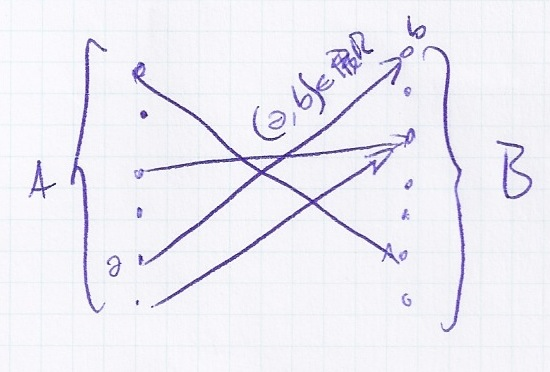
\includegraphics{Bild15}
	\item[Falls $A = B$] 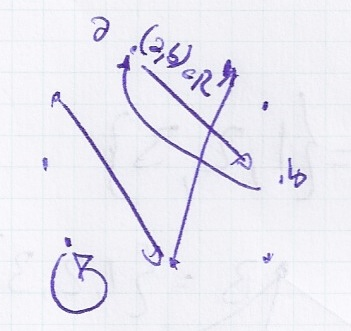
\includegraphics{Bild16}
\end{description}

\subsubsection{Eigenschaften von Relationen (auf \texorpdfstring{$A$}{A})}
\begin{description}
	\item[reflexiv:] $\forall a \in A : (a , a) \in \mathrm{R}$
		\begin{itemize}
			\item Matrix: Diagonale lauter 1 \\
				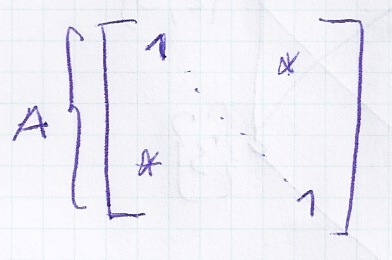
\includegraphics{Bild17}
			\item Graph: jede Punkt mit sich selbst (loop) \\
				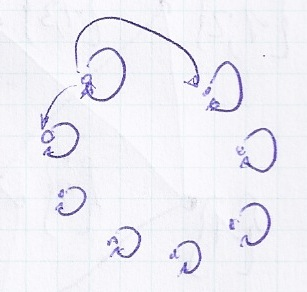
\includegraphics{Bild18} \\
			\begin{bsp*}{reflexive Relationen}\\
				\begin{itemize}
					\item $\leq$
					\item $=$
					\item $|$
					\item $\subseteq$
					\item $\equiv_m$
				\end{itemize}
			\end{bsp*}
			\begin{bsp*}{nicht reflexive Relationen}
				\begin{itemize}
					\item $<$
					\item $>$
					\item $\subset$
					\item $\nmid$
					\item $\neq$
					\item $\in$
				\end{itemize}
			\end{bsp*}
		\end{itemize}
	\item[antireflexiv:] $\forall a \in A : (a , a) \notin \mathrm{R}$
		\begin{itemize}
			\item Matrix: Diagonale lauter $0$
			\item Graph: Kein Punkt mit sich selbst
		\end{itemize}
	\item[symmetrisch:] $\forall a , b \in A : (a , b) \in \mathrm{R} \iff (b , a) \in \mathrm{R}$
		\begin{itemize}
			\item Matrix: symmetrisch $(M^T = M)$
			\item Graph: alle Pfeile beidseitig (werden als Linien ohne Pfeilköpfe dargestellt) \\
			\begin{bsp*}{symmetrische Relationen}
				\begin{itemize}
					\item $=$
					\item $\equiv_m$
				\end{itemize}
			\end{bsp*}
		\end{itemize}
	\item[antisymmetrisch:] $\forall a , b \in A : (a , b) \in \mathrm{R} \wedge (b , a) \in \mathrm{R} \implies a = b$\\
		\begin{bsp*}{antisymmetrische Relationen}
			\begin{itemize}
				\item $\leq$
				\item $|$ auf $\mathbb{N}$
				\item $<$
				\item $=$
			\end{itemize}
		\end{bsp*}
	\item[transitiv:] $\forall a , b , c \in A : (a , b) \in \mathrm{R} \wedge (b , c) \in \mathrm{R} \implies (a , b) \in \mathrm{R}$\\
		\begin{itemize}
			\item Graph: Pfeilkette $\implies$ direkter Pfeil \\
			\begin{bsp*}[note = transitive Relationen]
				\begin{itemize}
					\item $\leq$
					\item$>$
					\item $=$
					\item $\equiv_m$
					\item $|$
					\item $\subseteq$
				\end{itemize}
			\end{bsp*}
			\begin{bsp*}[note = nicht transitive Relationen]
				\begin{itemize}
					\item $\neq$
					\item $\not\leq$
					\item $\not\equiv_m$
					\item $\in$ denn: \\
						\begin{gather*}
							\varnothing \in \{ \varnothing \} \in \{ \{ \varnothing \} \} \\
							\varnothing \notin \{ \{ \varnothing \} \}
						\end{gather*}
				\end{itemize}
			\end{bsp*}
		\end{itemize}
\end{description}

\subsubsection{Transitiver Abschluss \texorpdfstring{$\mathrm{R}'$}{R'} von \texorpdfstring{$\mathrm{R}$}{R}}
$(a , b) \in \mathrm{R}' :\iff \exists c_1 , c_2 , \dotsc , c_n : (a , c_1) \in \mathrm{R} \wedge (c_1 , c_2) \in \mathrm{R} \wedge \dotsb \wedge (c_{n-1} , c_n) \in \mathrm{R} \wedge (c_n , b) \in \mathrm{R}$ \\
Eigenschaften:\\
\begin{itemize}
	\item $\mathrm{R}' \supseteq \mathrm{R}$
	\item $\mathrm{R}'$ transitiv
	\item $\forall S : S \supseteq R , S \text{ transitiv}, S \supseteq \mathrm{R}'$
\end{itemize}

\subsection{Äquivalenzrelationen}
\begin{def*}[note = Äquivalenzrelation , index = Äquivalenzrelation]
	Eine Relation $\sim$ auf $A$ heisst Äquivalenzrelation auf $A$, falls sie
	\begin{itemize}
		\item reflexiv,
		\item symmetrisch und
		\item transitiv
	\end{itemize}
	ist.
\end{def*}
\begin{bsp*}
	$A = \{$ Menschen $\}$ \\
	$a \sim b : \iff a $ und $b$ im gleichen Jahr geboren. \\
	$\rightsquigarrow$ Partition der Grundmenge
\end{bsp*}
\begin{bsp*}
	\begin{gather*}
		\sim \text{ Relation auf } \mathbb{R}^2 \qquad [ \sim \subseteq (\mathbb{R}^2)^2 ] \\
		(x,y) \sim (x',y') :\iff x + y = x' + y' \\
		\intertext{(Definition via Gleichheit einer Eigenschaft $\rightarrow$ Äquivalenzrelation)}\\
		[(x,y)] \coloneqq \{ (x',y') \mid (x',y') \sim (x,y) \} \quad \text{Äquivalenzklasse von } (x,y) \\
		\intertext{Die Äquivalenzklassen partitionieren die Ebene.}
	\end{gather*}
\end{bsp*}
\begin{def*}[note = Partition , index = Partition]
	Sei $A$ eine Menge. Eine Partition von A ist eine Mengenfamilie $(A_i)_{i \in I}$ mit\\
	\begin{gather*}
		\bigcup_{i \in I} A_i = A \\
		\forall i \neq j : A_i \cap A_j = \varnothing \qquad (A_i , A_j \textbf{ disjunkt} )
	\end{gather*}
\end{def*}
\begin{satz*}
	$A$ Menge\\
	\begin{itemize}
		\item $\sim$ Äquivalenzrelation auf $A \implies [a] \coloneqq \{ b \in A \mid b \sim a \}$ Partition.
		\item $(A_i)_{i \in I}$ Partition von $A$. $x \sim y :\iff \exists i : x \in A_i \ni y$. Dann ist $\sim$ Äquivalenzrelation.
	\end{itemize}
\end{satz*}
\begin{bew}
	Zu zeigen ist: Äquivalenzklassen entweder disjunkt oder identisch.\\
	\begin{gather*}
		z \in [x] \cap [y] \\
		\text{Zu zeigen: } [x] = [y] \\
		\left.\begin{array}{l}
			z \in [x] \implies z \sim x \implies x \sim z \\
			z \in [y] \implies z \sim y
		\end{array} \right\} \implies x \sim y \\
		\left.\begin{array}{l}
			\forall x' \in [x] : x \sim x \\
			x \sim y
		\end{array} \right\} \implies x' \sim y \implies x \in [y] \\
		[x] \subseteq [y], \text{ analog } [y] \subseteq [x] \implies [x] = [y] 
	\end{gather*}
\end{bew}
\begin{bsp*}
	\begin{itemize}
		\item Semantische Äquivalenz
		\item $\equiv \pmod m$ Äquivalenzrelation auf $\mathbb{Z}$
		\begin{itemize}
			\item Äquivalenzklassen\\
			\begin{gather*}
				[0] = \{ \dotsc, -2m, -m, 0, 2m, 3m, \dotsc \} \\
				[1] = \{ \dotsc, -2m+1, -m+1, 1, 2m+1, 3m+1, \dotsc \} \\
				\vdots \\
				[m-1] = \dots \\
				\text{Anzahl Klassen: } | \{[0], [1], \dotsc , [m-1] \} | = m
			\end{gather*}
			\item neue Struktur $\mathbb{Z}_m = \mathbb{Z}/\equiv_m$ \\
				Auf $\mathbb{Z}_m$ werden Operatoren definiert:\\
				\begin{gather*}
					[a] + [b] \coloneqq [a+b] \\
					[a] = [a'] \\
					[b] = [b'] \\
					[a+b] \stackrel{?}{=} [a'+b'] \\
					a' \in [a] \\
					a' \equiv a \pmod m \\
					\begin{aligned}
						\left.\begin{array}{l}
							a' \equiv a + k \cdot m \\
							b' \equiv b + l \cdot m
						\end{array} \right\} &\implies a' + b' \equiv a + b + (k+l ) \cdot m \\
						&\implies a' + b' \in [a+b] \\
						&\iff [a'+b'] = [a+b]
					\end{aligned}
				\end{gather*}
		\end{itemize}
	\end{itemize}
\end{bsp*}

\subsection{Ordnungsrelationen}
\begin{def*}[note = Partialordnung , index = Partialordnung]
	Eine Relation $''\leq''$ auf $A$ heisst Partialordnung, falls sie
	\begin{itemize}
		\item reflexiv,
		\item antisymmetrisch und
		\item transitiv
	\end{itemize}
	ist.
\end{def*}
\begin{bsp*}
	\begin{itemize}
		\item $\mathbb{N}, \mathbb{Z}, \mathbb{R} \text{ mit } \leq, \geq$
		\item $| \text{ auf } \mathbb{N}$ \\
			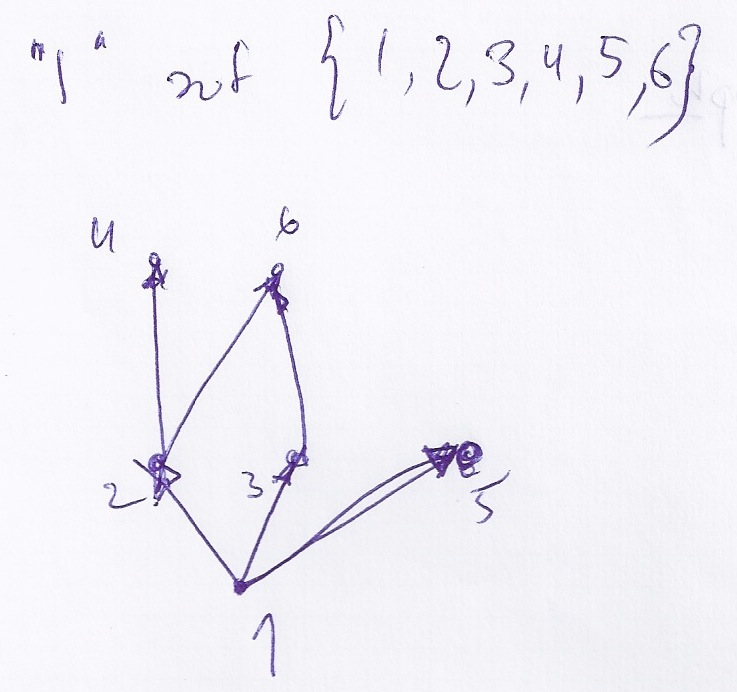
\includegraphics{Bild19} \\
			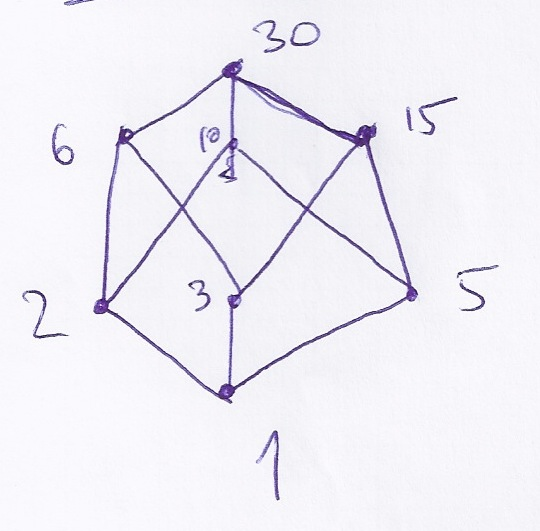
\includegraphics{Bild20}
		\item $\subseteq \text{ auf } \mathbb{P}( B ) \text{ für eine Menge } B$ \\
			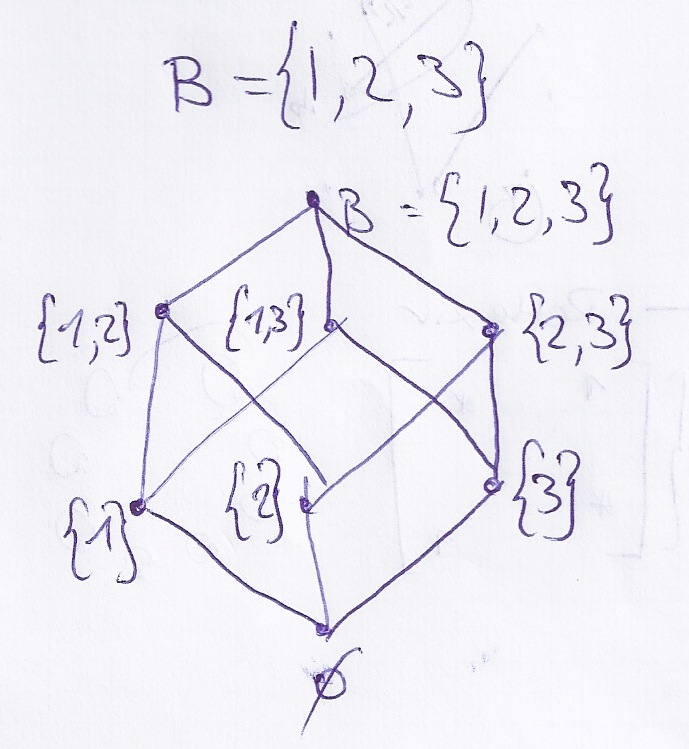
\includegraphics{Bild21}
	\end{itemize}
\end{bsp*}
\begin{bem}
	Nicht jedes Paar von Objekten muss vergleichbar sein.\\
	Falls es so ist, spricht man von einer \textbf{linearen}\index{Ordnung!lineare} oder \textbf{totalen}\index{Ordnung!totale} Ordnung, \textbf{Kette}\index{Kette}.
\end{bem}
\begin{def*}[note = vergleichbar , index = vergleichbar]
	$x$ und $y$ \textbf{vergleichbar}, falls $x \leq y \vee y \leq x$
\end{def*}

\subsubsection{Wichtige Begriffe}
\begin{def*}[note = maximales Element , index = Element!maximales]
	$x$ \textbf{maximales Element} falls \\
	\[ \not\exists y \neq x : y \geq x \qquad (\not\exists y : y > x) \qquad y > x :\iff y \geq x \wedge y \neq x \]
	analog: \textbf{minimales Element}\index{Element!minimales}
\end{def*}
\begin{def*}[note = grösstes Element , index = Element!grösstes]
	$x$ \textbf{grösstes Element} falls \\
	\[ \forall y \leq x \]
	analog: \textbf{kleinstes Element}\index{Element!kleinstes}
\end{def*}
\begin{def*}[note = wohlgeordnet , index = wohlgeordnet]
	$(A, \leq)$ heisst \textbf{wohlgeordnet (WO)} falls jede nichtleere Teilmenge ein kleinstes Element hat. \\
	\begin{bsp*}{wohlgeordnete Ordnungsrelation}
		\[ (\mathbb{N}, \leq ) \]
	\end{bsp*}
	\begin{bsp*}{keine WO}
		\begin{itemize}
			\item $(\mathbb{Z}, \leq )$
			\item $([0,1], \leq)$
		\end{itemize}
	\end{bsp*}
\end{def*}

\subsubsection{Hasse-Diagramme}
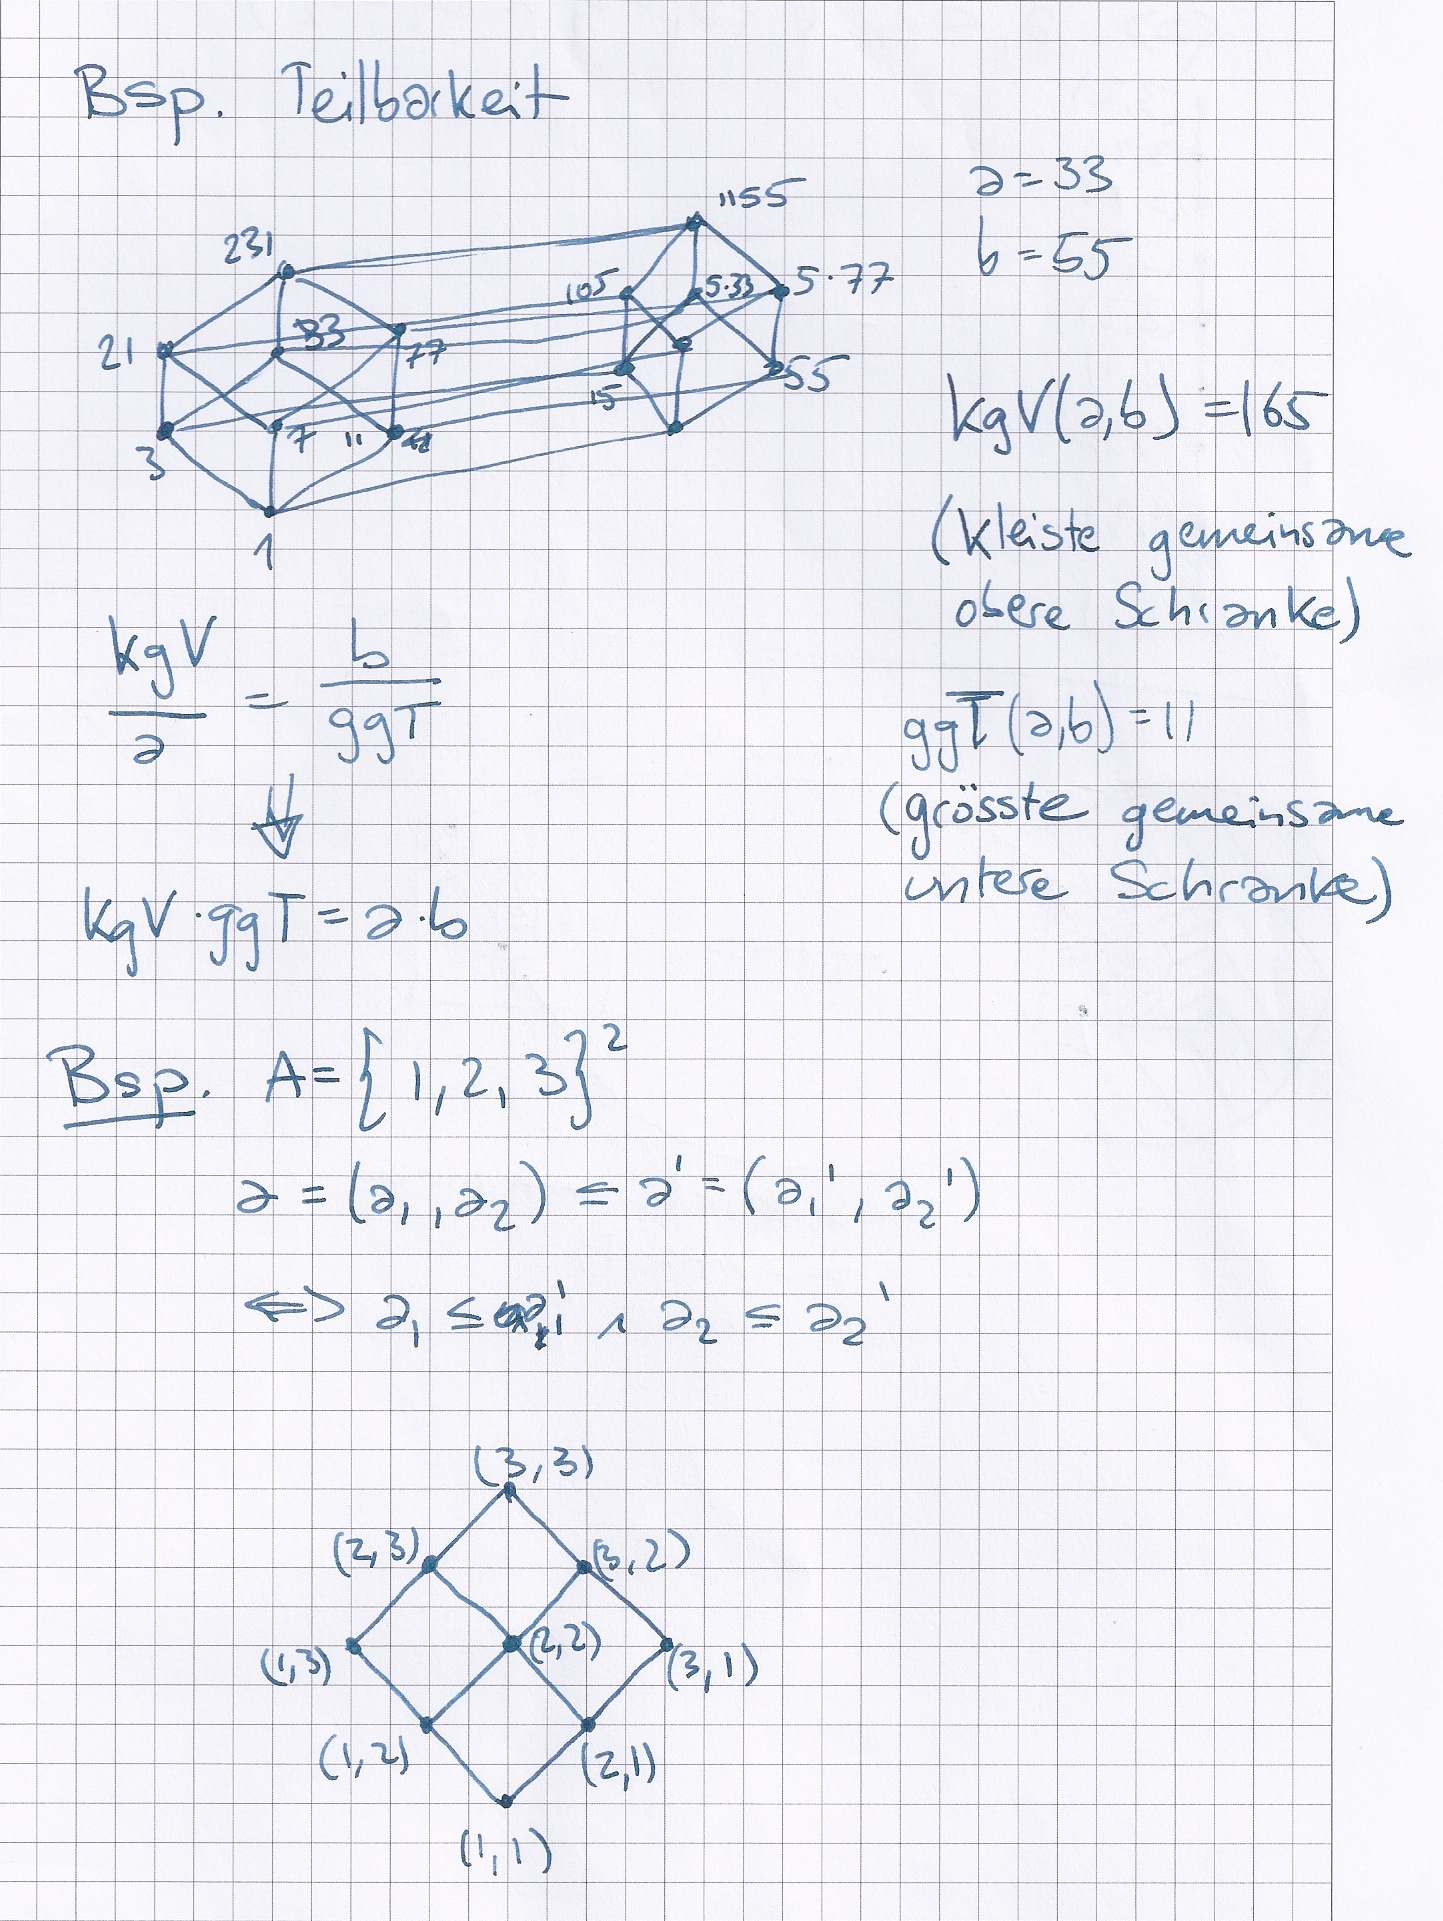
\includegraphics[width=\textwidth]{Bild22}
\begin{itemize}
	\item Es werden nur direkte Nachbarn verbunden $( x \leq y \text{ direkte Nachbarn }: x \neq y \wedge \not\exists z : x < z < y )$
	\item Orientierung durch Position ( unten $\leq$ oben )
\end{itemize}
\section{Funktionen}
\begin{def*}[note = Funktion , index = Funktion]
	Eine Relation $f \subseteq A \times B$ heisst \textbf{funktional} (Funktion $f: A \rightarrow B$) falls:
	\begin{gather*}
		\forall a \exists b : (a,b) \in f \\
		(a,b) \in f \wedge (a,b') \in f \implies b = b' \\
		\intertext{oder einfach:}
		\forall a \exists ! b (a,b) \in f
	\end{gather*}
	Wir schreiben für $(a,b) \in f$: \\
	$f( a ) = b , f: a \mapsto b$
\end{def*}
\begin{def*}[note = Komposition , index = Komposition]
	(Als Relationskomposition $''f \ring g''$) \\
	\begin{gather*}
		f: A \rightarrow B, g: B \rightarrow C \\
		g \ring f( a ) = g( f( a ))
	\end{gather*}
\end{def*}
\begin{def*}[note = Injektivität , index = Injektivität]
	$f: A \rightarrow B$ \textbf{injektiv}, falls \\
	$a \neq a \implies f( a ) \neq f( a' )$
\end{def*}
\begin{def*}[note = Surjektivität , index = Surjektivität]
	$f: A \rightarrow B$ \textbf{surjektiv}, falls \\
	$\forall b \exists a : f( a ) = b$
\end{def*}
\begin{def*}[note = Bijektivität , index = Bijektivität]
	$f: A \rightarrow B$ \textbf{bijektiv}, falls $f$ injektiv und surjektiv. \todo{Hyperref it up.}
\end{def*}

\subsubsection{Die Kardinalitäten von Mengen}
\begin{def*}[note = Gleichmächtig , index = Gleichmächtig]
	\begin{gather*}
		A \preceq B, \text{ falls } \exists f : A \rightarrow B \text{ injektiv } \iff \exists g : B \rightarrow A \text{ surjektiv}. \\
		A \approx B \text{ gleichmächtig, falls } \exists f : A \rightarrow B \text{ bijektiv}.
	\end{gather*}
	Dann gilt:
	\begin{itemize}
		\item $A \approx A \quad (f = id_A)$
		\item $A \preceq B \wedge b \preceq C \implies A \preceq C$
		\item $A \preceq B \wedge B \preceq A \implies A \approx B$
		\item Totalität: $A \preceq B \vee B \preceq A$
	\end{itemize}
\end{def*}
\begin{bsp*}
	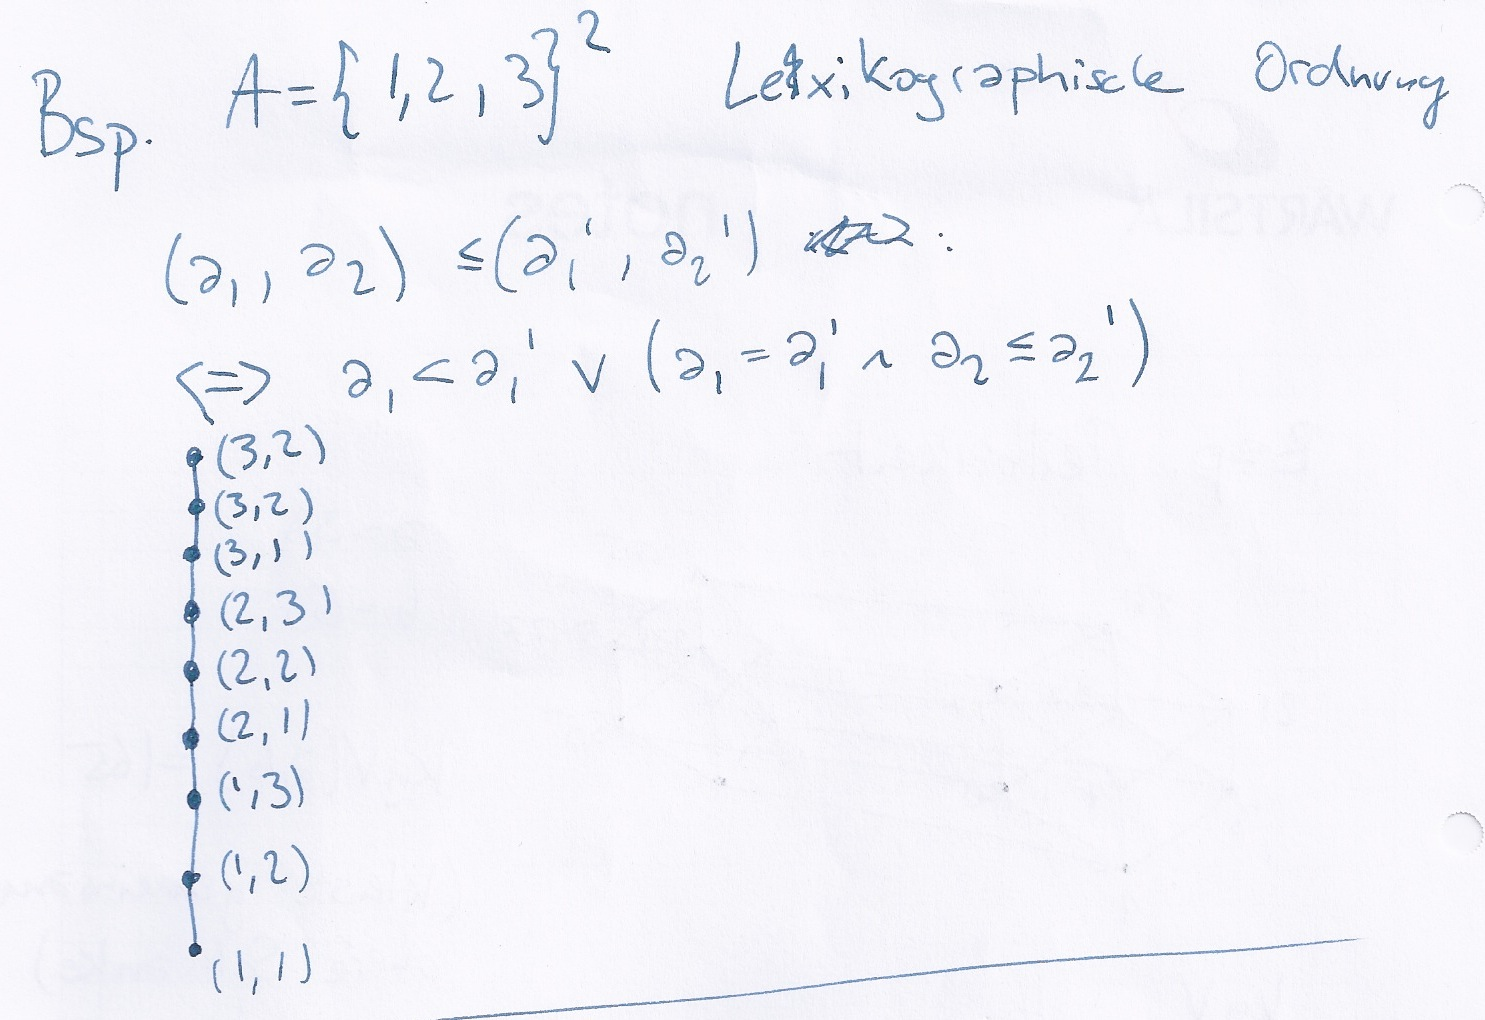
\includegraphics[width=\textwidth]{Bild23}
\end{bsp*}
\begin{satz*}[note = {(Schnöder, Bernstein, Cantor)}]
	$A \preceq B \wedge B \preceq A \iff A \approx B$\\
	\begin{bew}[note = ''Beweis'':]
		B hat eine zu A gleichmächtige Teilmenge und umgekehrt.\\
		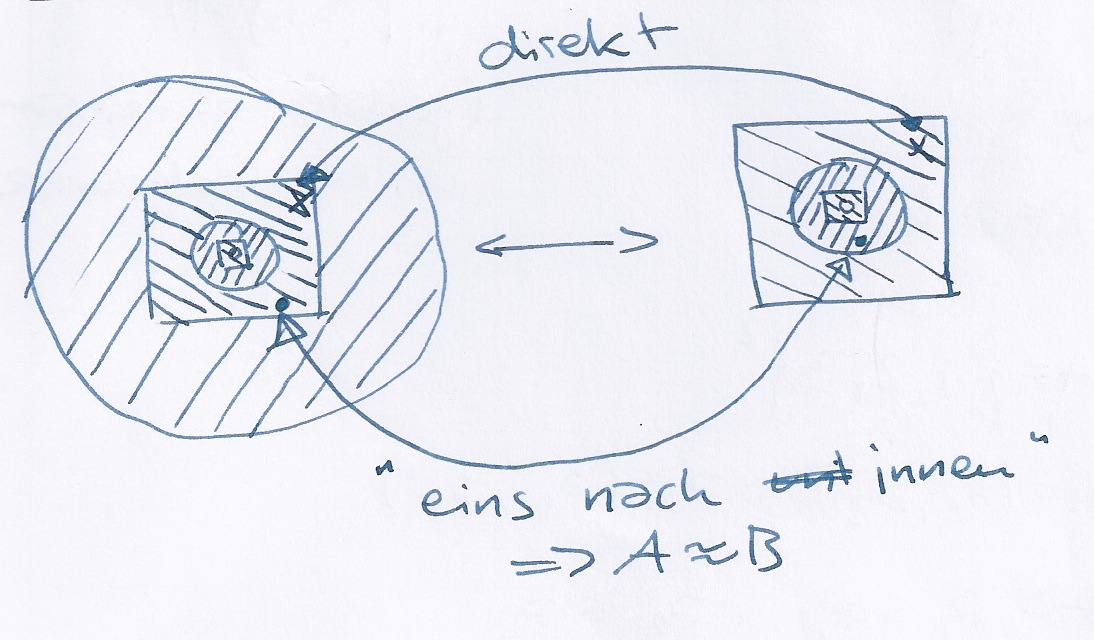
\includegraphics[width=\textwidth]{Bild24}
	\end{bew}
\end{satz*}
\begin{def*}[note = Gleichmächtigkeit , index = Gleichmächtigkeit]
	$\approx$ ist eine Äquivalenzrelation auf Klasse aller Mengen.\\
	Äquivalenklassen = Kardinalzahlen:\\
	$0, 1, 2, \dotsc , n, n+1, \dotsc \mathbb{N}, \dotsc , \mathbb{R}, \mathbb{P}(\mathbb{R}), \mathbb{P}(\mathbb{P}(\mathbb{R})), \dotsc$
\end{def*}
\begin{satz*}[note = (Cantor)]
	Für alle Mengen $A$ gilt\\
	\[ \mathbb{P}(A) \not\approx A \]
	\begin{bew}
		\begin{gather*}
			f: A \rightarrow \mathbb{P}(\mathbb{A}) \\
			\intertext{Wir zeigen: $f$ nicht surjektiv.}
			\forall a \in A : a \in f(a) \vee a \notin f(a) \\
			B \coloneqq \{ a \in A \mid a \notin f(a) \} \subseteq A, b \in \mathbb{P}(\mathbb{B}) \\
			\text{Annahme: } B = f(b) \\
				b \in B = f(b) ? \\
				b \in f(b) \implies b\notin f(b) \implies b \in f(b) \\
				\text{\lightning ~ Also } ( \not\exists f(b) = B ) \implies f \text{ nicht surjektiv } \blacksquare
		\end{gather*}
	\end{bew}
\end{satz*}

\chapter{Kombinatorik}
\section{Grundbegriffe}
\begin{bsp*}
	$u \cdot r$ Kästchen\\
	Auf wie viele Arten kann man auf kürzestem Weg von $A$ nach $B$?\\
	\begin{itemize}
		\item Ansatz 1: ''Divide et impera''
		\begin{gather*}
			\begin{array}{ l l }
				\text{Pascal-Dreieck:}		& \binom{n}{k} = \binom{n-1}{k-1} + \binom{n-1}{k}	\\
				\text{Verankerung:}		& \binom{n}{0} = \binom{n}{n} = 1					\\
				\text{Lösung:}			& \binom{u+r}{r}								
			\end{array}
		\end{gather*}
		\item Ansatz 2: Schnittfolge
		\begin{gather*}
			R_1 U_1 R_2 R_3 U_2 \dots U_u R_r \\
			\begin{array}{ l l }
				\text{\# Permutationen:}	& (u+r)!			\\
				\text{\# Wege:}			& \frac{(u+r)!}{u!r!}	
			\end{array}\\
			\intertext{Wir haben gesehen:}
			\binom{n}{k} = \frac{n!}{k!(n-k)!}
		\end{gather*}
	\end{itemize}
\end{bsp*}

\subsubsection{Interpretation von \texorpdfstring{$\binom{n}{k}$}{n tief k}}
\begin{itemize}
	\item Anzahl $k$-elementige Teilmengen einer $n$-Menge. \\
		\begin{bew}[note = {Direkter Beweis: Induktion über $n$}]
			\begin{gather*}
				n \rightarrow n+1 \\
				\# k\text{-Teilmengen einer } n+1\text{-Menge} \\
				\binom{n}{k} + \binom{n}{k-1} = \binom{n+1}{k}
			\end{gather*}
		\end{bew}
	\item Binomialkoeffizienten\\
		\[ (x+y)^n = \sum_{i=0}^n \binom{n}{i} x^i y^{n-i} \]
\end{itemize}

\subsubsection{''Urnenmodelle''}
\begin{bsp*}
	$n=3$ Kugeln\\
	Zeihe $k=3$ \\
	\begin{tabular}{ c | c c c | c c c }
								&\multicolumn{3}{c|}{geordnet}	&\multicolumn{3}{c}{ungeordnet}		\\	\hline
		\multirow{3}{*}{mit Zurücklegen}	& (1,1)	& (1,2)	& (1,3)	& (1,1)	& (1,2)	& (1,3)		\\
								& (2,1)	& (2,2)	& (2,3)	&		& (2,2)	& (2,3)		\\
								& (3,1)	& (3,2)	& (3,3)	&		&		& (3,3)		\\	\hline
		\multirow{3}{*}{ohne Zurücklegen}	&		& (1,2)	& (1,3)	&		& (1,2)	& (1,3)		\\
								& (2,1)	&		& (2,3)	&		&		& (2,3)		\\
								& (3,1)	& (3,2)	&		&		&		&				
	\end{tabular}\\ \phantom{.} \\
	\begin{tabular}{ l | l | l }
						& geordnet															& ungeordnet							\\	\hline
		mit Zurücklegen		& $n^k$ \footnote{Anzahle Wörter der Länge $k$ über einen Alphabet mit $n$ Zeichen}	& $\binom{n+k-1}{n} = \binom{n+k-1}{n-1}$ \footnote{\begin{gather*}
		\underbrace{1 2 3 1 1 2 1 3 2 3 \dots 3 2}_k \\
		\text{sortieren (kommt nicht drauf an, da ungeordnet)}\\
		\begin{array}{ c c c c c c c c c c c c c c c }
			1	&1	&1	&1	&\dots	&1	&|	&2	&2	&\dots	&2	&|	&3	&\dots	&3	\\
			*	&*	&*	&*	&\dots	&*	&|	&*	&*	&\dots	&*	&|	&*	&\dots	&*	
		\end{array}\\
		\left.\begin{array}{ l l l }
			\# \text{Anzahl}	& x	&: k	\\
			\# \text{Anzahl}	& |	&: n-1
		\end{array} \right\} \implies \binom{n+k-1}{n} = \binom{n+k-1}{n-1}
		\end{gather*}}	\\	\hline
		ohne Zurücklegen	& $\frac{n!}{(n-k)!} \eqqcolon n^{\underline{k}}$								& $\binom{n}{k}$						
	\end{tabular}
\end{bsp*}
\begin{bsp*}{\# Abstimmungsergebnisse}
	\begin{gather*}
		\underbrace{20 \text{ Stimmen}}_{k=20}, \underbrace{3 \text{ Varianten}}_{n=3} \\
		\binom{22}{20} = \binom{22}{2} = \frac{22 \cdot 21}{2} = 231
	\end{gather*}
\end{bsp*}

\section{Kombinatorische Regeln und Zählstrategien}
\subsubsection{Summenregel}
Falls $(A_i)_{i=1 \dots n}$ paarweise disjunkt $(i \neq j \implies A_i \cap A_j = \varnothing )$ dann \\
\[ \abs{\bigcup_{i=1}^n A_i} = \sum_{i=1}^n \abs{A_i} \]

\subsubsection{Produktregel}
\begin{gather*}
	(A_i)_{i=1 \dots n} \\
	\abs{\bigtimes_{i=1}^n A_i} = \prod_{i=1}^n \abs{A_i}
\end{gather*}

\subsubsection{Gleichheitsregel}
$S, T$ endlich, $\exists f: S \rightarrow T$ bijektiv $\implies \abs{S} = \abs{T}$

\subsubsection{Inklusion-Exklusion}
\begin{gather*}
	\abs{A_1 \cup A_2} = \abs{A_1} + \abs{A_2} - \abs{A_1 \cap A_2} \\
	\begin{split}
		\abs{A_1 \cup A_2 \cup A_3}
			&= \abs{A_1} + \abs{A_2} + \abs{A_3} \\
			&- \abs{A_1 \cap A_2} - \abs{A_1 \cap A_3} - \abs{A_2 \cap A_3} \\
			&+ \abs{A_1 + A_2 + A_3}
	\end{split}
	\intertext{$n$ Mengen:}
	\begin{split}
		\abs{A_1 \cup \dotsb \cup A_n}
			&= \bas{A_1} + \dotsb + \abs{A_n} \\
			&- \abs{A_1 \cap A_2} - \dotsb - \abs{A_{n-1} \cap A_n} \\
			&\vdots \\
			&+ (-1)^{n+1} \cdot \abs{A_1 \cap \dotsb \cap A_n}
	\end{split}\\
	\abs{\bigcup_{i=1}^n A_i} = \sum_{r=1}^n (-1)^{r-1} \sum_{1 \leq i_1 < i_2 < \dots < i_r \leq n} \abs{\bigcap_{j=1}^r A_{ij}} \\
	\abs{\bigcup_{i=1}^n A_i} = \sum_{k=1}^n (-1)^{k-1} \sum_{\substack{\text{alle } I \subseteq \{1,\dotsc,n\}\\\text{mit } \abs{I} = k}} \abs{\bigcap_{i \in I}^r A_{ij}} \\
\end{gather*}
\begin{bew}[note = Induktion über $n$]
	\begin{description}
		\item[IV)] $n=1 , n=2 \:\checkmark$
		\item[IS)] $n \rightarrow n+1$ \\
			\begin{align*}
				\abs{\bigcup_{i=1}^{n+1} A_i}
					&= \abs{(\bigcup_{i=1}^n A_i) \cup A_{n+1}} \\
					&= \abs{\bigcup_{i=1}^n A_i} + \abs{A_{n+1}} - \abs{(\bigcup_{i=1}^n A_i) \cap A_{n+1}} \\
					&= \underbrace{\sum_{r=1}^n (-1)^{r-1} \sum_{\substack{r\text{-Familien}\\a \leq i_j \leq n}} \abs{\bigcap_{j=1}^r A_{ij}}}_{r\text{-Familien ohne } A_{n+1}} + \underbrace{\abs{A_{n+1}}}_{1\text{-Familie } A_{n+1}} \\
					&\underbrace{ - \sum_{r=1}^n (-1)^{r-1} \sum_{r\text{-Familien}} \abs{\bigcap (A_i \cap A_n)}}_{+ \underbrace{\sum_{r=1}^n (-1)^{(r+1)-1} \sum_{r\text{-Familien}} \abs{\bigcap (A_i \cap A_n)}}_{(r+1) \text{ Familien mit } A_{n+1}}}
			\end{align*}
	\end{description}
\end{bew}
\subsubsection{Anwendungen}
Fixpunktfreie Permutationen\\
\[
\begin{pmatrix}
	1	& 2	& 3	\\
	2	& 3	& 1
\end{pmatrix} \qquad \begin{pmatrix}
	1	& 2	& 3	\\
	3	& 2	& 1
\end{pmatrix} \qquad
\begin{pmatrix}
	1	& 2	& \dots	& i	& i+1	& \dots	\\
	*	& *	& \dots	& i	& *	& \dots	
\end{pmatrix}
\]
Wie viele der $n!$ Permutationen einer $n$-Menge sind fixpunkte? \\
\begin{gather*}
	A_i \coloneqq \{ \text{Permutationen von } [n] \coloneqq \{1, 2, \dots, n \} \text{ mit Fixpunkt } i \} \\
	\begin{split}
	\text{\# Permutationen mit Fixpunkt}
		&= \abs{\bigcup_{i=1}^n A_i} \underset{\mathrm{I.-E.}}{=} \sum_{k=1}^n (-1)^{k-1} \sum_{\substack{I \subseteq \{1, \dotsc , n\}\\\abs{I} = k}} \underbrace{\abs{\bigcap A_{ij}}}_{(n-k)!} \\
		&= \sum_{k=1}^n (-1)^{k-1} \frac{n!}{k!} = n! - \frac{n!}{2!} + \frac{n!}{3!} - \frac{n!}{4!} + \dotsb
	\end{split} \\
	\begin{split}
	\text{\# fixpunktfreie } &= \frac{n!}{2!} -\frac{n!}{3!} +\frac{n!}{4!} \mp \dotsb \\
	&= n! ( 1 - \frac{1}{1!} +\frac{1}{2!} - \frac{1}{3!} + \frac{1}{4!} \mp \dots + (-1)^n \frac{1}{n!} ) \\
	&= n! ( 1 + \frac{(-1)}{1!} +\frac{(-1)^2}{2!} + \frac{(-1)^3}{3!} + \frac{(-1)^4}{4!} + \dots + \frac{(-1)^n}{n!} ) \\
	&\rightarrow \frac{1}{e}
	\end{split} \\
	e^x = 1 + \frac{x}{1!} +\frac{x^2}{2!} +\frac{x^3}{3!} + \dotsb
\end{gather*}

$\varphi(n) \coloneqq \abs{\{k \in \{0 , \dotsc , n-1 \} , ggT(k,n) = 1 \}}$ \\
Eulersche $\varphi$-Funktion.\\
\begin{bsp*}
	\begin{gather*}
		\begin{split}
			p,q \text{ prim}, p \neq q, \varphi(p \cdot q) &= p \cdot q  - q - p + 1 \\
			&= (p-1)(q-1) \\
			&= \varphi(p) \cdot \varphi(q) \quad \text{nur wenn $p,q$ prim!}
		\end{split} \\
		\text{Allgemein: } n = \prod_{i=1}^r {p_i}^{l_i} , l_i > 0 \text{ Primfaktorzerlegung} \\
		A_i = \{ \text{ durch $p_i$ teilbare Zahlen $0, \dotsc , n-1$} \} \\
		\abs{\bigcup_{i=1}^n A_i} = \sum_{r=1}^n (-1)^{r-1} \sum_{1 \leq i_1 < i_2 < \dots < i_r \leq n} \underbrace{\abs{\bigcap_{j=1}^r A_{ij}}}_{\substack{\text{Zahlen $0 \dots n-1$ geteilt von } \\p_{i_1} , p_{i_2} , \dotsc , p_{i_k} \\\implies \frac{n}{p_{i_1} \cdot p_{i_2} \cdot \dotsm \cdot p_{i_k}}}} \\
		\begin{split}
			\implies \varphi(n) &= n ( 1 - \sum_{k=1}^r (-1)^{k-1} \frac{1}{p_{i_1} \cdot p_{i_2} \cdot \dotsm \cdot p_{i_k}} ) \\
			&= n ( 1 + \sum_{p_{i_1} , \dotsc , p_{i_k}} (-\frac{1}{p_{i_1}}) \cdot (-\frac{1}{p_{i_2}}) \cdot \dotsm \cdot (-\frac{1}{p_{i_k}}) ) \\
			&= n \cdot (1-\frac{1}{p_{i_1}}) \cdot (1-\frac{1}{p_{i_2}}) \cdot \dotsm \cdot (1-\frac{1}{p_{i_k}})
		\end{split} \\
		\text{Also: } \varphi(n) = \prod_i {p_i}^{l_i} \cdot \prod_i \underbrace{(1- \frac{1}{p_i})}_{\frac{p_i-1}{p_i}}
	\end{gather*}
\end{bsp*}

\subsubsection{Diricheltsches Schubfachprinzip (DSFP)}
\begin{satz*}
	Wenn $n$ Objekte auf $k<n$ Schubfächer verteilt werden dann enthält mind. ein Schubfach mind. 2 Objekte.
	\begin{bew}
		Induktion über $k$ \\
		Verankerung: $k=1 \:\checkmark$ \\
		Schritt: $k \rightarrow k+1$: Falls höchstens ein Objekt im Schubfach 1: $n-1$ oder $n$ Objekte auf $k-1$ Schubfächer 
	\end{bew}
\end{satz*}
\begin{bsp*}
	$(1,17,5,3,20,2,4)$\\
	\begin{tabular}{ l l }
		monoton aufsteigende Teilfolge\index{Teilfolge!monoton aufsteigend}:	&$(1,5,20)$ \\
		monoton absteigende Teilfolge\index{Teilfolge!monoton absteigend}:	&$(17,4,3,2)$
	\end{tabular}\\
	Frage: Für eine Folge der Länge $n$, gibt es  eine untere Grenze für die Länge  der längsten \textbf{monoton} Teilfolge? \\
	Antwort: $\approx \sqrt{n}$\\
	Präzis: Eine Folge (unterschiedlicher Zahlen) der Länge $m^2 + 1$ hat eine monotone Teilfolge der Länge $m+1 \approx \sqrt{n}$
	\begin{bew}
		Indirekt: Annahme: Längste monotone Teilfolge hat Länge $\leq m$\\
		\[
			\begin{array}{ c c c c c c }
				a_1			& a_2				&a_3				& \dots	& a_{n-1}			& a_n		\\
				(\dots , \dots  )	& (\dots , \dots  )	& (\dots , \dots  )	& \dots	& (\dots , \dots  )	& (1,1)
			\end{array}
		\]
		(Länge der längsten aufsteigenden Teilfolge die mit $a_i$ beginnt, Länge der längsten absteigenden Teilfolge die mit $a_i$ beginnt)\\
		Einträge in $(\dots , \dots  ) : 1 \leq \dots \leq m$ \\
		Anzahl verschiedene $(\dots , \dots  ) \leq m^2$ \\
		DSFP: Zwei Paare müssen gleich sein: \\
		\[\begin{array}{ c c c c c }
			\dots		& a_i		& \dots	& a_j 		& \dots 	\\
					& (c,d)	&		& (c,d)	&		
		\end{array}\]
		\begin{tabular}{ l l }
			1. Fall:	& $a_i < a_j$ : aufsteigende Folge von $a_i$ der Länge $c+1 \:\lightning$ \\
			2. Fall:	& analog für $a_i > a_j$
		\end{tabular}
	\end{bew}
\end{bsp*}
\todo{Acronym: ref to the real stuff}

\subsubsection{Doppeltes Abzählen}
\[ \sum_{a \in A} m_a = \sum_{n \in B} n_b = \abs{S} \]
\begin{bsp*}
	\[\nu(n) \coloneqq \abs{\{ k> 0 : k \mid n \}} \]\\
	Frage: Was ist der Mittelwert von $\nu(k)$ für $k=1, \dotsc , n$ ? \\
	\[ \sum_{k=1}^n \nu(k) = \sum_{k=1}^n \mu(k) = \sum_{k=1}^n \left\lfloor \frac{n}{k} \right\rfloor \]
	\enquote{Jede $k$-te Zahl ist durch $k$ teilbar.} \\
	Wie gross ist das als Funktion von $n$? \\
	\begin{gather*}
		\sum_{k=1}^n \frac{n}{k} - n = \sum_{k=1}^n (\frac{n}{k} - 1) \leq \sum_{k=1}^n \left\lfloor \frac{n}{k} \right\rfloor \leq \sum_{k=1}^n \frac{n}{k} \\
		\left(\sum_{k=1}^n \frac{1}{k}\right) -1 \leq \underbrace{\frac{1}{n} \sum_{k=1}^n \left\lfloor \frac{n}{k} \right\rfloor}_{\frac{1}{n} \sum_{k=1}^n \mu(k)} \leq \sum_{k=1}^n  \frac{1}{k} \\
		\sum_{k=1}^n  \frac{1}{k} \geq \int_0^n \frac{1}{x+1} \:\mathrm{d}x = \ln(n+1) \geq \ln(x) \\
		\sum_{k=1}^n  \frac{1}{k} \leq \int_1^n \frac{1}{x} \:\mathrm{d}x+1 = \ln(n) +1
	\end{gather*}
\end{bsp*}

\section{Binomialkoeffizienten: Eigenschaften und Approximationen}
\begin{gather*}
	\binom{n}{k} = \frac{n!}{k!(n-k)!} = \frac{n\cdot (n-1) \dotsm (n-k+1)}{1 \cdot 2 \dotsm k}\\
	\binom{n}{k} = \binom{n}{n-k} \\
	\binom{n}{k} = \binom{n-1}{k-1} + \binom{n-1}{k}
\end{gather*}

\subsubsection{Vandermonde-Identität}
$n$ Kugeln, $r$ gelbe, $n-r$ blaue, zeihen $k$, davon $t$ gelb\\
\begin{gather*}
	\binom{n}{k} = \sum_{t=0}^k \binom{r}{t} \cdot \binom{n-r}{k-t}
\end{gather*}
\begin{satz*}[note = Binomialsatz , index = Binomialsatz]
	\[ (x+y)^n = \sum_{k=0}^n \binom{n}{k} x^{n-k} y^k \]
\end{satz*}
\begin{bsp*}
	\begin{gather*}
		x=1 \\
		y=1 \\
		2^n = \sum_{k=0}^n \binom{n}{k}
	\end{gather*}
\end{bsp*}
\begin{bsp*}
	\begin{gather*}
		x=1 \\
		y=-1 \\
		0 = \sum_{k=0}^n (-1)^k \binom{n}{k}
	\end{gather*}
	Konsequenz: Von einer best. Länge gibt es gleich viele Strings mit gerader und ungerader Parität, Parität von $s_1,s_2,\dotsc,s_n:$\\
	\[ \bigoplus_{i=1}^n s_i \]
\end{bsp*}

\subsubsection{Approximationen / Abschätzungen}
\begin{gather*}
	\begin{split}
		\binom{n}{k} &= \frac{n\cdot (n-1) \dotsm (n-k+1)}{1 \cdot 2 \dotsm k} \\
		&= \frac{n}{k} \cdot \frac{n-1}{k-1} \cdot \frac{n-2}{k-2} \dotsm \frac{n-i}{k-1} \dotsm \frac{n-(k-1)}{k-(k-1)} \geq \left( \frac{n}{k} \right)^k \\
		\frac{\binom{n}{k}}{\binom{n}{k}^k} &= \underbrace{\frac{n\cdot (n-1) \dotsm (n-k+1}{n^k}}_{\leq 1} \cdot \underbrace{\frac{k^k}{1 \cdot 2 \dotsm k}}_{=\frac{k^k}{k!} \leq e^k} \\
		\binom{n}{k} \leq e^k \cdot \left( \frac{n}{k} \right)^k = \left( \frac{n \cdot e}{k} \right)^k
	\end{split}\\
	\intertext{Exakter:}
	n! \approx \sqrt{2 \pi n} \binom{n}{e}^n \qquad \text{Stirling-Approximation} \\
	\intertext{Einsetzen:}
	\binom{n}{k} \approx \frac{\sqrt{2 \pi n} \binom{n}{e}^n}{\sqrt{2 \pi k} \binom{k}{e}^k \sqrt{2 \pi (n-k)} \binom{n-k}{e}^{n-k}} \\
	\frac{n^n}{k^k (n-k)^{n-k}} = \frac{1}{(\frac{k}{n})^k (\frac{n-k}{n})^{n-k}} = [(\frac{k}{n})^{\frac{k}{n}} (1 - \frac{k}{n})^{1-\frac{k}{n}}]^{-n}  \qquad x \coloneqq \frac{k}{n} \\
	= [x^x (1-x)^{1-x}]^n = 2^{n\overbrace{(-x\log_2 x - (1-x)\log_2 (1-x))}^{h(x)}} = 2^{n \cdot h( x )} = 2^{n \cdot h(\frac{k}{n})}
\end{gather*}

\subsubsection{Datenkompression}
Verlustfrei: gzip $\neq$ mpeg, jpeg \\
$n$ unfaire Münzwürfe \\
\begin{gather*}
	P(0) x > \frac{1}{2} \\
	\underbrace{\overbrace{000010000001000 \dots 0100}^n}_{\underbrace{1011100101110 \dots 0}_l}
\end{gather*}
Wie kurz kann $l$ sein?\\
Strings mit $\frac{n}{2}$ 0'er, $\frac{n}{2}$ 1'er: \\
\begin{gather*}
	P = x^{\frac{n}{2}} (1-x)^{\frac{n}{2}} \\
	\text{Anzahl: } \binom{n}{\frac{n}{2}} \approx 2^{n \overbrace{h(\frac{k}{n})}^{h(\frac{1}{2}) = 1}} = 2^n \\
	\intertext{Totale WSK:}
	2^n \cdot ( \sqrt{x(1-x)})^n = 2^n \cdot (<\frac{1}{2})^n = (<1)^n
\end{gather*}
Strings mit $xn$ 0'er, $(1-x)$ 1'er \\
\begin{gather*}
	P = x^{xn} (1-x)^{(1-x)n} = 2^{n(x \log_2 x + (1-x) \log_2 (1-x))} = 2 ^{-n \cdot h(x)} \\
	\text{Anzahl: } \binom{x}{xn} = 2^{n h(x)} \\
	\text{Totale WSK: } \approx 1
\end{gather*}
Codierbar durch einen String der Länge $n \cdot h(x)$ \\
\[ \underbrace{h(x)}_{-x \log_2 x -(1-x) \log_2 (1-x)}  \text{ misst den Informationsgehalt} \]
Allgemein: Quelle $x_i$ mit WSK $p_i$\\
\begin{gather*}
	\sum p_i = 1 \\
	H(X) = \sum_i -p_i \cdot \log_2 p_i
\end{gather*}
\section{Wichtige Spezielle Zählprobleme}
Äquivalenzrelationen. Wie viele Äquivalenzrelationen gibt es auf einer $n$-Menge? \\
Dasselbe: Wie viele Partitionen? \\
Einfacher: Wie viele Partitionen in $k ~(\leq n)$ Mengen? \\
\begin{gather*}
	S_{n,k} = S_{n-1,k_1}+ k \cdot S_{n-1,k} \\
	\begin{array}{ c c c c c c c c c }
		n=0	&1	&0	\\
		n=1	&0	&1	&0	\\
		n=2	&0	&1	&1	&0	\\
		n=3	&0	&1	&3	&1	&0	\\
		n=4	&0	&1	&7	&6	&1	&0	\\
		n=5	&0	&1	&15	&25	&10	&1	&0	\\
		n=6	&0	&1	&31	&90	&65	&15	&1	&0	\\
	\end{array} \text{ Sterling-Dreieck 2. Art}\index{Stirling-Dreieck!2. Art}
\end{gather*}

\subsubsection{Permutationen}
Permutation $\pi$ von $n$ Elementen: \\
\begin{gather*}
	\pi : \{ 1, 2, \cdots , n \} \rightarrow \{ 1, 2, \dotsc , n \} \text{ bijektiv} \\
	\begin{pmatrix}
		1		&2		&3		\dots		&n		\\
		\pi(1)		&\pi(2)	&\pi(3)	\dots		&\pi(n)
	\end{pmatrix}
\end{gather*}
\begin{bsp*}
	\begin{gather*}
		\begin{pmatrix}
			1	&2	&3	&4	&5	\\
			5	&4	&3	&2	&1	
		\end{pmatrix} \\
		1 \mapsto 5 \mapsto 1 \\
		2 \mapsto 4 \mapsto 2 \\
		3 \mapsto 3 \\
		\pi \text{ ist \textbf{selbstinvers, Involution}}
	\end{gather*}
\end{bsp*}

\subsubsection{Komposition:}
\begin{gather*}
	\begin{split}
		\begin{pmatrix}
			1	&2	&3	&4	&5	\\
			2	&4	&5	&3	&1	
		\end{pmatrix} \circ \begin{pmatrix}
			1	&2	&3	&4	&5	\\
			5	&1	&2	&4	&3
		\end{pmatrix} = \begin{pmatrix}
			1	&2	&3	&4	&5	\\
			1	&4	&3	&2	&5
		\end{pmatrix} \neq \\
		\neq \begin{pmatrix}
			1	&2	&3	&4	&5	\\
			1	&2	&4	&3	&5	
		\end{pmatrix} = \begin{pmatrix}
			1	&2	&3	&4	&5	\\
			5	&1	&2	&4	&3
		\end{pmatrix} \circ \begin{pmatrix}
			1	&2	&3	&4	&5	\\
			2	&4	&5	&3	&1	
		\end{pmatrix}
	\end{split} \\
	invpi = \begin{pmatrix}	 \todo{Add upsidedown pi with left harpoon leg}
		1	&2	&3	&4	&5	\\
		1	&2	&3	&4	&5
	\end{pmatrix} \text{ Identität } \pi \cdot invpi = \pi \\
	\pi = \begin{pmatrix}
			1	&2	&3	&4	&5	\\
			3	&1	&4	&5	&2	
	\end{pmatrix} \\
	\pi^{-1} = \begin{pmatrix}
			1	&2	&3	&4	&5	\\
			2	&5	&1	&3	&4	
	\end{pmatrix}
\end{gather*}

Regeln:
\begin{itemize}
	\item $\forall \pi_1 , \pi_2 , \pi_3 : ( \pi_1 \circ \pi_2 ) \circ \pi_3 = \pi_1 \circ ( \pi_2 \circ \pi_3 )$
	\item $\exists invpi \forall \pi : \pi \circ invpi = invpi \circ \pi = \pi$ Neutralelement
	\item $\forall \pi \exists \pi^{-1} : \pi \circ \pi^{-1} = \pi^{-1} \circ \pi = invpi$ Inverses
\end{itemize}
$\rightarrow$ Gruppe

Struktur einer Permutation?
\[
	\begin{pmatrix}
		1	&2	&3	&4	&5	&6	&7	&8	&9	&10	\\
		5	&9	&8	&10	&7	&6	&1	&3	&4	&2	
	\end{pmatrix}
\]
Jede Permutation lässt sich \textbf{eindeutig} (bis auf die Reihenfolge der Zyklen) in \textbf{disjunktive Zyklen} zerlegen.
\begin{gather*}
	(6) \circ \underbrace{(3,8)}_{=(8,3)} \circ \underbrace{(1,5,7)}_{\substack{=(7,1,5)\\=(5,7,1)}} \circ (2,9,4,10) \\
	\pi = \begin{pmatrix}
		1	&2	&3	&4	&5	&6	&7	&8	&9	&10	\\
		10	&3	&6	&1	&4	&7	&2	&8	&5	&9	
	\end{pmatrix}\\
	\pi = (8)(1,9,4,10,5)(2,3,6,7) \\
	\pi^{20} = invpi \\
	\pi^2 = (8)(1,9,4,10,5)(2,6)(3,7)
\end{gather*}
Zählen: $S_{n,k} = $ \# Permutationen von $n$ Elementen mit genau $k$ Zyklen.
\begin{gather*}
	S_{0,0} \coloneqq 1 \\
	S_{n,0} = 0 \:(n \geq 1) \\
	S_{n,k} = 0 \:(k > n) \\
	S_{n,n} = 1 (invpi)
	\intertext{Rekursiongleichung}
	S_{n,k} = S_{n-1,k-1} + (n-1) S_{n-1,k}
\end{gather*}

\subsubsection{Stirling-Dreieck 1. Art}\index{Stirling-Dreieck!1. Art}
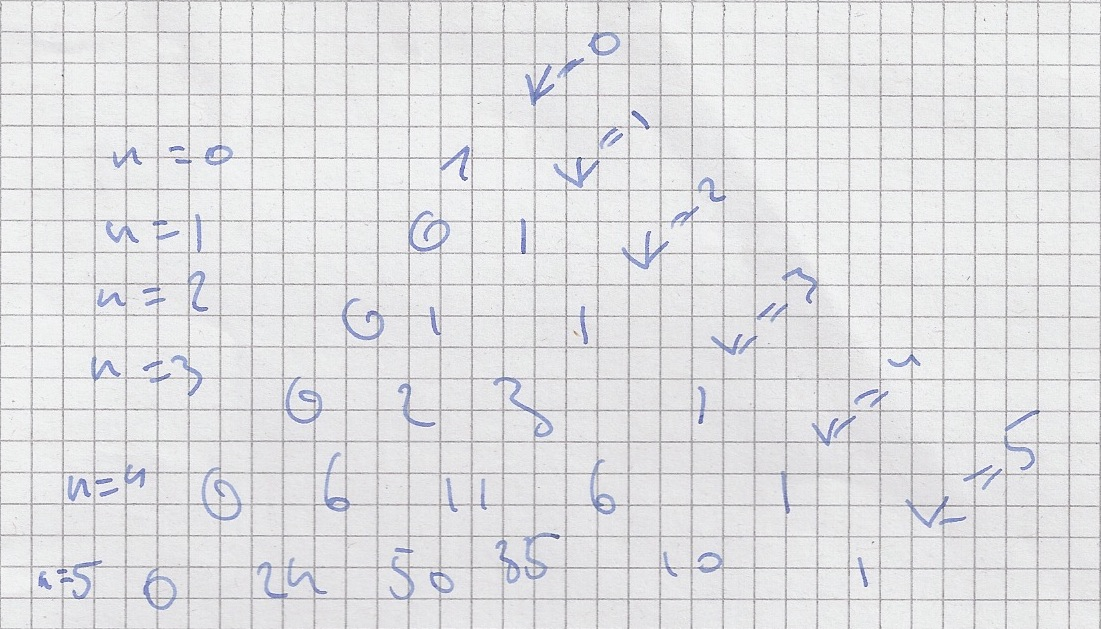
\includegraphics{Bild25}

\subsubsection{Partition von Zahlen}
Auf wie viele Arten kann eine Zahl $n \in \mathbb{N}$ als Summe $n = n_1 + n_2 + \dots + n_k$ von \textbf{positiven} ganzen Zahlen. Wir unterscheiden geordnet / ungeortdnet.
\begin{gather*}
	4 = \left\{ \begin{matrix}
		1	&+	&3	\\
		2	&+	&2	\\
		3	&+	&1	
	\end{matrix} \right. \qquad 4= \left\{ \begin{matrix}
		1	&+	&3	\\
		2	&+	&2	
	\end{matrix} \right.
	\intertext{Ungeordnet:}
	P_{n,k} \\
	\begin{matrix}
		k > n :	& P_{n,k} = 0 \\
		n \geq 1 :	& P_{n,0} = 0 \\
				& P_{0,0} \coloneqq 1 \\
				& P_{n,n} = 1 \\
				& P_{n,1} = 1
	\end{matrix} \\
	\intertext{Rekursion?}
	n > k : n \text{ mit } k \text{ Summanden } \rightarrow n-k \text{ mit } k-i \text{ Summanden } (0 \leq i \leq k-1) \\
	P_{n,k} = \sum_{i=1}^k P_{n-k,i}
	\intertext{Geordnet}
	n = \overbrace{\underbrace{1+1+1}_{n_1} \oplus \underbrace{1+\dots}_{n_2} \oplus \dots \oplus \underbrace{+1}_{n_k}}^n \\
	\binom{n-1}{k-1}
\end{gather*}
Anzahl Möglichkeiten, $n$ als Summe positiver Summanden zu schreiben?
\[ \sum_{k=1}^n \binom{n-1}{k-1} = \sum_{k'=1}^{n-1} \binom{n-1}{k'} = 2^{n-1} \qquad \text{Jedes + unabhängig} \]

\section{Lösen von Rekursionsgleichungen}
\begin{bsp}[note = Fibonacci-Folge , index = Fibonacci-Folge]
	\begin{gather*}
		f_n = f_{n-1} + f_{n-2} \qquad (n>1) \\
		f_0 = 0 \\
		f_1 = 1 \\
		\text{Explizite Darstellung } f_n = \dots \\
		\text{Ansatz: } f_n = \lambda^n \\
		\lambda^n = \lambda^{n-1} + \lambda^{n-2} \\
		( \lambda^2 - \lambda - 1 ) \lambda^{n-2} = 0 \qquad | \lambda \neq 0 \\
		\intertext{Charakteristisches Polynom}
		\lambda^2 - \lambda + 1 = 0 \\
		\lambda_{1,2} = \frac{1 \pm \sqrt{1+4}}{2} = \frac{1 \pm \sqrt{5}}{2} \\
		\text{Zwei Lösungen: } \lambda_1^n , \lambda_2^n . \\
		f_{a,b}(n) = a \cdot \lambda_1^n + b \cdot \lambda_2^n \\
		\text{Beh.: } f_{a,b}(n) \text{ ist die Lösung der Rekursion} \\
		\begin{split}
		f_{a,b}(n)	&= a \cdot \lambda_1^n + b \cdot \lambda_2^n \\
				&= a ( \lambda_1^{n-1} + \lambda_1^{n-2} ) + b ( \lambda_2^{n-1} + \lambda_2^{n-2} )	\\
				&= a \lambda_1^{n-1} + b \lambda_2^{n-1} + a \lambda_1^{n-2} + \lambda_2^{n-2} \\
				&= f_{a,b}(n-1) + f_{a,b}(n-2)
		\end{split}
		\intertext{Bestimmung von $a,b$ mit Randbedingungen}
		0 = a \underbrace{\left( \frac{1+\sqrt{5}}{2} \right)^0}_1 + b  \underbrace{\left( \frac{1-\sqrt{5}}{2} \right)^0}_1 \implies a = -b \\
		1 = (-b) \left( \frac{1+\sqrt{5}}{2} \right)^1 + b \left(  \frac{1-\sqrt{5}}{2} \right)^1 \\
		1 = -b \sqrt{5} \\
		b = -\frac{1}{\sqrt{5}} , a = \frac{1}{\sqrt{5}} , f_n = \frac{1}{\sqrt{5}} \left( \left( \frac{1+\sqrt{5}}{2} \right)^n - \left( \frac{1-\sqrt{5}}{2} \right)^n \right) \\
		|\lambda_2| < 1 \\
		f_n \approx \frac{1}{\sqrt{5}} \left( \underbrace{\frac{1+\sqrt{5}}{2}}_\lambda \right)^n \\
		\lambda \text{ ist Lösung von } \lambda^2 - \lambda +1 = 0 \\
		\lambda^2 = \lambda + 1 \\
		\frac{\lambda}{1} = \frac{\lambda + 1}{\lambda} \qquad \textbf{Goldener Schnitt}\index{goldener Schnitt}
	\end{gather*}
\end{bsp}
\todo{Too long}
\begin{bsp}
	\begin{gather*}
		g_n = 6 g_{n-1} - 12 g_{n-2} + 8 g_{n-3} \\
		g_0 = 1 \\
		g_1 = 2 \\
		g_2 = 3 \\
		\underbrace{\lambda^3 - 6 \lambda^2 + 12 \lambda - 8}_{=(\lambda-2)^3} = 0 \\
		\text{Lösungen: } 2^n , n \cdot 2^n , n^2 \cdot 2^n \\
		\intertext{Verifikation:}
		n \cdot 2^n \overset{?}{=} 6 (n-1) 2^{n-1} - 12 (n-2) 2^{n-2} + 8 (n-3) 2^{n-3} \\
		n \cdot 8 \overset{?}{=} 6(n-1)4 - 12(n-2)2 + 8(n-3) \\
		8n \overset{?}{=} 24n - 24 -24n +48 +8n -24 \quad \checkmark \\
		\intertext{Allgemeine Lösung:}
		g_n = a \cdot 2^n + b \cdot n \cdot 2^n + c \cdot n^2 \cdot 2^n \\
		\intertext{Sepezielle Lösung:}
		1 = a \\
		2 = 2a + 2b + 2c  \implies b = -c \\
		3 = 4a + 8b + 16c \implies 3 = 4+ 8c \\
		c = -\frac{1}{8} , b = \frac{1}{8} \\
		g_n = 2^n + \left( \frac{n - n^2}{8} \right) \cdot 2^n
	\end{gather*}
\end{bsp}
\begin{bsp}
	\begin{gather*}
	\underbrace{\overbrace{\Box}^{\frac{n}{2}} \overbrace{\Box}^{\frac{n}{2}}}_n * \underbrace{\overbrace{\Box}^{\frac{n}{2}} \overbrace{\Box}^{\frac{n}{2}}}_n \qquad \text{Divide et impera} \\
	T(n) = 4 \cdot T\left(\frac{n}{2}\right) \\
	T(1) = t_0\\
	\text{Substitution: } n =2^m \qquad m = \log_2 n \\
	T(2^m) = 4 \cdot T(2^{m-1}) \\
	S(m) = 4 \cdot S(m-1) \\
	\intertext{Löse $S$}
	\text{Char. Pol.: } \lambda - 4 = 0 \\
	\text{Allg. Lösung: } S(m) = a \cdot 4^m \\
	T(n) = S(\overbrace{\log_2 n}^m) = a \cdot 4^{\log_2 n} = a \cdot n^2 \\
	\text{Spez. Lösung: } T(n) = t_0 \cdot n^2
	\end{gather*}
\end{bsp}
$\Bigg[$Karatsuba\index{Karatsuba}: Es braucht nur 3 Mult.
\begin{gather*}
	T(n) = 3 \cdot T\left(\frac{n}{2}\right) \\
	\text{Ansatz: } T(n) = n^x \\
	\text{Einsetzen: } n^x = 3\left(\frac{n}{2}\right)^x \implies 3 =2^x \implies x = \log_2 3 \quad (<2) \\
	a \cdot b = a_1 b_1 K^2 + \underbrace{a_1 b_2 K + a_2 b_1 K}_{\underbrace{(a_1 b_2 + a_2 b_1)}_{\substack{(a_1 + a_2)(b_1 + b_2)\\ = a_1 b_1 + (a_1 b_2 + a_2 b_1) + a_2 b_2}}K} + a_2 b_2
\end{gather*}
Dimension\index{Dimension}:
\begin{gather*}
	\begin{matrix*}[l]
		\text{dim } 1:	&V(l) = l	\\
		\text{dim } 2:	&V(l) = l^2	\\
		\text{dim } 3:	&V(l) = l^3	
	\end{matrix*}\\
	V(l) = 4 V\left(\frac{l}{3}\right) \\
	l^d = 4 \cdot \left(\frac{l}{3} \right)^d \\
	3^d = 4 \\
	d = \log_3 4
\end{gather*}
$\Bigg]$\\
\begin{bsp}
	\begin{gather*}
		h(0) = 0 \\
		h(1) = 2 \\
		h(n) = 2h(n-1) - 2h(n-2) \\
		\text{Char. Pol.: } \lambda^2 - 2\lambda + 2 = 0 \\
		\lambda_{1,2} = \frac{2 \pm \sqrt{4-8}}{2} = 1 \pm i \\
		\text{Allg. Lös.: } a(1+i)^n + b(1-i)^n \\
		\text{Spez. Lös.: } 0 = a(1+i)^0 + b(1-i)^0 \implies b = -a \\
		2 = a(1+i) + (-a)(1-i) = 2ai \implies a = \frac{1}{i} = -i \\
		h(n) = \frac{1}{i} [(1+i)^n - (1-i)^n] \in \mathbb{N}
	\end{gather*}
\end{bsp}
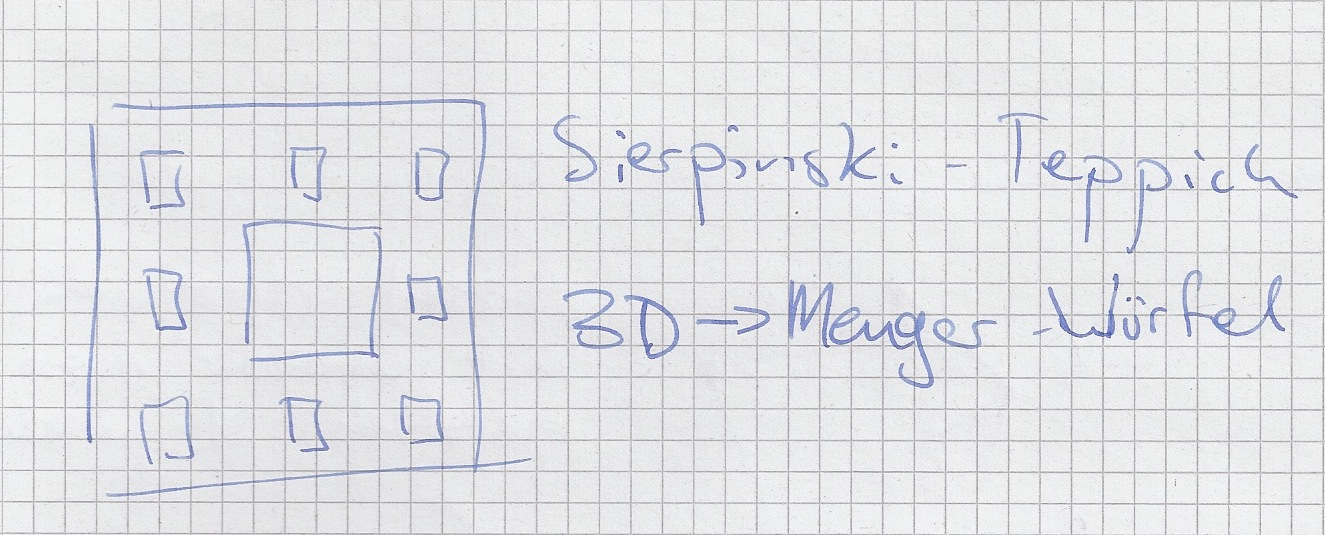
\includegraphics{Bild26} \\
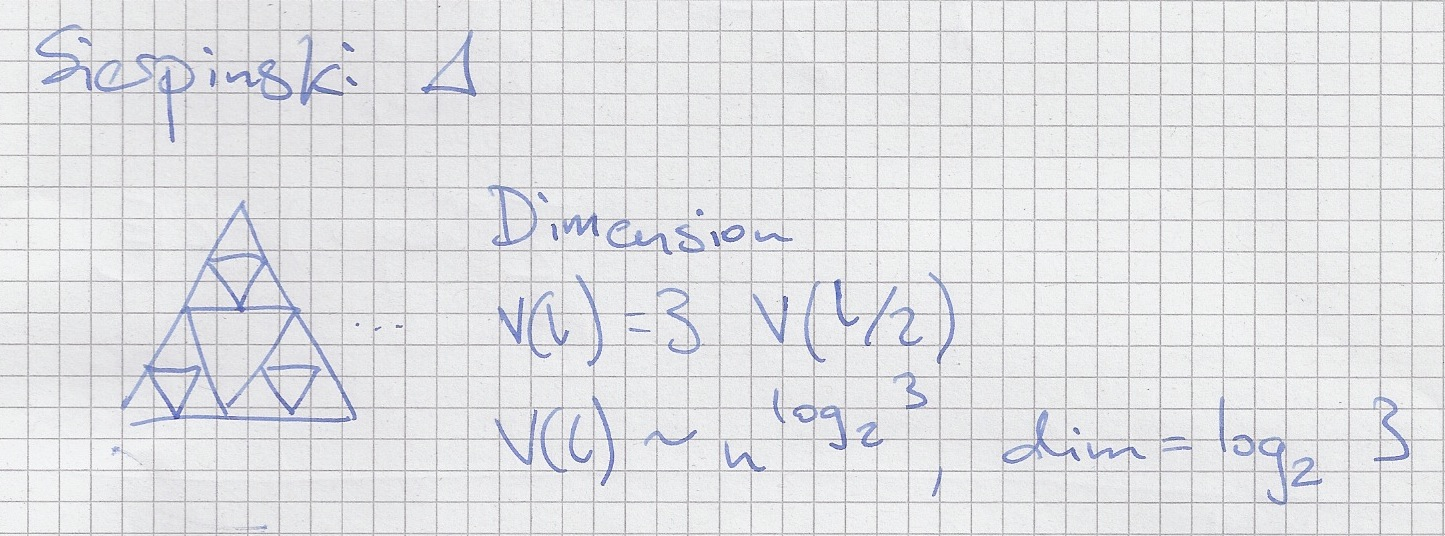
\includegraphics{Bild27}
\chapter{Graphentheorie}
\section{Motivation}
Vieles vom Gesehenen sind Graphen.
\subsubsection{Hasse-Diagramme}
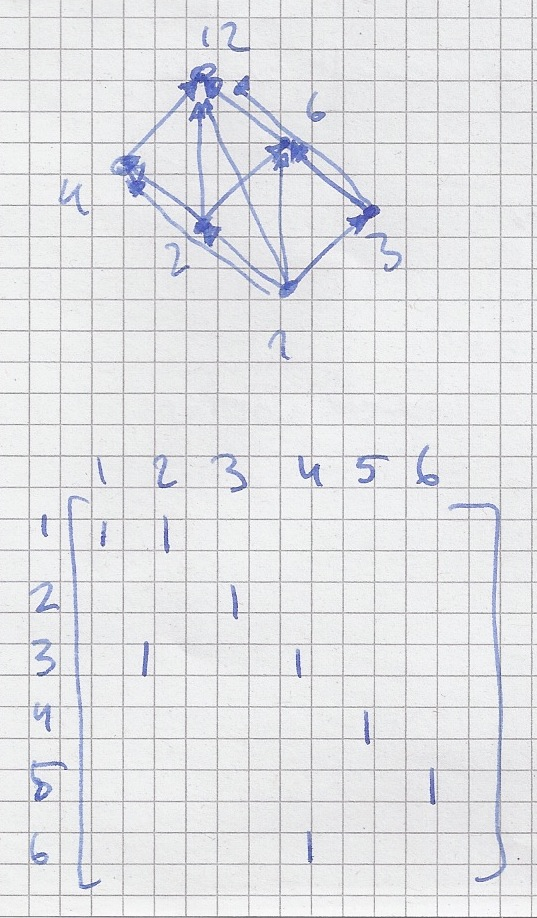
\includegraphics{Bild28} \\
Adjazenzmatrix des Graphen
\subsubsection{Relationen}
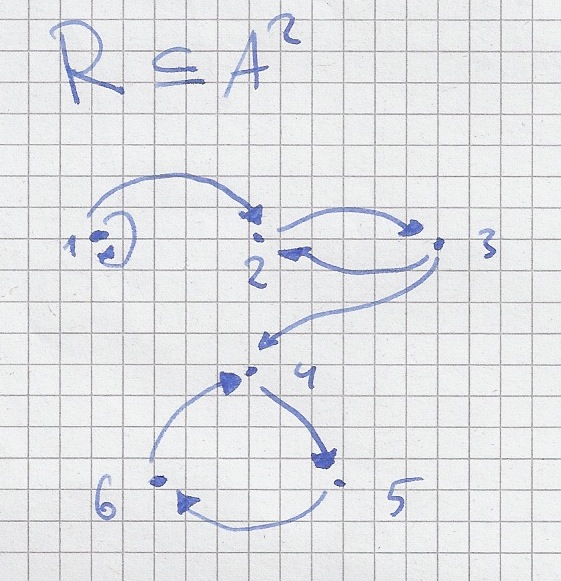
\includegraphics{Bild29} \\
\begin{bsp*}
	Gläser anstossen \\
	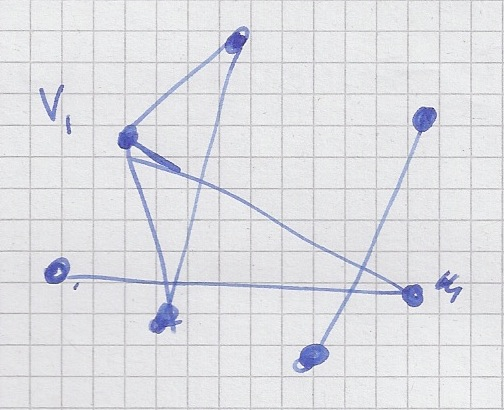
\includegraphics{Bild30} \\
	Anzahl derer, die mit ungerader Anz. anstossen, ist gerade.
	\begin{gather*}
		\deg(v_1) = 3 \\
		\sum_i \deg(v_i) = 2\underbrace{|E|}_{\substack{Anz.\\Kanten}} \\
		|\{i | \deg(v_i) \text{ ungerade}\}| \text{ gerade}
	\end{gather*}
\end{bsp*}
\begin{bsp*}[note = Fehlerfreie Kommunikation über verrauschte Kanäle]
	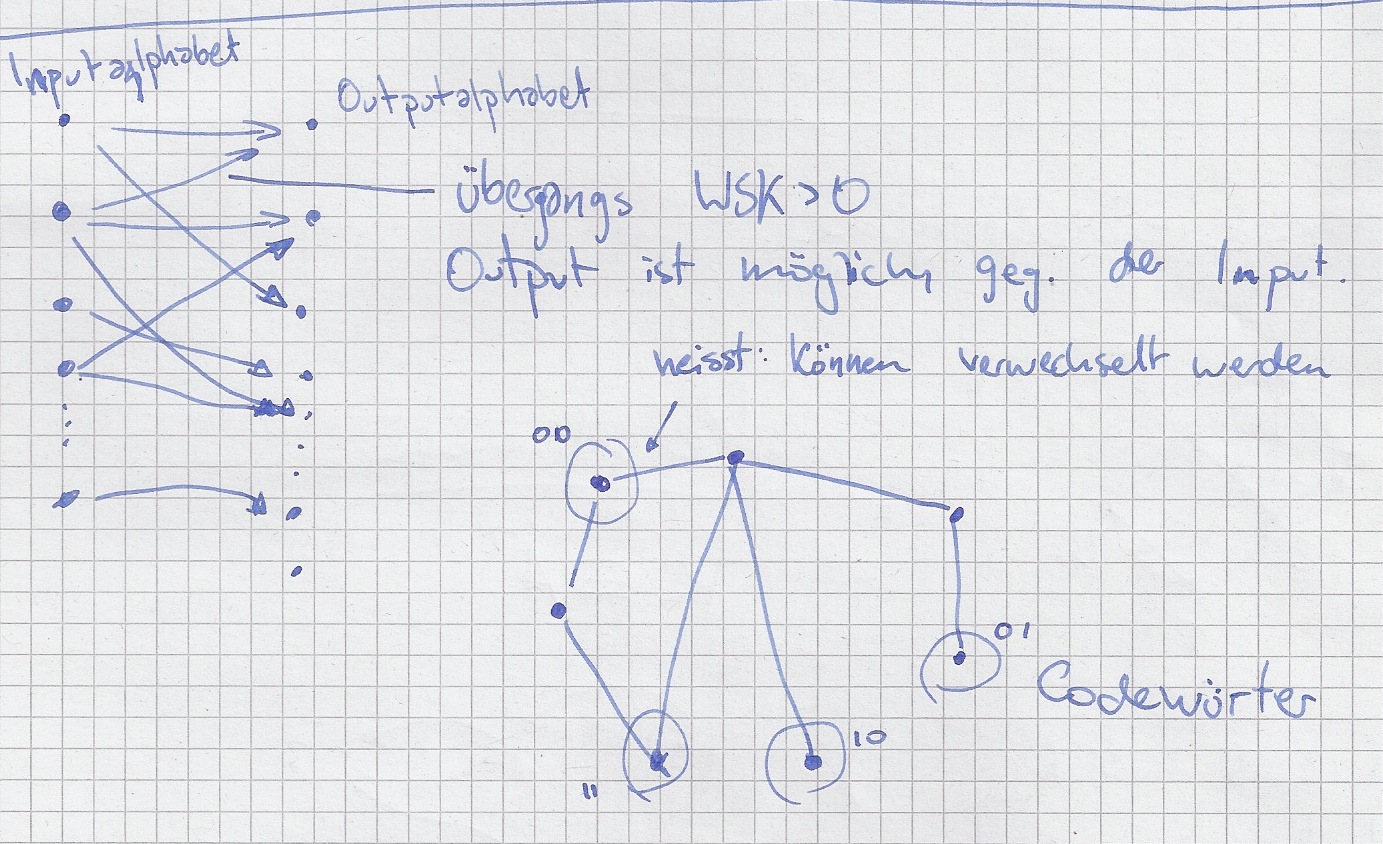
\includegraphics[width=\textwidth]{Bild31}
\end{bsp*}
\subsubsection{Konkreter Kanal(Shannon, 1948)}
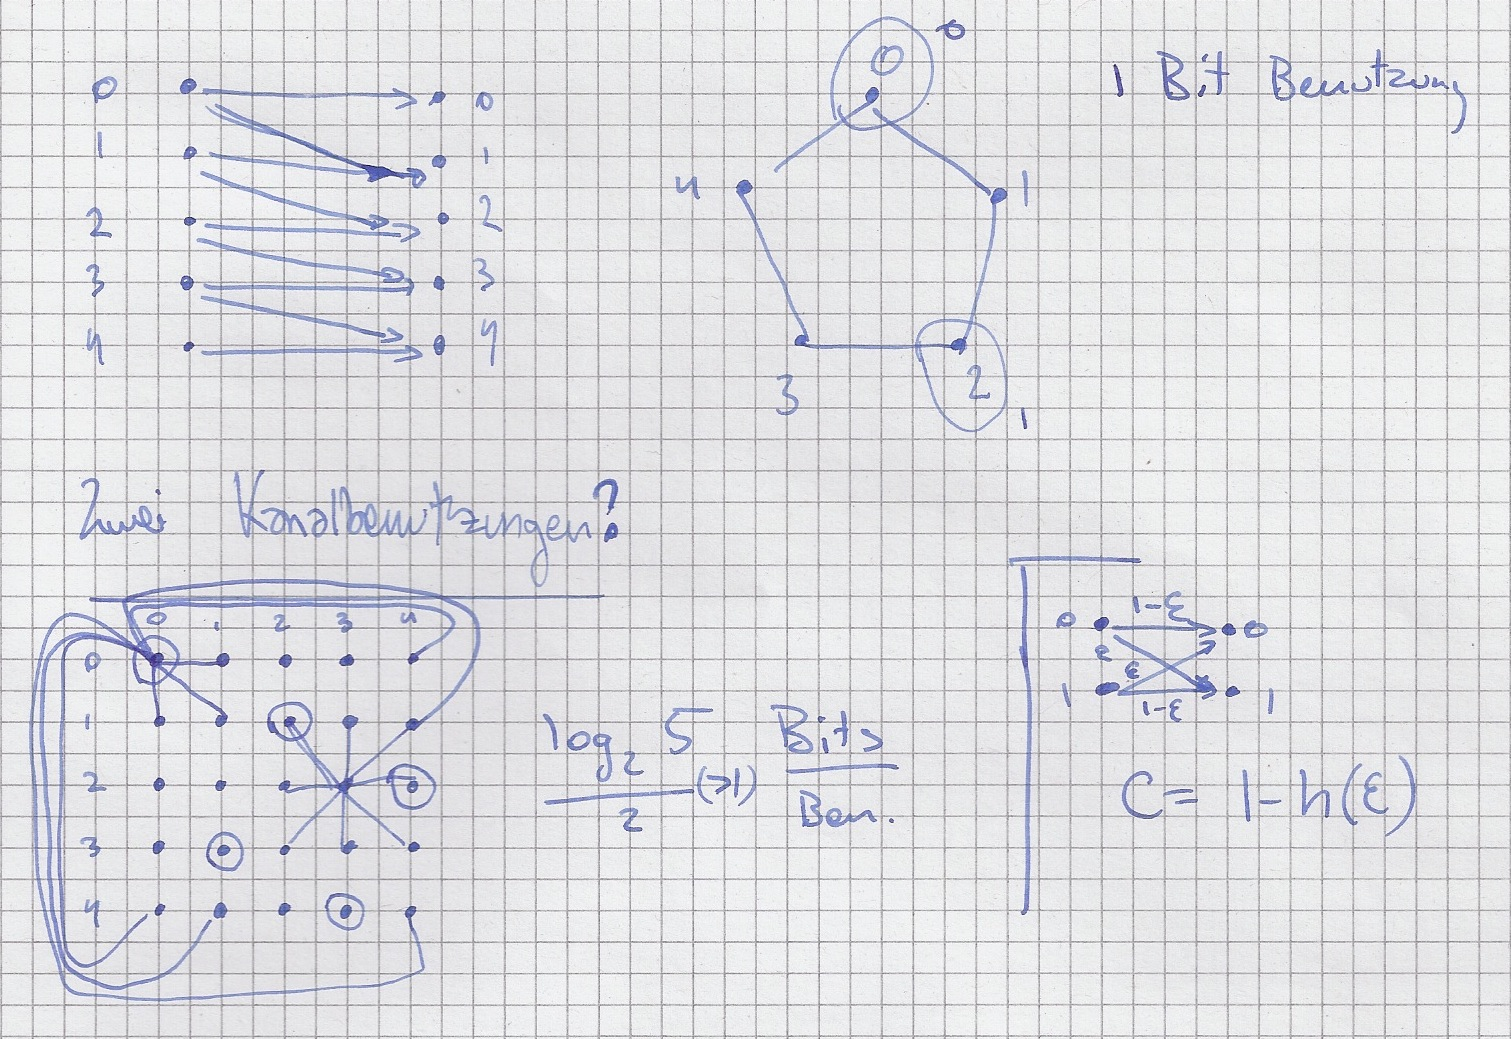
\includegraphics[width=\textwidth]{Bild32}

\section{Grundbegriffe}
\begin{def*}[note = Graph , index = Graph]
Graph $G = (V,E)$ \\
$V$ Menge, $0 < |V| < \infty$ (Knoten) \\
$E$ Relation auf $V, E \subseteq V^2$ (Kanten) \\
$G$ \textbf{ungerichtet}\index{Graph!ungerichtet}, falls $(u,v) \in E \iff (v,u) \in E$\\
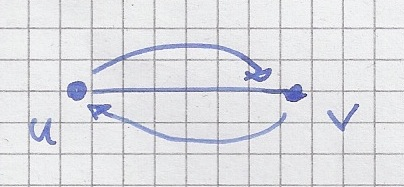
\includegraphics{Bild33} \\
Man schribt manchmal für ungerichtete $E \subseteq \{ \{u,v\} | u \neq v \}$\\
$\Gamma(v) \coloneqq \{ w \in V | (v,w) \in E \}$ \textbf{Nachbarschaft}\index{Nachbarschaft} \\
$\deg^-(v):$ Eingangsgrad\index{Grad!Eingangsgrad} \\
$\deg^+(v):$ Ausgangsgrad\index{Grad!Ausgangsgrad} \\
\[ \sum_N \deg^-(v) = \sum_N \deg^+(v) = |E| \]
Ungerichtet:
\[ \sum_N \deg(v) = 2|E| \]
$G$ \textbf{einfach}\index{Graph!einfach}, falls es keine \textbf{Loops} und keine \textbf{Mehrfachkanten}.
\end{def*}

\subsubsection{Grundbegriffe für einfache ungerichtete Graphen}
\begin{def*}[note = Weg , index = Weg]
$W = ( v_0 , \dotsc , v_l ) ; (v_i,v_{i+1}) \in E \quad \forall i = 0 , \dotsc , l-1$ (auch $v_0$-$v_l$-Weg ) $(l > 0)$
\end{def*}
\begin{def*}[note = Pfad , index = Pfad]
Weg, bei dem alle Knoten paarweise verschieden sind. ($v_0$-$v_l$-Pfad )
\end{def*}
\begin{def*}[note = zusammenhängend , index = Graph!zusammenhängend]
	$G=(V,E)$ zusammenhängend, falls $\forall u , v \in V \exists u$-$v$-Pfad
\end{def*}
\begin{def*}[note = Kreis , index = Kreis]
	$C=(v_1 , \dotsc , v_l)$, paarweise verschieden, $(v_i,v_{i+1}) \in E \forall i = 1 , \dotsc , l-1 \wedge (v_l , v_1) \in E \quad (l \geq 3 )$
\end{def*}
\begin{def*}[note = Teilgraph , index = Teilgraph]
	$H=(V',E')$ Teilgraph von $G=(V,E)$ falls $V' \subseteq V$ und $E' \subseteq V' \times V'$ und $E' \subseteq E$.
\end{def*}
\begin{def*}[note = induzierter Teilgraph , index = Teilgraph!induzierter]
	$H'$ von $V'$ induzierte Teilgraph, falls $\forall u , v \in V' : (u,v) \in E \implies (u,v) \in E'$. Wir schreiben $H'=G[V']$
\end{def*}
\begin{def*}[note = Zusammenhangskomponente , index = Zusammenhangskomponente]
	$G=(V,E) , (V_i)$ Partition von $V$ so, dass $\exists u$-$v$-Pfad $\iff \exists i : u \in V_i \ni v$. Dann $G[V_i]$ Zusammenhangskomponente von $G$.
\end{def*}
\begin{def*}[note = Brücke , index = Brücke]
	$e \in E$ Brücke falls $G'=(V,E \setminus \{e\})$ eine Zusammenhangskomponente mehr hat als $G$.
\end{def*}
\begin{satz*}
	$G=(V,E)$ hat mindestens $|V|-|E|$ Zusammenhangskomponenten
	\begin{bew}
		$G=(V,\varnothing)$ hat |V| Zusammenhangskomponenten. Jede Kante $e$, diehinzugefügt wird, reduziert ihre Anzahl höchstens um $1$.
	\end{bew}
	\begin{korr*}
		$G$ zusammenhängend $\implies |V| - |E| \leq 1$
	\end{korr*}
\end{satz*}
\section{Bäume}
\begin{def*}[note = Wald , index = Wald]
	Ein ungerichteter, einfacher Graph \textbf{ohne Kreise} heisst \textbf{Wald}.
\end{def*}
\begin{def*}[note = Baum , index = Baum]
	Ein Zusammenhängender Wald heisst \textbf{Baum}.
\end{def*}
\begin{def*}[note = Blatt , index = Blatt]
	Ein $v \in V$ mit $\deg(v) = 1$ heisst Blatt.
\end{def*}
\begin{satz*}
	Jeder Baum (mit $|V| \geq 2$) hat mindestens zwei Blätter.
\end{satz*}
\begin{satz*}
	Folgende Aussagen sind äquivalent: $G=(V,E)$ einfacher Graph.
	\begin{enumerate}
		\item $G$ ist ein Baum (zusammenhängend und kreislos)
		\item $G$ ist zusammenhängend, $|V| = |E| + 1$
		\item $G$ ist kreislos, $|V| = |E| + 1$
		\item $G$ ist zusammenhängend, jede $e \in E$ ist Brücke
		\item $G$ kreislos; wird eine zusätzliche Kante eingeführt, erhält $G$ einen Kreis
		\item $\forall u , v \in V$ gibt es genau einen $u$-$v$-Pfad
	\end{enumerate}
	\begin{bew}
		zyklisch: $1 \implies 6 \implies 4 \implies 2 \implies 3 \implies 5 \implies 1$\\
		\begin{tabular}{l p{9cm} }
			$1 \implies 6$	&$G$ zusammenhängend $\implies \exists$ Pfad zwischen beliebigen $u,v$.\\
						&Falls $\exists$ zwei verschiedene $u$-$v$-Pfade, dann hat $G$ einen Kreis \lightning \\
			$6 \implies 4$	&$G$ Zusammenhängend, weil Pfade existieren\\
						&$e$ keine Brücke $\implies$ Zwei verschiedene $u$-$v$-Pfade \lightning \\
			$4 \implies 2$	&Zu zeigen: $|V| = |E| + 1$ Induktion über $|E|$ \\
						&Jede Kante ist Brücke. \\
						&$|E| = |E_1| + |E_2| + 1$ \\
						&Induktionsverankerung: $|E| = 1$ \\
						&Induktionsvoraussetung:\\
						&$|V_1| = |E_1| + 1$ \\
						&$|V_2| = |E_2| + 1$ \\
						&$|V_1| + |V_2| = |E_1| + |E_2| + 2 \implies |V| = |E| + 1$ \\
			$2 \implies 3$	&Annahme: $G$ hat Kreis. Dann $\exists e \in E : (V,E \setminus \{e\})$ zusammenhängend $\implies |V| - (|E| - 1 ) \leq 1 \implies |V| \leq |E|$ \lightning \\
			$3 \implies 5$	&$|V| = |E| + 1$ + Kante $e'$ $\rightsquigarrow E' = E \cup \{e'\}$ \\
						&Immer falls  $|V| \leq |E'|$ : Kreis (heisst $\overline{\deg(v)} \geq 2$) \\
						&$\sum_{v \in V} \deg(v) = 2 |E| \qquad 2|V| = 2|E| \quad |V| = |E|$ \\
						&1. Fall: $\forall v : \deg(v) \geq 2 \implies$ Kreis \\
						&2. Fall: Induktion über $|V|$ Verankerung: $|V| = 1$ $\exists v : \deg(v) \leq 1$ Entferne $v$ und evtl. $e$. Dann $|V \setminus \{v\}| \leq |E' \setminus \{e\} \rightarrow$ Induktionsvoraussetzung: Hat Kreis \\
			$5 \implies 1$	&Zu zeigen: $G$ zusammenhängend\\
						&Annahme: Falls nicht zusammenhängend: Immer noch kreiselos \lightning
		\end{tabular}
		$\blacksquare$
	\end{bew}
\end{satz*}
\todo{Too long}

\subsubsection{Wie viele verschiedene Bäume mit \texorpdfstring{$n$}{n} Knoten gibt es?}
\[
	\begin{matrix*}[l]
		n = 1	& 1	& \text{Linie}		\\
		n = 2	& 1	& \text{Linie}		\\
		n = 3	& 1	& \text{Linie}		\\
		n = 4	& 2	& \text{Linie, Stern}	\\
		n = 5	& 3	& \text{Linie, Stern, Zwischenfall}
	\end{matrix*}
\]
\begin{def*}[note = Spannbaum , index = Spannbaum]
	$G=(V,E)$ zusammenhängend \\
	$H=(V,E')$ ist Spannbaum (spannender Baum), falls
	\begin{itemize}
		\item $H$ ist Baum
		\item $E \subseteq E'$
	\end{itemize}
\end{def*}
\begin{bsp*}
BILD
\end{bsp*}

\subsubsection{Exkurs: Ein wichtiges algorithmisches Problem ist, in einem \textbf{gewichteten Graphen} einen minimalen Spannbaum zu finden.}
\begin{bsp*}[note = \enquote{Gieriger} Algorithmus]
BILD\\
Gehe die Kanten in aufsteigender Reihenfolge durch unf füge jede Kante hinzu, die keinen Kreis erzeugt.\\
Dann: Es gibt eine optimale Lösung, welche die erste k \enquote{Wahlen} enthält.\\
Induktion: $k=0 \qquad \checkmark$ \\
$k \rightarrow k+1$: BILD \\
\end{bsp*}

\subsubsection{Markierte Bäume}
Neue Frage: Wie viele Spannbäume hat der $K_n$?\\
$K_n$: Vollständiger Graph mit $n$ Knoten(Clique\index{Clique}(Alle $\binom{n}{2}$ Knotenpaare sind verbunden.))\\
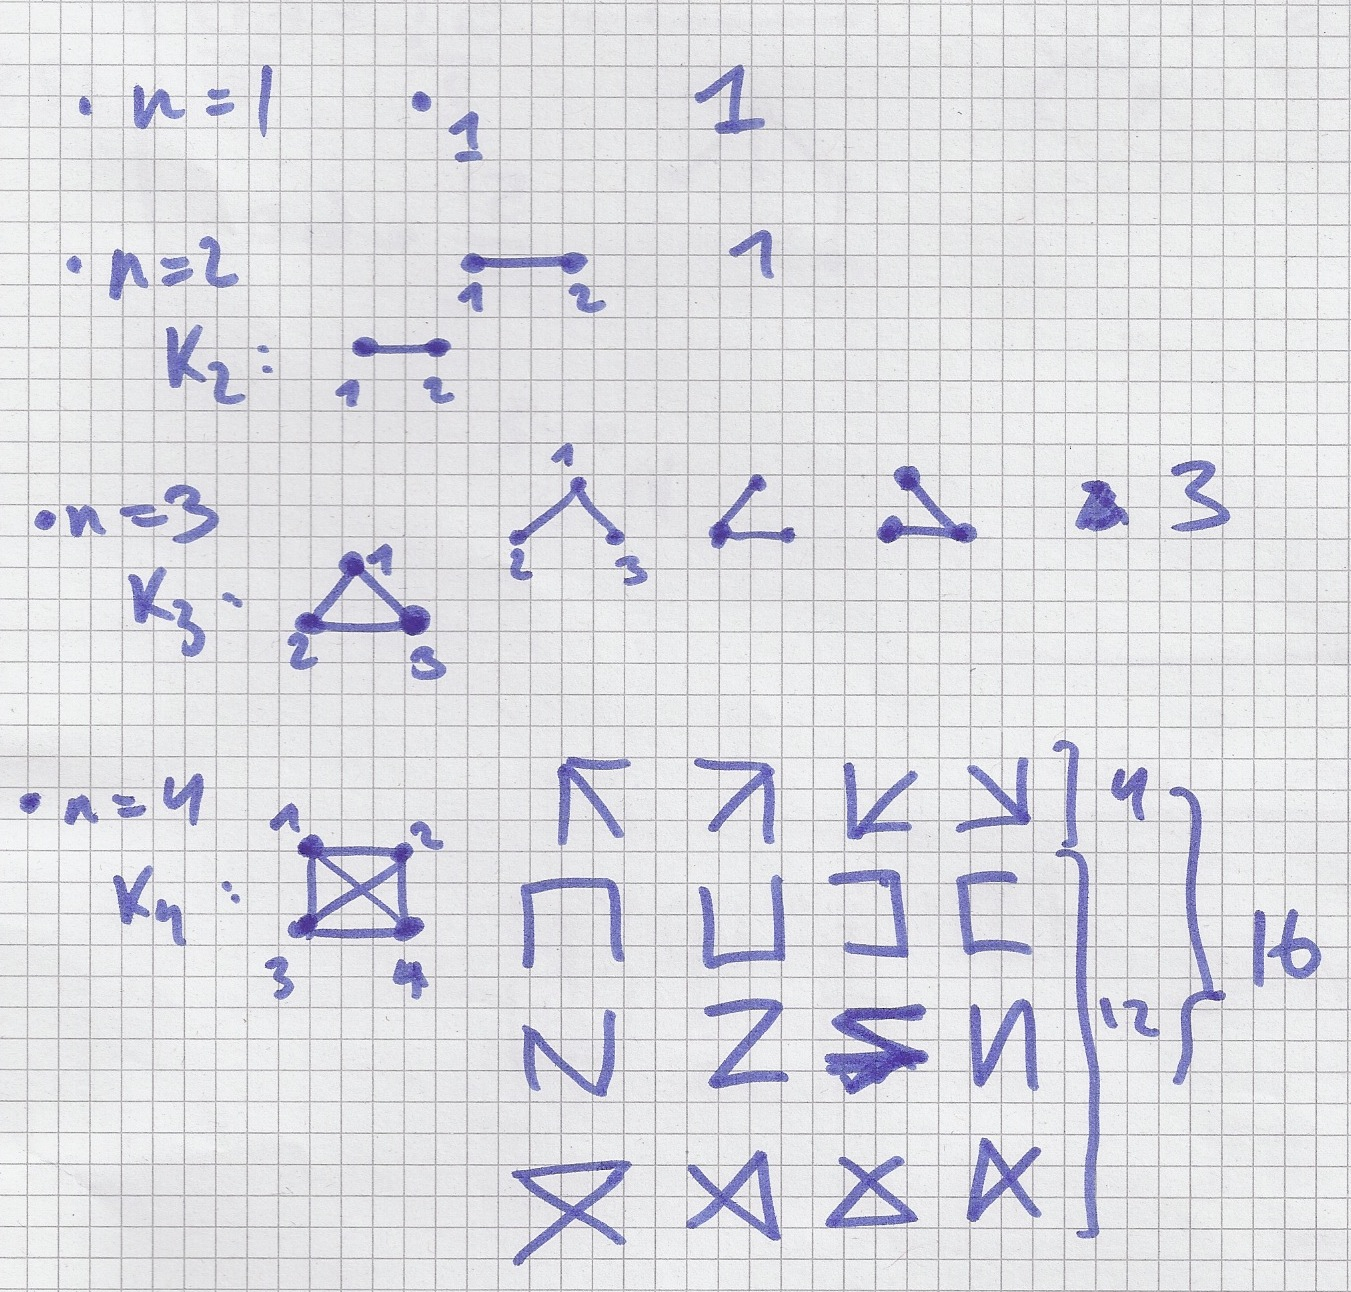
\includegraphics[width=\textwidth]{Bild37} \\
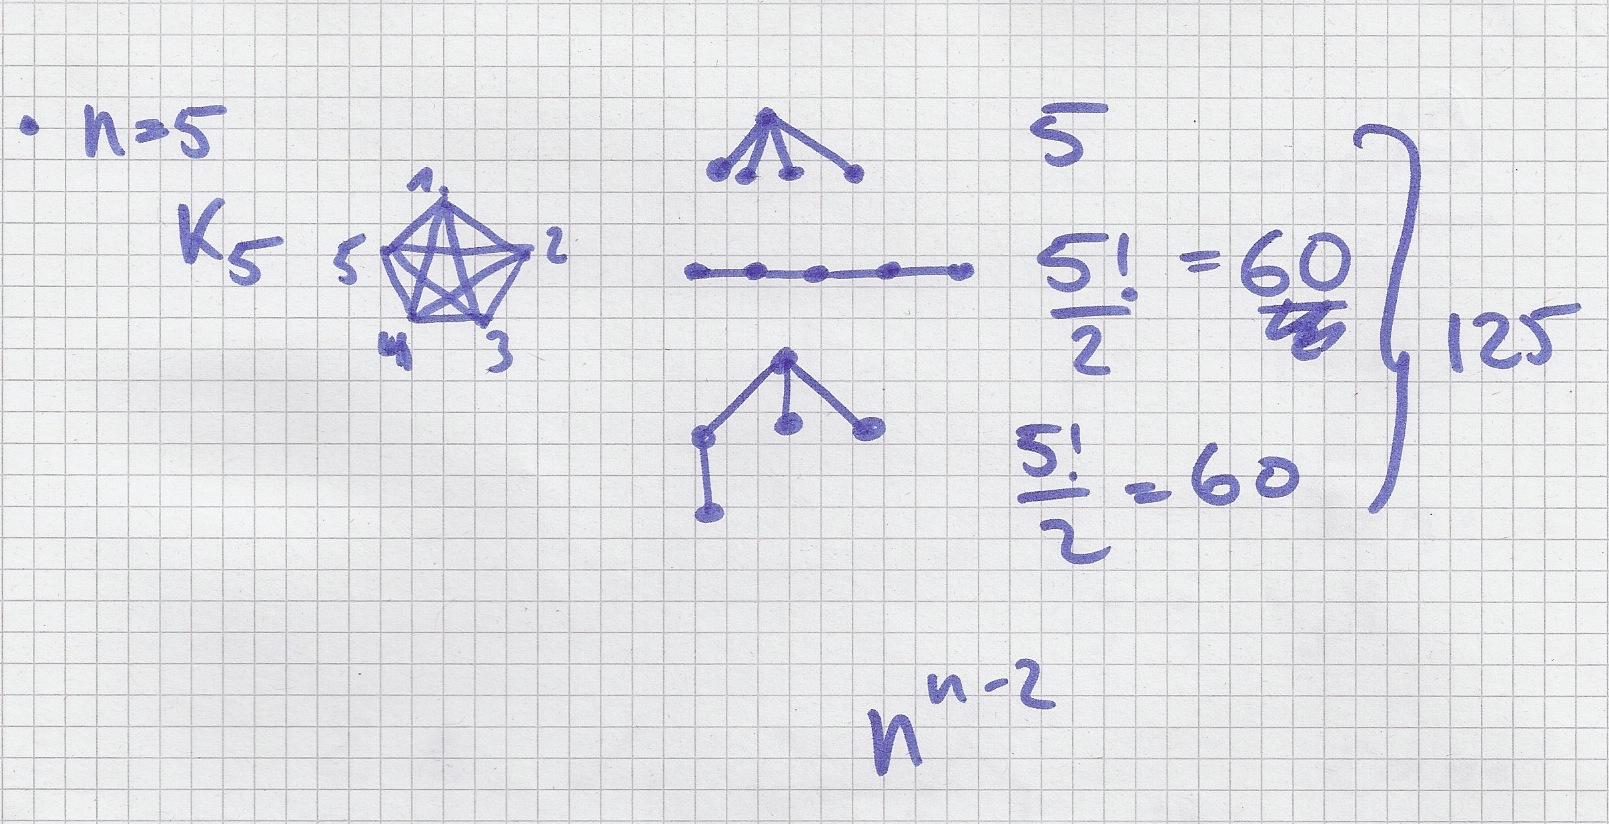
\includegraphics[width=\textwidth]{Bild38}
\begin{def*}[note = isomorph , index = isomorph]
	Zwei Graphen $G=(V,E)$ und $G'=(V',E')$ sind \textbf{isomorph}, $G \cong G'$ falls $\exists f: V \rightarrow V'$ bijektiv so, dass $\forall v,w \in V : (v,w) \in E \iff (f(v),f(w)) \in E'$
\end{def*}
\begin{bsp*}
	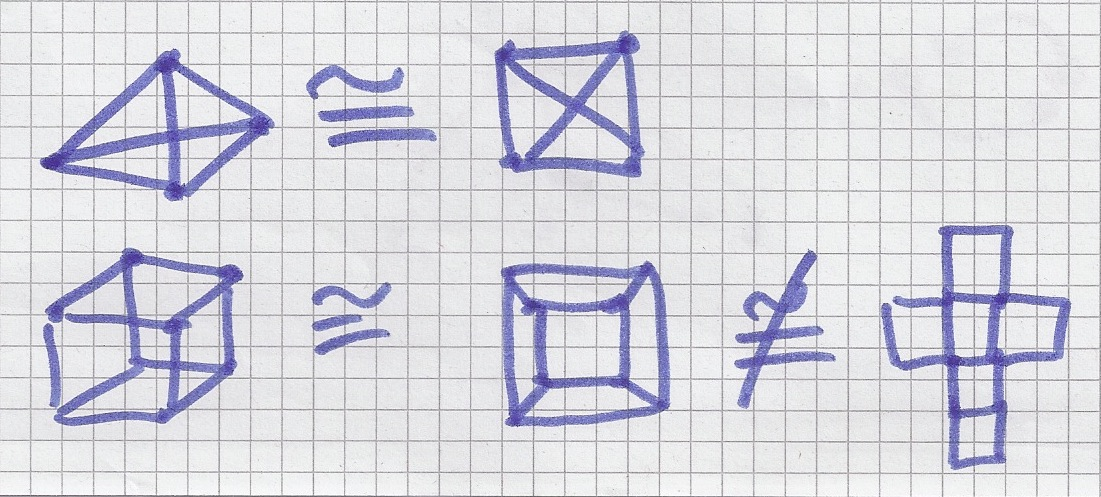
\includegraphics[width=\textwidth]{Bild39}
\end{bsp*}
\begin{satz*}[note = (Cayley)]
	Die Anzahl markierter Bäume mit $n$ Knoten ist $n^{n-2}$
	\begin{bew}
		Wir zählen markierte Bäume mit zwei Zusatzmarkierungen O $\square$, beide beliebig gesetzt.\\
		\begin{bsp*}
			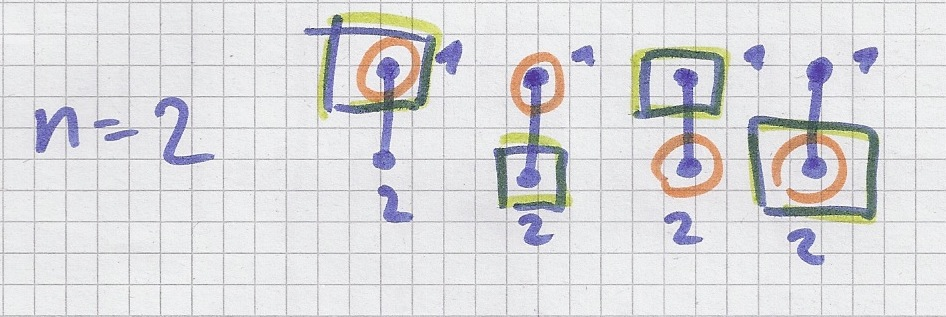
\includegraphics[width=\textwidth]{Bild40}
		\end{bsp*}
		Wir zeigen: von diesen gibt es genau $n^n$.\\
		Bijektion mit $\{f: \{1, \dotsc , n \} \rightarrow \{1, \dotsc , n \} \}$\\
		$\abs{\{\dots\}} = n^n$\\
		$f \mapsto$ markierter Baum mit O $\square$\\
		\[ f = \begin{pmatrix}
			1	&2	&3	&4	&5	&6	&7	&8	&9	&10	\\
			7	&5	&5	&9	&1	&2	&5	&8	&4	&7	
		\end{pmatrix} \]
		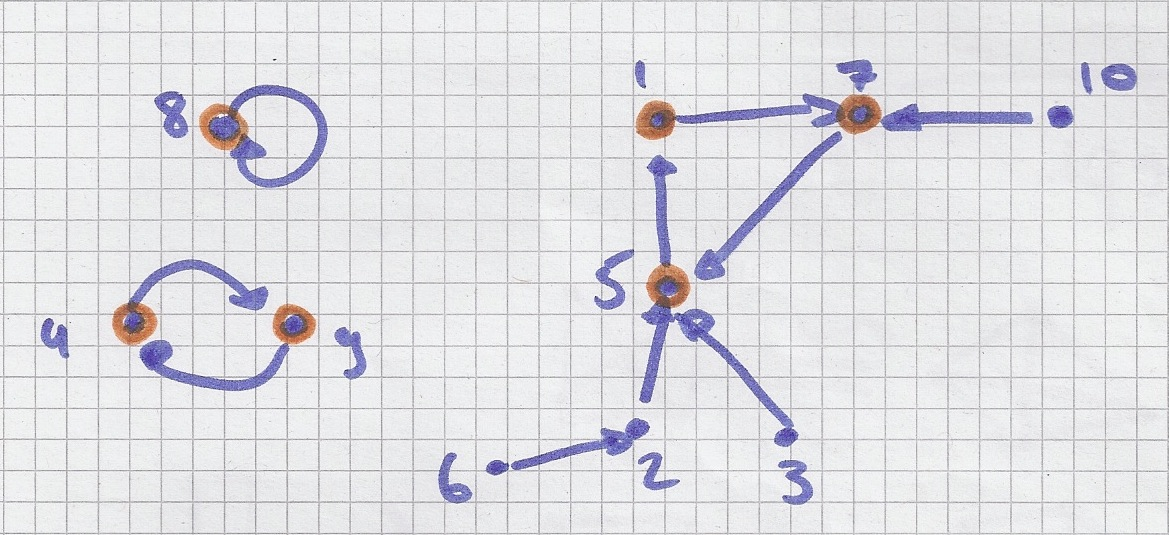
\includegraphics[width=\textwidth]{Bild41} \\
		In jeder Zusammenhangskomponente gibt es einen Zyklus.\\
		Eingeschränkt auf die Knoten M in den Zyklen ist $f$ Bijektion (Permutation)\\
		\[ f|M = \begin{pmatrix}
			1	&4	&5	&7	&8	&9	\\
			7	&9	&1	&5	&8	&4	
		\end{pmatrix} \qquad \text{\enquote{eingeschränkt auf}} \]
		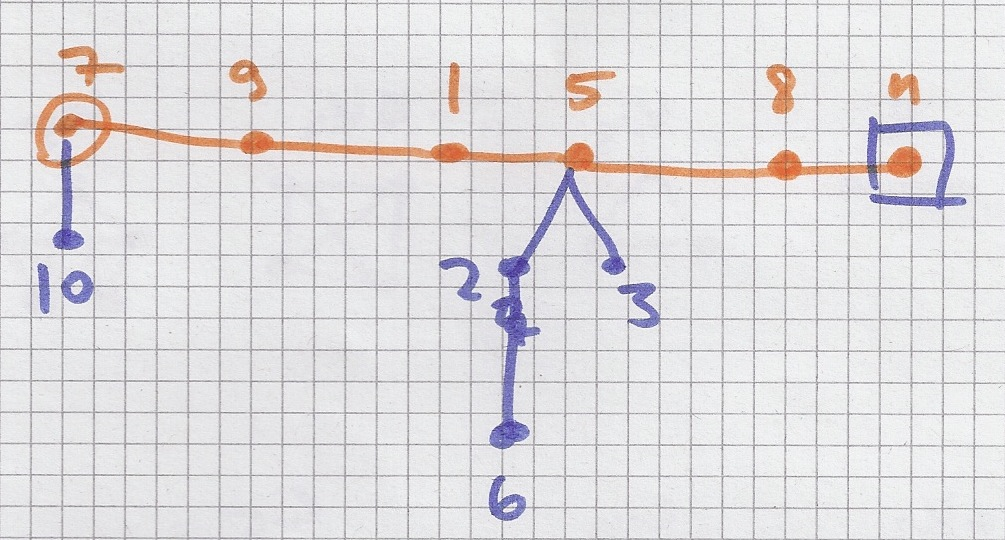
\includegraphics[width=\textwidth]{Bild42}
	\end{bew}
	\begin{bew}[head = Beweis der Umkehrrichtung:]
		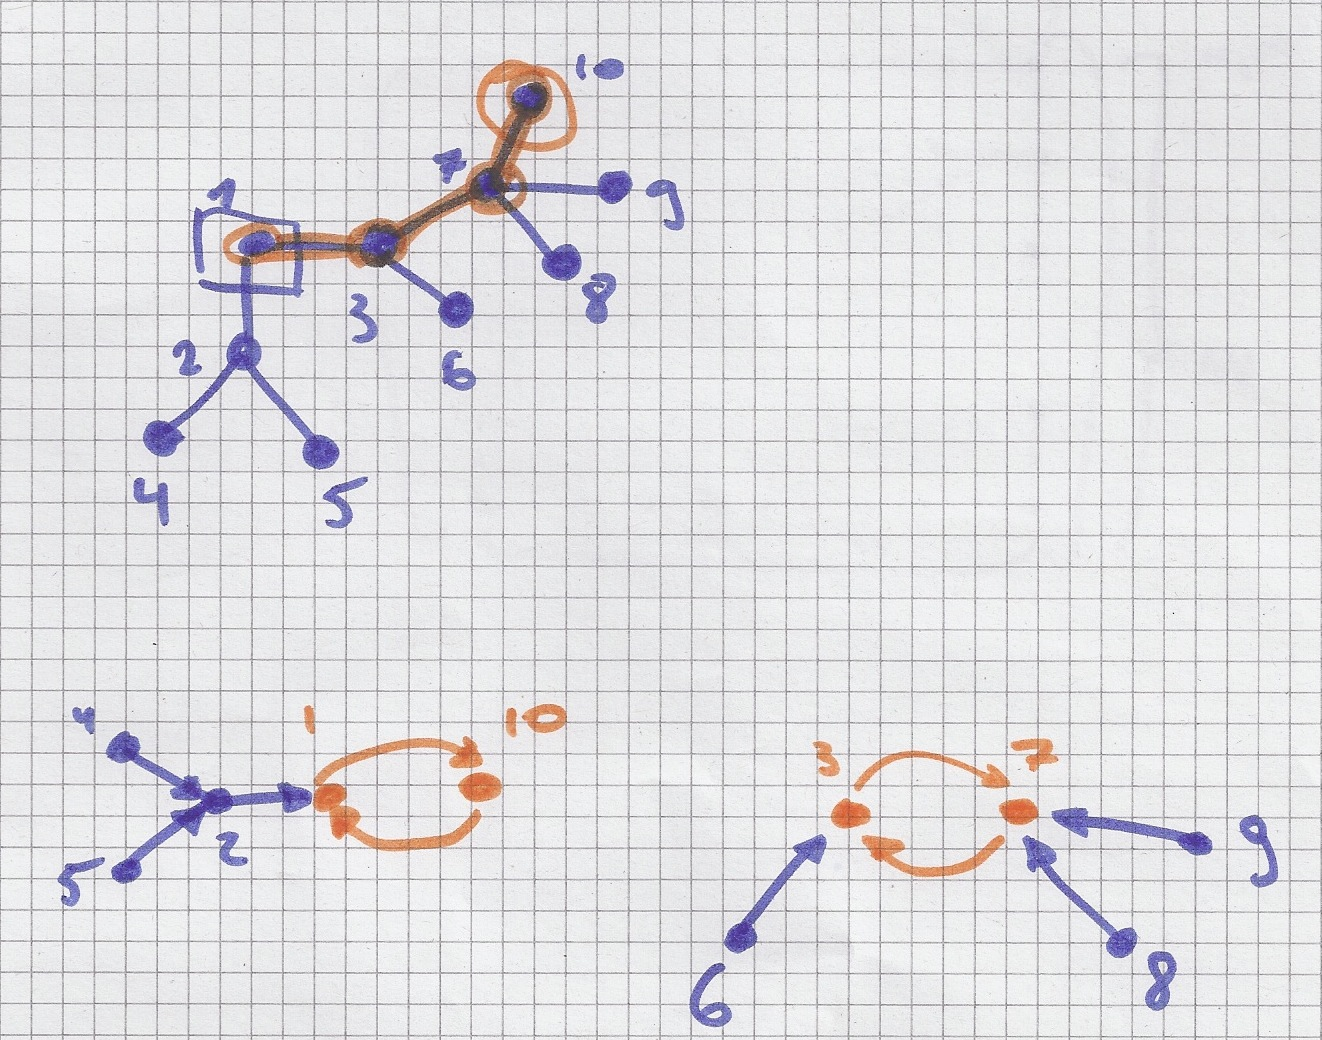
\includegraphics[width=\textwidth]{Bild43}
		\begin{gather*}
			f|M = \begin{pmatrix}
				1	&3	&7	&10	\\
				10	&7	&3	&1	
			\end{pmatrix}\\
			f = \begin{pmatrix}
				1	&2	&3	&4	&5	&6	&7	&8	&9	&10	\\
				10	&1	&7	&2	&2	&3	&3	&7	&7	&1	
			\end{pmatrix}\\
			\blacksquare
		\end{gather*}
	\end{bew}
\end{satz*}
\todo{Too long}

\section{Einige spezielle Graphen}
$K_n$: Vollständiger Graph nit $n$ Knoten (Clique)\\
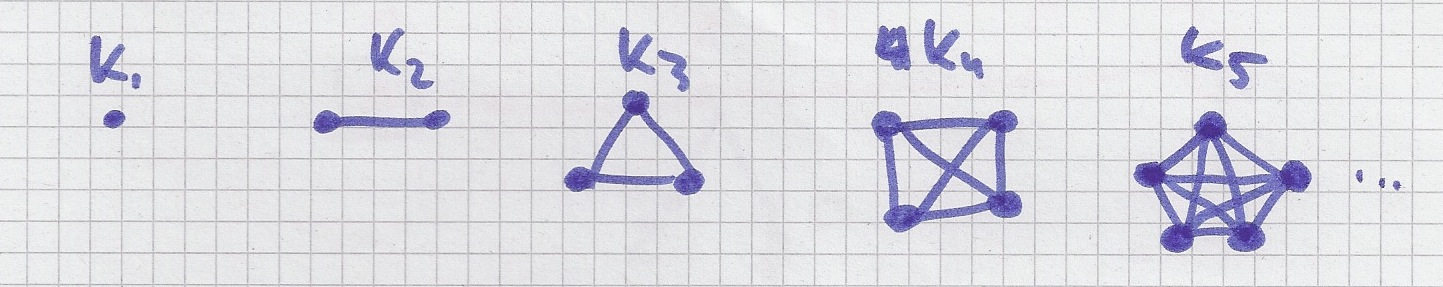
\includegraphics[width=\textwidth]{Bild44} \\
$C_n$: Kreis der Länge $n \:(n\geq 3)$\\
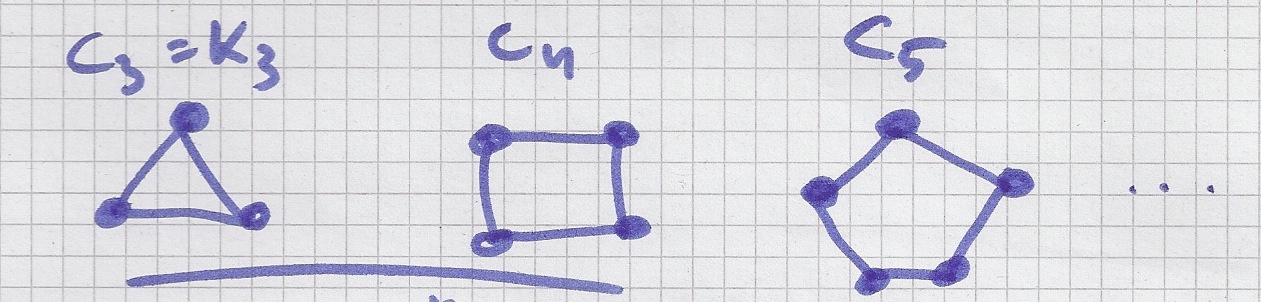
\includegraphics[width=\textwidth]{Bild45} \\
$M_{m,n}$\\
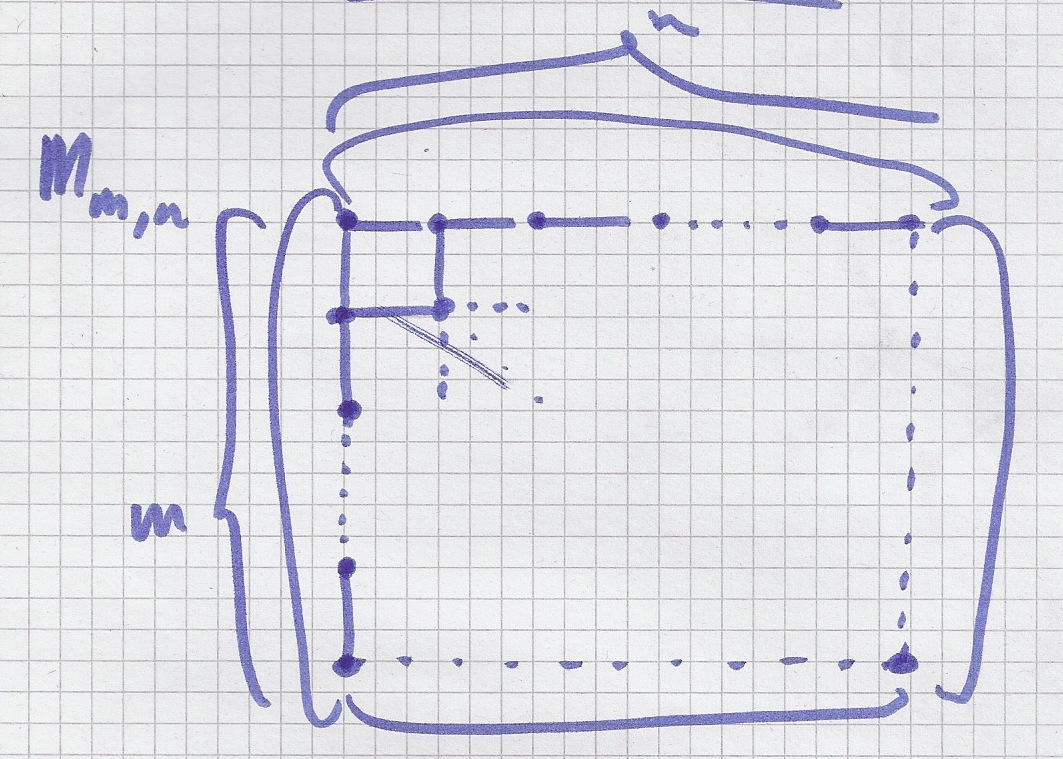
\includegraphics[width=\textwidth]{Bild46} \\
$V = \{ (i,j) : i = 1, \dotsc , m ; j = 1, \dotsc , n \}$\\
$\{(i,j),(i',j')\} \in E \iff \abs{i-i'} + \abs{j-j'} = 1$\\
zyklisch\\
$K_{m,n}$: Vollständiger bipartiter Graph (zwei-färbbar)\\
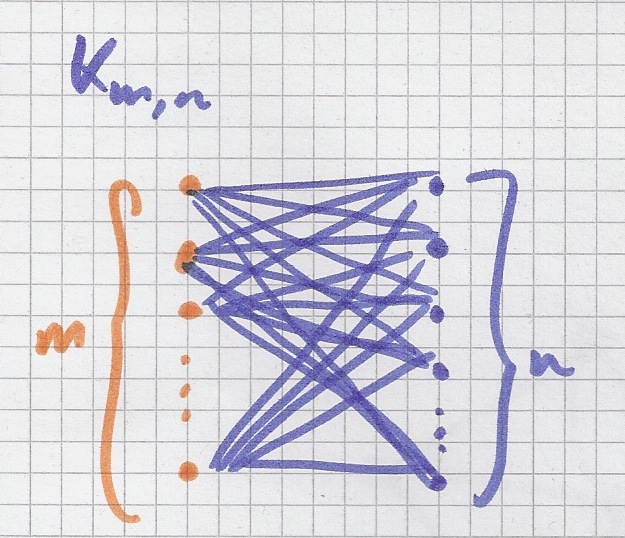
\includegraphics{Bild47} \\
$Q_d$: $d$-dimensionaler Hyperkubus \\
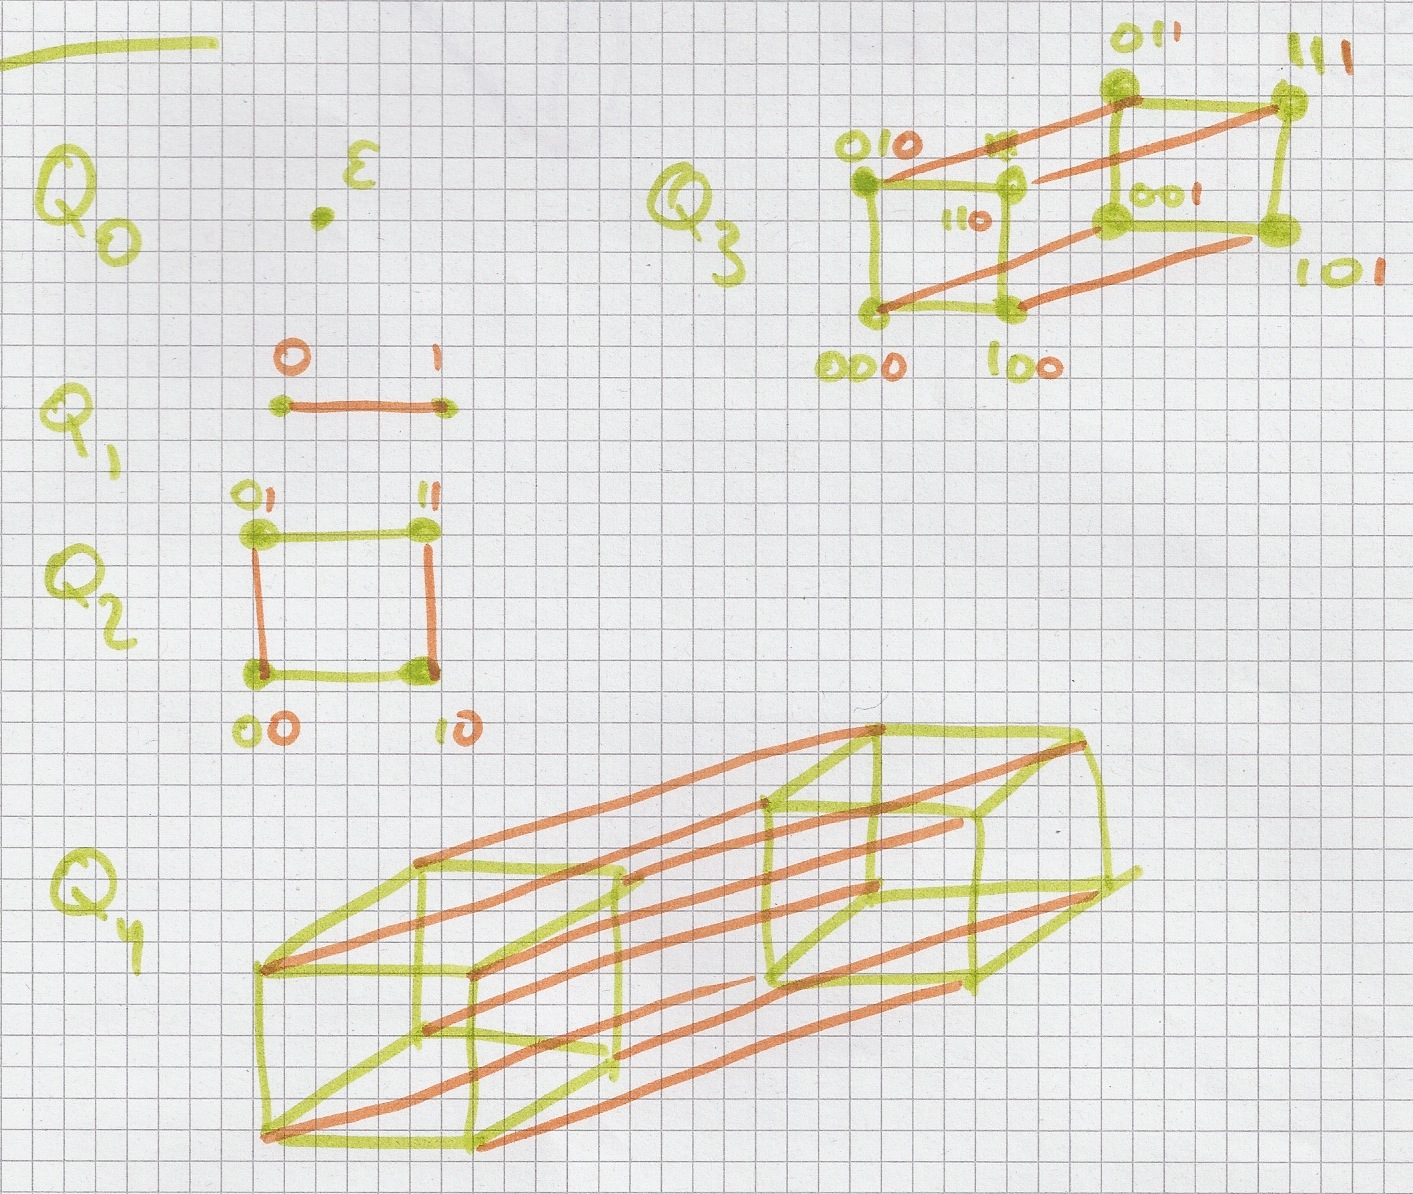
\includegraphics[width=\textwidth]{Bild48} \\
$V = \{ 0 , 1 \}^d$\\
$\{ u , v \} \in E :\iff d_H( u , v ) = 1$\\
$d_H$ ''Hamming-Distanz'': Anzahl differenzierende Bit-Positionen\\
\begin{bsp*}
	\[ d_H( 0110110 , 1011010 ) = 4 \]
\end{bsp*}
\begin{gather*}
	\abs{V} = 2^d \\
	\abs{E} = \frac{\sum_{v \in E} \overbrace{\deg(v)}^{=d}}{2} = \frac{2^d \cdot d}{2} = 2^{d-1} \cdot d
\end{gather*}
\section{Eulertouren und Hamiltonkreise}
\subsubsection{Eulertouren}
Euler (1736): Königsberger Brückenproblem: \\
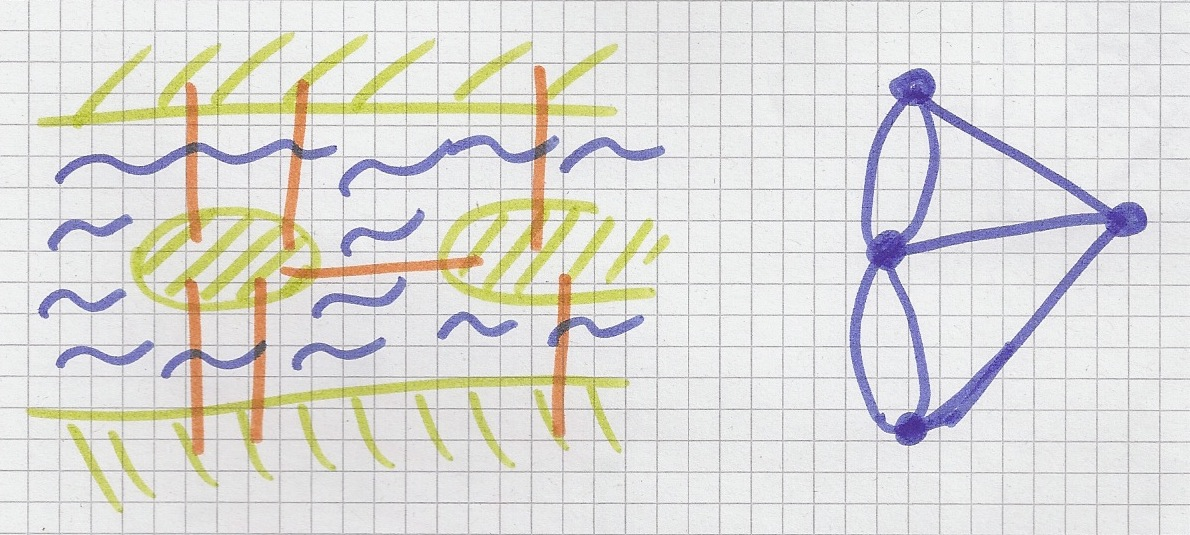
\includegraphics[width=\textwidth]{Bild49} \\
Gibt es einen Weg, der jede Brücke genau einmal benützt? \\
\begin{def*}[note = Eulertour (ET) , index = Eulertour]
	\text{Geschlossener} (Anfang = Ende) Kantenzug, der \textbf{jede Kante} genau einmal enthält.
\end{def*}
Gibt es Eulertour im gegebenen Graphen? Nein. \\
\begin{satz*}[note = (Euler)]
	Ein zusammenhängender Graph (oder Multi-Graph) hat \textbf{genau dann} eine Eulertour, wenn alle Knotengrade gerade sind.\\
	\begin{bew}
		Bedingung notwendig: Jeder Knoten wird gleich oft erreicht und verlassen. \\
		Bedingung hinreichend: Konstruktiv: Zufälliger Knoten $\rightarrow v_1$, jeweils zufällige unbenützte Kante $\rightarrow\rightarrow\rightarrow v_1$. Falls es noch unbenutzte Kanten gibt, dann auch solche, die an $W_1$ grenzen. Analog $W_2$. $\rightarrow W$ geschlossen. Prozess iterieren. Muss abbrechen $(\abs{E} < \infty) \rightarrow$ Eulertour. $\blacksquare$
	\end{bew}
	Wir haben zusätzlich bewiesen: Eine Eulertour kann in linearer Zeit $\sim \abs{E}$ gefunden werden.
\end{satz*}
\begin{bsp*}
	$K_n$ hat ET $\iff$ $n$ ist ungerade. \\
	$Q_d$ hat ET $\iff$ $d$ ist gerade. \\
	Baum $B$ hat keine ET (ausser $\cdot$ )
\end{bsp*}

\subsubsection{Hamiltonkreise}
\begin{def*}[note = Hamiltonkreis (HK) , index = Hamiltonkreis]
	\textbf{Kreis}, der jeden Knoten genau einmal besucht. Ein Graph, der einen HK hat, heisst \text{hamiltonisch}.
\end{def*}
\begin{bsp*}
	hamiltonisch:\\
	$C_k$ \\
	Rad \\
	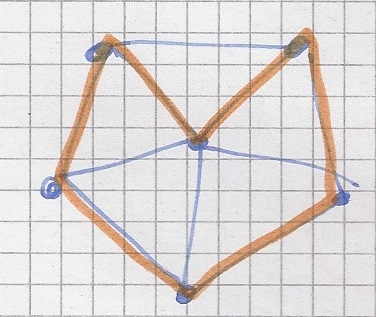
\includegraphics{Bild50} \\
	nicht hamiltonisch: \\
	Stern \\
	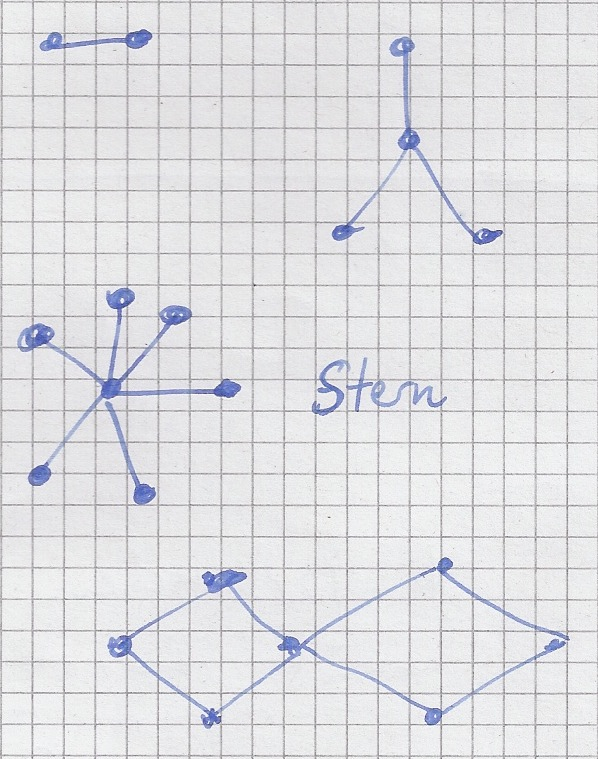
\includegraphics{Bild51} \\
	Bäume
\end{bsp*}
Wann ist $M_{m,n}$ hamiltonisch?\\
\begin{tabular}{lll}
	$M_{1,2}$:	&nicht	&hamiltonisch	\\
	$M_{2,2}$:	&		&hamilotnisch	\\
	$M_{2,3}$:	&		&hamiltonisch	\\
	$M_{3,3}$:	&nicht	&hamiltonisch, da nicht gleich viele gelbe und grüne
\end{tabular}\\
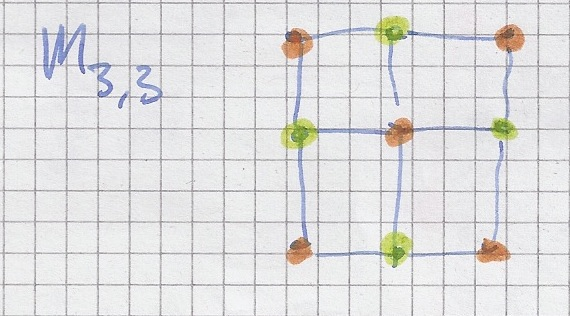
\includegraphics{Bild52} \\
Also: $M_1,n$ nicht hamiltonisch. \\
$m,n \geq 2 : M_{m,n}$ hamiltonisch $\iff m \cdot n = \abs{V}$ gerade \\
\begin{bew}
	$m$ gerade\\
	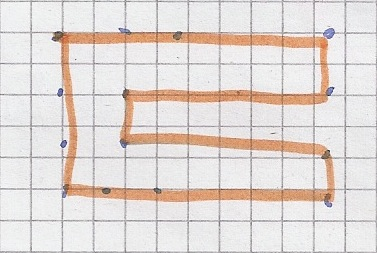
\includegraphics{Bild53}
\end{bew}
Wann ist $Q_d$ hamiltonisch?\\
\begin{tabular}{lll}
	$d=0$:	&nicht	&hamiltonisch	\\
	$d=1$:	&nicht	&hamiltonisch	\\
	$d=2$:	&		&hamiltonisch	\\
	$d=3$:	&		&hamiltonisch	\\
	$d=4$:	&		&hamiltonisch	
\end{tabular}\\
$Q_d$ist hamiltonisch für alle $d \geq 2$.\\
\begin{bew}
	BILD \\
	Induktion über $d$ \\
	Verankerung: $d=2$. \\
	Induktionsschritt: $d \rightarrow d + 1$\\
	IV: $Q_d$ hat HK C. \\
	$C$ und $C'$ enthalten alle Knoten.\\
	Entferne Kanten $(a0,b0)$ und $(a1,b1)$ und fügen $(a0,a1)$ und $(b0,b1)$ ein. $\blacksquare$
\end{bew}
Entscheiden ob ein Graph hamiltonisch ist NP-vollständig. \\
\begin{tabular}{lcl}
	Euler		&$\hat{=}$	&Tautologieproblem KNF	\\
	Hamilton	&$\hat{=}$	&Erfüllbarkeitsproblem DNF	
\end{tabular}\\
\begin{satz*}
	$G=(V,E)$ mit $\deg(v) \geq \frac{\abs{V}}{2}, \abs{V} \geq 4$ für alle $v \implies G$ hamiltonisch. \\
	\begin{bew}
		Indirekt: Gegenbsp. mit max. $\abs{E}$ (für best. $\abs{V}$) \\
		Es gibt $\{ u,v \} \notin E$. ($G$ vollständig $\implies G$ hamiltonisch) \\
		$G' = (V,E \cup \{\{ u,v \}\})$ hat HK (Maximalität von $\abs{E}$) \\
		HK muss $\{ u,v \}$ enthalten (sonst hätte $G$ einen HK) \\
		$\abs{V} = n$ \\
		BILD \\
	\end{bew}
\end{satz*}
	
\section{Planare Graphen}
[Abbot: Flatland]\\
BILD\\
\begin{def*}[note = planar , index = planar]
	$G=(V,E)$ \textbf{planar}, wenn er so gezeichnet werden kann (in die Ebene eingebettet), dass sich keine Kanten überkreuzen (Die Kanten müssen keine Geradestücke sein.
\end{def*}
\begin{satz*}[note = Eulersche Polyederformel , index = Eulersche Polyederformel]
	Sei $G=(V,E)$ zusammenhängender Graph, planar, die Ebene in $f$ Gebiete unterteilt. Dann $\abs{V} + f - \abs{E} = 2$.
	\begin{bew}
		Solange $G$ Kreise enthält, entferne Kanten: $\abs{V}$ unverändert, $\abs{E}: -1$, $f: -1$. Für Bäume stimmt die Formel: $\abs{V} = \abs{E} + 1, f = 1$
	\end{bew}
	\begin{korr*}
		$G=(V,E)$ planar, $\abs{V} \geq 3$. Dann $\abs{E} \leq 3 \abs{V} - 6$\\
		\begin{bew}
			\begin{gather*}
				\abs{V} + f - \abs{E} = 2 \\
				3f \leq 2 \abs{E} \\
				f \leq \frac{2}{3} \abs{E} \\
				\abs{V} + f - \abs{E} = 2 \leq \abs{V} + \frac{2}{3} \abs{E} - \abs{E} = \abs{V} - \frac{\abs{E}}{3} \\
				\abs{E} \leq 3 \abs{V} - 2
			\end{gather*}
		\end{bew}
	\end{korr*}
	\begin{gather*}
		\abs{E} < 3 \abs{V} \\
		\sum_{v \in V} \deg v = 2 \abs{E} < 6 \abs{V} \\
		\frac{\sum_{v \in V} \deg v}{\abs{V}} < 6
	\end{gather*}
\end{satz*}
\todo{Too long}

\begin{gather*}
	K_5: \abs{E} = 10 , \abs{V} = 5 \\
	10 \leq 3 \cdot 5 - 6 = 9 \quad \lightning \\
	\implies K_5 \text{ nicht planar}\\
	\\
	K_{3,3}: \abs{V} = 6 , \abs{E} = 9 \\
	9 \leq 3 \cdot 6 - 6 = 12 ?
\end{gather*}
\begin{korr*}
	$G=(V,E)$ planar und bipartit(Dreiecksfrei), $\abs{V} \geq 3$. Dann $\abs{E} \leq 2 \abs{V} - 4$\\
	\begin{bew}
		\begin{gather*}
				4f \leq 2 \abs{E} \\
				f \leq \frac{\abs{E}}{2} \\
				\abs{V} + f - \abs{E} = 2 \leq \abs{V} + \frac{\abs{E}}{2} - \abs{E} \\
				\abs{E} \leq 2 \abs{V} - 4
		\end{gather*}
	\end{bew}
	\[ \implies \overline{\deg(v)} < 4 \]
\end{korr*}

Nicht planar sind:
\begin{itemize}
	\item $K_5 , K_{3,3}$
	\item $K_6 , K_{3,4} , K_{4,4} , \dotsc$
	\item Graphen, die $K_5$ oder $K_{3,3}$ als Teilgraphen enthalten.
	\item Unterteilungen des $K_5$ oder des $K_{3,3}$ $(*)$
	\item Graphen, die $(*)$ als Teilgraphen enthalten.
\end{itemize}
\begin{satz*}[note = (Kuratowski)]
	Die Liste ist vollständig.
\end{satz*}

\subsection{Färbung von Graphen}
\begin{def*}[note = Knotenfärbung , index = Knotenfärbung]
	\textbf{(Knoten-)Färbung} von $G=(V,E)$ mit $k$ Farben: $c: V \rightarrow \{ 1, 2, \dotsc , k \}$ so, dass $(u,v) \in E \implies c(u) \neq c(v)$.
\end{def*}
\begin{def*}[note = chromatische Zahl , index = chromatische Zahl]
	\textbf{chronatische Zahl} $X(G)$: min. Anzahl Farben $k$, sodass eine $k$-Färbung von $G$ existiert.
\end{def*}
\begin{bsp*}
	\begin{gather*}
		X(K_n) = n \\
		X(K_{m,n}) = 2 \\
		X(M_{m,n}) = 2 \quad ( \neq( m = 1 \wedge n = 1 )) \\
		X(C_n) = \begin{cases}
			2	&n \text{ gerade}	\\
			3	&n \text{ ungerade}
		\end{cases} \\
		X(\text{Baum}) = 2 \quad ( \abs{V} \geq 2 )
	\end{gather*}
\end{bsp*}
\begin{satz*}
	$G=(V,E)$ zusammenhängend, $\abs{V} \geq 2$ bipartit ($X(G) = 2$) \gdw es keinen Kreis ungerader Länge enthält.\\
	\begin{bew}
		\enquote{$\Rightarrow$} klar, da $X($ungerader Kreis$) > 2$ und $X($Teilgraph$) \leq X($Graph$)$ \\
		\enquote{$\Leftarrow$} Spannbaum von $G$. Querverbindungen:
		\begin{itemize}
			\item zwischen Etagen gleicher Parität $\implies$ ungerader Kreis $\implies$ existieren nicht.
			\item ungleicher Parität: kein Problem
		\end{itemize}
	\end{bew}
\end{satz*}

Enscheidung, ob \dots
\begin{itemize}
	\item $X(G) = 2$: lineare Zeit
	\item $X(G) = 3$: NP-vollständig
\end{itemize}

\begin{satz*}
	$G=(V,E)$ planar $\implies X(G) \leq 4$
\end{satz*}
Analoge, \enquote{historisches} Problem: Wie viele Farben sind nötig, um eine Landkarte so einzufärben, dass angrenzende Länder verschiedene Farben haben? (Länder zusammenhängend) $\rightarrow$ Färben planarer Graphen

\begin{description}
	\item[3?] $K_4$ planar
	\item[4?] $K_5$ nicht planar $\implies$ 4-Färbbarkeit möglich.
\end{description}

\begin{satz*}
	$G$ planar $\implies X(G) \leq 6$\\
	\begin{bew}
		\begin{gather*}
			G \text{ planar } \implies \abs{E} \leq 3 \abs{V} - 6 \\
			\sum_{v \in V} \deg(v) = 2 \abs{E} \leq 6\abs{V} - 6 < 6\abs{V} \\
			\frac{1}{\abs{V}} \sum_{v \in V} \deg(v) < 6 \\
			\exists v \in V : \deg(v) < 6
		\end{gather*}
		Induktion über $\abs{V} = n$ \\
		IV: $n \leq 6$ \\
		$n \rightarrow n+1$
	\end{bew}
\end{satz*}

\chapter{Zahlentheorie}
\[ \N , \Z \]
\begin{tabular}{ l c l }
	bisher				&				&ab jetzt					\\ \hline
	Allgemeinheit			&$\leftrightarrow$	&Struktur					\\
	(Mengen, Graphen)		&				&(Zahlen, Graphen, Körper)		\\ \hline
	neu (Euler)				&				&alt (Euklid)				\\ \hline
	(Mathematische			&$\leftrightarrow$	&(Informatikrelevante)			\\
	Informatik				&				&Mathematik				\\ \hline
	sehr viele Anwendungen	&$\leftrightarrow$	&Sehr spezielle, überrraschende	\\
	(Richtige Sprache)		&				&Anwendungen (Kommunikation:	\\
						&				&Kryptographie, Codierung )		
\end{tabular} \\
BILD \\
historisch: populär, einfach(formulierbare) ungelöste Probleme
\begin{itemize}
	\item Goldbach-Vermutung
	\item Gibt es $\infty$ viele Primzahlzwillinge?
	\item Fermat: $x^n + y^n = z^n \quad (n \geq 3 , x, y, z \in \N_{> 0} )$
	\item $x^n - y^n = 1 \quad (m, n \geq 2 , x, y \in \N_{> 0} )$\\
		$3^2 - 2^3 = 1$
\end{itemize}
heute: algorithmische Aspekte: Quelle schwieriger Probleme. \\
Vorgehen: nicht axiomatisch: Grundtatsachen als wahr angenommen\\
\begin{bsp*}
	\begin{itemize}
		\item $a \cdot b = 0 \iff a = 0 \vee b = 0$
		\item $a \geq b \iff -a \leq -b$
		\item $(-a) \cdot b \iff -(a \cdot b)$
		\item $a^2 \geq 0 \forall a$
	\end{itemize}
\end{bsp*}
Erstes Ziel: Existenz und Eindeutigkeit der Primzahlfaktoriesierung. \\
Schlüsseltatsache:
\[ p \text{ prim: } p | a \cdot b \implies p | a \vee p | b \]

\section{Teilbarkeit}
\begin{def*}[note = Teilbarkeit , index = Teilbarkeit]
	\begin{gather*}
		a, b \in \Z, a \neq 0 : \\
		a | b :\iff \exists c \in \Z : a \cdot c = b
		\intertext{Falls $c$ existiert, ist es eindeutig und wir schreiben}
		c = \frac{b}{a}
	\end{gather*}
	\begin{bew}
		\begin{gather*}
			b = ac = ac' \\
			\underbrace{a}_{\neq 0}(c - c') = 0 \\
			\implies c - c' = 0 \\
			c = c' \quad \blacksquare
		\end{gather*}
	\end{bew}
\end{def*}

\subsubsection{Regeln}
\begin{itemize}
	\item $|$ transitiv: $a | b \wedge b | c \implies a | c$
	\item $a | b \wedge b |a \implies a = b \vee a = -b$
	\item $a | b \wedge a | c \implies a | (ub + vc) \quad (u,v \in \Z)$
	\item $a | b \vee a | c \implies a | bc$
	\item $a | 1 \iff a = 1 \vee a = -1$\\
		Nur $1$ und $-1$ haben Inverse. Sie heissen \textbf{Einheiten}.
\end{itemize}

Was ist, wenn $d \nmid a$? \\
\begin{bsp*}
	\begin{gather*}
		5 \nmid 13 \\
		\underbrace{13}_{\text{Dividend}} = \underbrace{2}_{\text{Quotient}} \cdot \underbrace{5}_{\text{Divisor}} + \underbrace{3}_{\text{Rest}}
	\end{gather*}
\end{bsp*}
\begin{satz*}[note = Theorem (Euklid)]
	Für alle $a, d \in \Z, d \neq 0$, gibt es eindeutige $q, r \in \Z$ mit $a = qd + r, 0 \leq v < \abs{d}$. Wir schreiben $r \eqqcolon Rd(a)$ Rest. \\
	\begin{bew}
		Existenz
		\begin{gather*}
			d > 0 \\
			qd \leq a < (q+1)d \\
			0 \leq r < dq
		\end{gather*}
		Eindeutigkeit
		\begin{gather*}
			0 \leq r < \abs{d} \\
			0 \leq r' < \abs{d} \\
			a = qd + r = q'd + r \\
			\underbrace{(q-q')}_{\substack{\text{Vielfaches}\\\text{von } d}} d = \underbrace{r'-r}_{\abs{r'-r} < d} \implies r'-r = 0 \\
			r = r' \\
			q = q' \quad \blacksquare
		\end{gather*}
	\end{bew}
\end{satz*}

\section{Ideale, ggT, Euklid-Algorithmus}
35, 55 und 77 min Uhren \\
Welche Zeitspannen lassen sich damit abmessen? \\
35, 55 und 77 Massstäbe \\
Welche Distanzen lassen sich messen?  \\
Es lassen sich genau folgende Distanzen messen:
\[ \{ 35u + 55v + 77w | u, v, w \in \Z \} \eqqcolon (35,55,77) \textbf{ Ideal} \]
Wie sieht diese Menge aus? \\
Welche Zahlen haben die Form $35u + 55v$? \\
$55, 35, 20, 40, 60, 5, 10, 15, \dotsc$ \\
Vermutung: $(35,55) = (5) = \{ 5z | z \in \Z \} = 5\Z$ \\
$= \Z = (1)$

\begin{def*}[note = Ideal , index = Ideal]
	Das von $a_1, \dotsc , a_n$ erzeugte \textbf{Ideal} ist
	\[ ( a_1, \dotsc , a_n ) \coloneqq \{ \sum_{i=1}^n u_i a_i | u_i \in \Z \} \subseteqq \Z \]
\end{def*}
\begin{satz*}
	Für alle $a_i \in \Z, i=1, \dotsc , n$ gibt es $d \in \Z$ mit $(a_1 , \dotsc , a_n) = (d) = d\Z$.
	\begin{bew}
		Der Fall$n=2$\\
		Zu zeigen $(a,b) = d$ für geeignetes $d$. \\
		Sei $d$ das kleinste Element von $(a,b)$, daas $> 0$ ist. \\
		Jetzt $(d) \subseteq (a,b)$
		\begin{gather*}
			d \in (a,b) \\
			d = u_1 a + u_2 b \\
			v \in \Z : v d = ( v u_1) a + (v u_2) b \in (a,b)
		\end{gather*}
		$(d) \supseteq (a,b)$\\
		Sei nun $x \in (a,b)$ Dann \\
		\begin{gather*}
			\underbrace{x}_{u_3 a + u_4 b} = q \underbrace{d}_{u_1 a + u_2 b} + \underbrace{r}_{0 \leq r < d} \quad \text{Euklid} \\
			r = (u_3 - q u_1) a + (u_4 - q u_2)b \in (a,b) \\
			\implies r = 0 \\ 
			\implies x = q d \\
			x \in (d) \\
			\text{Also } (a,b) \subseteq (d)
		\end{gather*}
		$n=3$
		\begin{align*}
			(a,b,c)	&= \{ \underbrace{u_1 a + u_2 b}_{v d} + u_3 c | u_i \in \Z \} \\
					&= \{ v d + u_3 c | v, u_3 \in \Z \} = (e)
		\end{align*}
		Beliebige $n$: Induktion $\blacksquare$
	\end{bew}
\end{satz*}
\begin{def*}[note = ggT , index = ggT]
	$a, b \in \Z , (a,b) \neq (0,0)$\\
	Dann heisst $d$ \textbf{ggT} von $a$ und $b$ falls:
	\begin{itemize}
		\item $d|a$
		\item $d|b$
		\item $c|a \wedge c|b \implies c|d$
	\end{itemize}
	\begin{bem}
		ggT von $4$ und $6$ sind $2$ und $-2$.
	\end{bem}
	Für den positiven schreiben wir $\ggt(a,b)$. \\
	$a \neq 0 : \ggt(a,0) = \abs{a}$
\end{def*}
\begin{satz*}
	\[ (a,b) = (\ggt(a,b)) \]
	\begin{bew}
		\begin{gather*}
			(a,b) = (d) \implies d|a , d|b \\
			c|a \wedge c|b \implies c|\underbrace{(ua+vb)}_{d} \iff c|d \\
			\implies d = \ggt(a,b)
		\end{gather*}
	\end{bew}
	\begin{bem}
		Man schriebt oft $(a,b)$ für $\ggt(a,b)$.
	\end{bem}
\end{satz*}
\begin{korr*}
	$a, b \in \Z, (a,b) \neq (0,0)$ \\
	Dann existieren $u, v \in \Z : ua + vb = \ggt(a,b)$ \\
	$u, v$ können mit dem Erweiterten Euklidischen Algorithmus berechnet werden. \\
	\[ \begin{array}{ | r | c | c | c | c l | }
		\hline
						&	&	&(24)	&(9)	&	\\ \hline
						&a	&24	&1	&0	&	\\ \hline
		24 = q \cdot 9 + r	&b	&9	&0	&1	&	\\ \hline
		a = q \cdot b + r_1	&r_1	&6	&1	&-2	&	\\ \hline
		b = q \cdot r_1 + r_2	&r_2	&3	&-1	&3	&\rightarrow \ggt(24,9) = 3 = \overbrace{(-1)}^u \cdot 24 + \overbrace{3}^v \cdot 9	\\ \hline
						&	&0	&	&	&	\\ \hline
	\end{array} \]
\end{korr*}
\begin{bsp*}
	\begin{gather*}
		\begin{array}{ | c | c | c | }
			\hline
				&(55)	&(35)	\\ \hline
			55	&1	&0	\\ \hline
			35	&0	&1	\\ \hline
			20	&1	&-1	\\ \hline
			15	&-1	&2	\\ \hline
			5	&2	&-3	\\ \hline
			0	&	&	\\ \hline
		\end{array} \\
		5 = 2 \cdot 55 + (-3) \cdot 35 \\
		\begin{array}{ | c | c | c | }
			\hline
				&(77)	&(5)	\\ \hline
			77	&1	&0	\\ \hline
			5	&0	&1	\\ \hline
			2	&1	&-15	\\ \hline
			1	&-2	&31	\\ \hline
		\end{array} \\
		77 = 15 \cdot 5 + 2 \\
		5 = 2 \cdot 2 + 1 \\
		1 = (-2) \cdot 77 + 31 \cdot 5 = (-2) \cdot 77 + 62 \cdot 55 + (-93) \cdot 35 \\
		3 = (-6) \cdot 77 + 186 \cdot 55 + (-279) \cdot 35
	\end{gather*}
\end{bsp*}

\section{Primfaktorzerlegung}
\begin{def*}[note = Prim , index = Prim]
	\[ p \in \N , p > 1 , \text{ prim} \]
	falls die einzigen positiven Teiler von $p$ $1$ und $p$.
\end{def*}
\begin{satz*}
	\begin{gather*}
		a, b \in \Z \\
		p | a \cdot b \implies p | a \vee p | b \quad \blacksquare
	\end{gather*}
	\begin{bew}
		\begin{gather*}
			p |ab , p \nmid a , p \Prim \implies \ggt(p,a) = 1 \\
			\exists u, v : 1 = u p + v a \implies b = \underbrace{u p b}_{p|\cdot} + v \underbrace{a b}_{p|\cdot}
		\end{gather*}
	\end{bew}
\end{satz*}
\begin{satz*}[note = Fundamentalsatz der Arithmetik]
	Jede Zahl $n \in \N , n \geq 1$, \textbf{besitzt} eine \textbf{eindeutige} (bis auf die Reihenfolge der Faktoren) \textbf{Primfaktorzerlegung}.
	\begin{bew}[note = Existenz]
		Indirekt: \\
		Sei $n$ die kleinste Zahl ohne Zerlegung. Dann ist $n$ nicht prim. Also hat $n$ einen Teiler $m , 1 < m < n : n = m k ; m , k < n$. $m, k$ haben Zerlegungen $\implies n$ hat Zerlegung $\lightning$.
	\end{bew}
	\begin{bew}[note = Eindeutigkeit]
		Sei $n$ die kleinste Zahl mit zwei verschiedenen Zerlegungen.
		\begin{gather*}
			n = \underbrace{p_1^{e_1} p_2^{e_2} \dots p_r^{e_r}}_{e_i > 0} = \underbrace{q_1^{f_1} q_2^{f_2} \dots q_s^{f_s}}_{f_i > 0} \\
			p_1 | q_1^{f_1} (q_2^{f_2} \dots q_s^{f_s}) \underset{p \text{ prim}}{\implies} p_1 | q_1 \vee p_1 | q_2^{f_2} \dots q_s^{f_s} \\
			\implies \exists j : p_1 | q_j^{f_j} \implies p_1 | q_j \implies p_1 = q_j \\
		\end{gather*}
		$\frac{n}{p_1}$ hat zwei verschiedene Darstellungen $\lightning \quad \blacksquare$
	\end{bew}
\end{satz*}

\subsubsection{ggT und kgV}
\begin{def*}[note = kgV , index = kgV]
	$a, b > 0$. Dann heisst \\
	$l$ kleinstes gemeinsames Vielfaches von $a, b ; l = \kgv(a,b)$, falls:
	\begin{itemize}
		\item $a|l$
		\item $b|l$
		\item $a|m \wedge b|m \implies l|m$
	\end{itemize}
\end{def*}
Falls $\prod p_i^{e_i} , \prod p_i^{f_i}$
\begin{gather*}
	\ggt(a,b) = \prod p_i^{\min(e_i , f_i)} \\
	\kgv(a,b) = \prod p_i^{\max(e_i , f_i)} \\
	\implies \ggt \cdot \kgv = \prod p_i^{\overbrace{\min(e_i , f_i) + \max(e_i , f_i)}^{e_i + f_i}} = \prod p_i^{e_i} \cdot \prod p_i^{f_i} = a b
\end{gather*}

\subsubsection{Weiteres zu Primzahlen}
\begin{itemize}
	\item Es gibt unendlich viele Primzahlen.
	\item Es gibt beliebig gross Lücken: $[n!+2 , n!+n]$ enthält keine Primzahl, denn $k|n!+k$ für $k \leq n$
	\item Dichte: $\pi(n) = \abs{\{ 1 < k < n | k \text{ prim} \}}$ \\
		$\pi(n) \sim \frac{n}{\ln n}$ zB. ''Jede 230-ste 100-stellige Zahl ist prim''
	\item Primzahltests?
		\begin{itemize}
			\item ''Primes is in P''
			\item Probabilistische Methode \\
				$p$ prim $\implies a^{p-1} \equiv 1 \pmod p$ \\
				$a^{p-1} \not\equiv 1 \pmod p \implies p$ nicht prim
		\end{itemize}
\end{itemize}

\section{Modulare Arithmetik}
\begin{def*}[note = kongruent , index = kongruent]
	\begin{gather*}
		a, b \in \Z , m > 1 \\
		a \equiv n \pmod m :\iff  m | (a-b)
	\end{gather*}
	Äquivalent: $a = b + zm \quad z \in \Z$\\
\end{def*}
Es gilt: $a \equiv b \pmod m \iff R_m(a) = R_m(b)$ \\
\begin{bew}
	\begin{gather*}
		a = q_1 m + R_m(a) \\
		b = q_2 m + R_m(b) \\
		0 \leq R_m(\cdot) < m \\
		\begin{split}
			a \equiv b \pmod m	&\iff m | (a-b) \\
							&\iff m | (\underbrace{R_m(a) - R_m(b)}_{-m< \dots <m}) \\
							&\iff R_m(a) = R_m(b)
		\end{split}
	\end{gather*}
\end{bew}
\begin{gather*}
	a \equiv R_m(a) \pmod m \\
	R_m(a) = R_m(R_m(a))
\end{gather*}
\begin{satz*}
	\begin{gather*}
		R_m(a + b) = R_m(R_m(a) + R_m(b)) \\
		R_m(a \cdot b) = R_m(R_m(a) \cdot R_m(b))
	\end{gather*}
	\begin{bew}
		\[ a + b \equiv_m R_m(a) + R_m(b) \quad \blacksquare \]
	\end{bew}
\end{satz*}
Anwendungen:
\begin{itemize}
	\item Vereinfachen von Rechnungen $R_m(a^x)$
	\item Kontrollieren von Rechnen
	\item Die meisten Zahlen beginnen mit 1, 2 oder 3
\end{itemize}

$\equiv_m$ ist Äquivalenzrelation\\
\begin{bew}
	\begin{gather*}
		a \equiv_m a \quad \checkmark \text{ reflexiv} \\
		a \equiv_m b \iff b \equiv_m a\quad \checkmark \\
		a \equiv_m b \wedge b \equiv_m c \implies a \equiv_m c \\
		m | (a-b) \wedge m | (b-c) \implies m | (a-b) + (b-c) \iff m | (a-c)\quad \checkmark
	\end{gather*}
\end{bew}

Äquivalenzklassen
\begin{gather*}
	\{ [0] , [1] , \dotsc , [m-1] \} \eqqcolon \Z_m \\
	\left. \begin{matrix*}[l]
		[a] + [b] \coloneqq [a+b] \\
		[a] \cdot [b] \coloneqq [a \cdot b]
	\end{matrix*} \right\} \text{ wohldefiniert}\\
	\\
	\Z_5 \\
	\begin{matrix}
		+	&0	&1	&2	&3	&4	\\
		0	&0	&1	&2	&3	&4	\\
		1	&1	&2	&3	&4	&0	\\
		2	&2	&3	&4	&0	&1	\\
		3	&3	&4	&0	&1	&2	\\
		4	&4	&0	&1	&2	&3	
	\end{matrix} \qquad
	\begin{matrix}
		\cdot	&0	&1	&2	&3	&4	\\
		0	&0	&0	&0	&0	&0	\\
		1	&0	&1	&2	&3	&4	\\
		2	&0	&2	&4	&1	&3	\\
		3	&0	&3	&1	&4	&2	\\
		4	&0	&4	&3	&2	&1	
	\end{matrix}\\
	\Z_6 \\
	\begin{matrix}
		+	&0	&1	&2	&3	&4	&5	\\
		0	&0	&1	&2	&3	&4	&5	\\
		1	&1	&2	&3	&4	&5	&1	\\
		2	&2	&3	&4	&5	&0	&2	\\
		3	&3	&4	&5	&0	&1	&3	\\
		4	&4	&5	&0	&1	&2	&4	\\
		5	&5	&0	&1	&2	&3	&4	\\
	\end{matrix} \qquad
	\begin{matrix}
		\cdot	&0	&1	&2	&3	&4	&5	\\
		0	&0	&0	&0	&0	&0	&0	\\
		1	&0	&1	&2	&3	&4	&5	\\
		2	&0	&2	&4	&0	&2	&4	\\
		3	&0	&3	&0	&3	&0	&3	\\
		4	&0	&4	&2	&0	&4	&2	\\
		5	&0	&5	&4	&3	&2	&1	\\
	\end{matrix} \\
\end{gather*}
\begin{tabular}{ r | c | c | c | c }
				&Kommutativ	&Assoziativ	&Neutralelement		&Inverse			\\ \hline
	Addition		&$\checkmark$	&$\checkmark$	&$\checkmark (0)$	&$\checkmark (-a)$	\\
	Multiplikation	&$\checkmark$	&$\checkmark$	&$\checkmark (1)$	&???				
\end{tabular}

\subsubsection{Multiplikative Inverse?}
\begin{gather*}
	a \in \Z_m \\
	[a] \cdot [x] = [1] \\
	a \cdot x \equiv 1 \pmod m \\
	\intertext{Hat}
	\underbrace{a \cdot x}_{d \mid} = \underbrace{1 + l \cdot m}_{d \nmid} \quad ( k \in \Z )
	\intertext{immer eine Lösung?}
\end{gather*}
\uline{Nein}, falls $a = 0$ \\
\uline{Nein}, falls $\ggt(a,m) = d > 1$ \\
\uline{Ja}, falls $\ggt(a,m) = 1$ \\
\begin{gather*}
	\exists u , v : u \cdot a + v \cdot m = 1 \\
	u \cdot a \equiv 1 \pmod m \\
	u \equiv a^{-1} \pmod m
\end{gather*}
Inverse können mit erweitertem Euklid berechnet werden.
\begin{gather*}
	\Z_5^* = \Z_5 \setminus \{ 0 \} = \{ 1 , 2 , 3 , 4 \} \\
	\Z_6^* = \{ 1 , 5 \} \\
	\Z_m^* = \{ a \in \Z_m \mid \ggt(a,m) = 1 \}
\end{gather*}
Ziel: Verständnis von Public-Key Kryptosysteme
$( \Z_m , + )$: Einfache Struktur, alle Elemente haben Inverse. Unbrauchbar für Kryptographie. \\
$( \Z_m^* , \cdot )$: geeignet. \\
Verständnis von $\Z_m^*$:
\begin{itemize}
	\item Chinesische Restsatz
	\item Gruppe
\end{itemize}

\subsubsection{Der chinesischer Restsatz}
\begin{gather*}
	\left. \begin{matrix*}[l]
		x \equiv 2 \pmod 3 \\
		x \equiv 3 \pmod 5
	\end{matrix*} \right\} \iff x \equiv 8 \pmod 15 \\
	\intertext{aber:}
	\left. \begin{matrix*}[l]
		x \equiv 1 \pmod 6 \\
		x \equiv 2 \pmod 8
	\end{matrix*} \right\} \iff \text{ keine Lösung}
\end{gather*}
\begin{satz*}[note = Chinesischer Restsatz (CRS):]
	$m_i , i = 1 , \dotsc , r$, paarweise teilerfremd: \\
	\begin{gather*}
		\ggt(m_i , m_j) = 1 \text{ für } i \neq j \\
		a_i \in \Z \\
		\intertext{Dann ist}
		\left. \begin{matrix*}[l]
			x \equiv a_1 \pmod {m_1} \\
			x \equiv a_2 \pmod {m_2} \\
			\vdots \\
			x \equiv a_r \pmod {m_r}
		\end{matrix*} \right\} *
		\intertext{äquivalent zu einer Kongruenz}
		x \equiv a \pmod M \\
		M = \prod_{i=1}^r m_i
	\end{gather*}
	Mit anderen Worten, $*$ hat genau eine Lösung $a$ in $\{0 , \dotsc , M-1 \}$, und $a$ kann effizient berechnet werden.
	\begin{bew}[head = Beweisidee:]
		\begin{gather*}
			x_1 \equiv  1 \pmod 3 \\
			x_1 \equiv 0 \pmod 5 \\
			x_2 \equiv 0 \pmod 3 \\
			x_2 \equiv 1 \pmod 5 \\
			\text{Dann: } x = 2 x_1 + 3 x_2 \\
			x_1 = \underbrace{5 ( \cdot 5^{-1} \pmod 3 )}_{\substack{\equiv 1 \pmod 3 \\ = -1}} = -5 \\
			x_2 = 3 \cdot ( \underbrace{3^{-1} \pmod 5}_{2} ) = 6
			\intertext{Existenz}
			M = \prod m_i \\
			M_i \coloneqq \frac{M}{m_i} = m_1 m_2 \dotsm m_{i-1} m_{i+1} \dotsm m_r \\
			\text{Dann } \ggt(M_i , m_i) = 1 \quad (m_i \text{ teilerfremd}) \\
			\text{Also gibt es $N_i$ mit} \\
			M_i N_i \equiv 1 \pmod m_1 \quad ( N_i \equiv M_i^{-1} \pmod {m_i} ) \\
			M_i N_i \equiv 0 \pmod {m_j} \quad j \neq i \\
			\text{Lösung: } R_M \left( \sum_{i=1}^r a_i M_i N_i \right) \\
			a_1 M_1 N_1 + \dots + a_r M_r N_r \equiv a_1 \pmod {m_1} \\
			\intertext{Eindeutigkeit}
			\text{Lösungen } x , x' \in * \\
			m_i \mid (x - x') \\
			\implies \prod m_i \mid (x - x') \implies x \equiv x' \pmod M \quad \blacksquare
		\end{gather*}
	\end{bew}
\end{satz*}
Konsequenz: Spezialfall $m = p q ; p , q$ prim, $p \neq q$ \\
\begin{gather*}
	\left. \begin{matrix*}[l]
		x \equiv a_1 \pmod p \\
		x \equiv a_2 \pmod q
	\end{matrix*} \right\} \iff x \equiv a \pmod {p q} \\
	\Z_m = \Z_p \times \Z_q \\
	a \in \Z_m \leftrightarrow \begin{pmatrix} a_1 \\ a_2 \end{pmatrix} \begin{matrix} \in \Z_p \\ \in \Z_q \end{matrix} \\
	\begin{split}
		''\rightarrow'' :	&a_1 = R_p(a) \equiv a \\
					&a_2 = R_q(a) \equiv a
	\end{split} \\
	''\leftarrow'' : \text{ CRS} \\
	a = R_m( a_1 \underbrace{M_1 N_1}_{q \cdot q^{-1} \pmod p} + a_2 \underbrace{M_2 N_2}_{p \cdot p^{-1} \pmod q} )
\end{gather*}

Verträglichkeit der Operationen:
\begin{gather*}
	a \leftrightarrow \begin{pmatrix} a_1 \\ a_2 \end{pmatrix} \\
	b \leftrightarrow \begin{pmatrix} b_1 \\ b_2 \end{pmatrix} \\
	a + b \leftrightarrow \begin{pmatrix} a_1 + b_1 \\ a_2 + b_2 \end{pmatrix} \\
	a \cdot b \leftrightarrow \begin{pmatrix} a_1 \cdot b_1 \\ a_2 \cdot b_2 \end{pmatrix}
\end{gather*}
\begin{bsp*}
	\begin{gather*}
		\Z_{15} = \Z_5 \times \Z_3 \\
		8 \leftrightarrow \begin{pmatrix} 3 \\ 2 \end{pmatrix} \\
		2 \leftrightarrow \begin{pmatrix} 2 \\ 2 \end{pmatrix} \\
		\underbrace{8 + 2}_{=10} \leftrightarrow \begin{pmatrix} 0 \\ 1 \end{pmatrix} \\
		\underbrace{8 \cdot 2}_{\substack{=16 \\ \equiv \pmod {15}}} \leftrightarrow \begin{pmatrix} 1 \\ 1 \end{pmatrix}
	\end{gather*}
\end{bsp*}
\begin{gather*}
	\Z_{15} = \Z_5 \times \Z_3 \\
	\begin{split}
		\Z_{15}^*	&= \{ 1 , 2 , 4 , 7 , 8 , 11 , 13 , 14 \} \\
				&= \left\{
					\begin{pmatrix}1\\1\end{pmatrix} ,
					\begin{pmatrix}2\\2\end{pmatrix} ,
					\begin{pmatrix}4\\1\end{pmatrix} ,
					\begin{pmatrix}2\\1\end{pmatrix} ,
					\begin{pmatrix}3\\2\end{pmatrix} ,
					\begin{pmatrix}1\\2\end{pmatrix} ,
					\begin{pmatrix}3\\1\end{pmatrix} ,
					\begin{pmatrix}4\\2\end{pmatrix} \right\} \\
				&= \{ 1 , 2 , 3 , 4 \} \times \{ 1 , 2 \} \\
				&= \Z_5^* \times \Z_3^*
	\end{split} \\
	\begin{split}
	a \in \Z_m^*	&\iff \ggt( a , p q ) = 1 \\
				&\iff \ggt(a,p) = 1 \wedge \ggt(a,q) = 1 \\
				&\iff \ggt(a_1,p) = 1 \wedge \ggt(a_2,q) \\
				&\iff a_1 \in \Z_p^* \wedge a_2 \in \Z_q^*
	\end{split}
	\intertext{Allgemein:}
	\Z_m^* = \Z_p^* \times \Z_q^* \\
	\abs{\Z_m^*} = \abs{\Z_p^*} \cdot \abs{\Z_q^*} = (p-1)(q-1)
	\intertext{Beliebige Moduli:}
	m = \prod^r \underbrace{p_i^{e_i}}_{m_i} \\
	\text{CRS: } \Z_m^* = \Z_{p_1^{e_1}}^* \times \Z_{p_2^{e_2}}^* \times \dots \times \Z_{p_r^{e_r}}^* \\
	\abs{\Z_m^*} = \underbrace{\abs{\Z_{p_1^{e_1}}^*}}_{\substack{(p_1 - 1) p_1^{e_1 - 1}\\=(1-\frac{1}{p_1})p_1^{e_1}}} \cdot \abs{\Z_{p_2^{e_2}}^*} \dotsm \abs{\Z_{p_r^{e_r}}^*} = \prod_{i=1}^r (p_i - 1) p_i^{e_i - 1} = \varphi(m) \quad \text{Eulerfunktion} \\
\end{gather*}
\chapter{Algebra}
\section{Gruppen}
\clearpage
\begin{def*}[note = Gruppe , index = Gruppe]
	$(G,*) , G$ Menge (endlich oder unendlich) \\
	$* : G \times G \rightarrow G$ Operation \\
	$(G,*)$ \textbf{Gruppe}, falls
	\begin{itemize}
		\item $\forall a , b , c \in G : (a*b)*c = a*(b*c)$ (Assoziativität)
		\item $\exists e : a*e = e*a = a \forall a$ (Neutralelement)
		\item $\forall a \exists b : a*b = b*a = e$ (Inverse)
	\end{itemize}
	Folgerungen:
	\begin{itemize}
		\item Klammer weglassen
		\item \[ a^n = \begin{cases}
			\underbrace{a * a * \dots * a}_{n \text{ mal}}				&n \geq 0	\\
			e											&n = 0	\\
			\underbrace{a^{-1} * a^{-1} * \dots * a^{-1}}_{-n \text{ mal}}	&n \geq 0	
			\end{cases} \] $\rightarrow$ Potenzgesetze
		\item Neutralelement eindeutig: $e, e'$ Neutrlelemente: \[ e \overset{e'}{=} e * e' \overset{e}{=} e' \]
		\item Inverse eindeutig: $b, b'$ Inverse von $a$ \[ b = b*e = b*(a*b') = (b*a)*b' = b' \implies b = b' = a^{-1} \]
	\end{itemize}
\end{def*}
\begin{bem}
	Kommutativität ($\forall a, b \in G : a * b = b * a$) \textbf{nicht} gefordert. \\
	Falls sie gilt: \textbf{Abelsche} Gruppe
\end{bem}
Folgerung:
$\forall a, b \in G : a * x = b$ hat \text{genau eine} Lösung. \\
\begin{bew}[note = Exsitenz]
	\begin{gather*}
		x = a^{-1} * b \\
		a * ( a^{-1} * b ) = ( a * a^{-1} ) * b = b
	\end{gather*}
\end{bew}
\begin{bew}[note = Eindeutigkeit]
	$x, x'$ Lösungen \\
	\begin{gather*}
		a * x = b = a * x' \quad \mid a^{-1} * \\
		a^{-1} * a * x = a^{-1} * a * x' \\
		x = x'
	\end{gather*}
\end{bew}

\begin{bsp*}[head = Beispiele von Gruppen]
	\begin{itemize}
		\item $( \Z , + )$ , $( \Z_m^* , \cdot )$
		\item $( \Q , + )$ , $( \Q \setminus \{ 0 \} , \cdot )$
		\item $( \R , + )$ , $( \R \setminus \{ 0 \} , \cdot )$
		\item $( \Z_p , + )$ , $( \Z_p \setminus \{ 0 \} , \cdot )$
		\item ( $\R^n$ , Vektoraddition )
		\item ( $M^{n \times n}(\R)$ mit $\det(M) \neq 0$, Matrixmultiplikation )
		\item ( Permutationen auf einer Menge $M$ , Komposition )
	\end{itemize}
\end{bsp*}
\begin{def*}{Geometrische Gruppen}
	Abbildung der Ebene auf sich, die gewisse Grössen invariant lassen.
\end{def*}
\begin{bsp*}
	\begin{itemize}
		\item Rotation um 0.
		\item Ähnlichkeitstransformationen
		\item Kongruenztransformationen: (nicht kommutativ)
			\begin{itemize}
				\item Translationen
				\item Rotationen
				\item Spiegelungen
			\end{itemize}
		\item Symmetriegruppen:
			\begin{itemize}
				\item Symmertiegruppe $S_3$ des gleichseitegen Dreiecks: Menge aller Kongruenztransformationen, die den Dreieck invariant lassen. \\
					Anzahl Ecken: $6 = 3!$
				\item Symmetriegruppe $S_4$ des Quadrats \\
					Anzahl Elemente: 8
				\item Symmetriegruppe $S_n$ des $n$-Ecks \\
					Anzahl Elemente: $2n$ \\
					Die Gruppe wird erzeugt von:
						\begin{itemize}
							\item Drehung um $\frac{2\pi}{n}$
							\item eine Spiegelung
						\end{itemize}
						oder
						\begin{itemize}
							\item alle Spiegelungen
						\end{itemize}
						$\implies$ 1 oder 2 Spiegelungen
			\end{itemize}
	\end{itemize}
\end{bsp*}
\begin{bsp*}[head = Beispiele von endlichen Gruppen: systematisch]
	\begin{description}
		\item[1 Element?] Triviale Gruppe $G = \{ e \} , e * e = e$
		\item[2 Elemente?] \{ Identität, eine feste Spiegelung \} , $( \Z_2 , + )$ , $( \Z_3^* , \cdot )$ , XOR
		\item[3 Elemente?] Es gibt nur eine Gruppe mit 3 Elementen. \\
			\begin{tabular}{ c | c c c }
				$\cdot$	&e	&a	&b	\\ \hline
				e		&e	&a	&b	\\
				a		&a	&b	&e	\\
				b		&b	&e	&a	
			\end{tabular} \quad
			\begin{tabular}{ c | c c c }
				$( \Z_3 , + )$	&0	&1	&2	\\ \hline
				0			&0	&1	&2	\\
				1			&1	&2	&0	\\
				2			&2	&0	&1	
			\end{tabular}
		\item[4 Elemente?]
			\begin{tabular}{ c | c c c c }
				$*$		&e	&a		&b		&c	\\ \hline
				e		&e	&a		&b		&c	\\
				a		&a	&\fbox{e}	&c		&b	\\
				b		&b	&c		&\fbox{e}	&a	\\
				c		&a	&b		&a		&e	
			\end{tabular} $\not\equiv$
			\begin{tabular}{ c | c c c c }
				$*$		&e	&a		&b	&c	\\ \hline
				e		&e	&a		&b	&c	\\
				a		&a	&\fbox{e}	&c	&b	\\
				b		&b	&c		&\fbox{a}	&e	\\
				c		&a	&b		&e	&a	
			\end{tabular} $\equiv$
			\begin{tabular}{ c | c c c c }
				$*$		&e	&a		&b	&c	\\ \hline
				e		&e	&a		&b	&c	\\
				a		&a	&\fbox{b}	&c	&e	\\
				b		&b	&c		&e	&a	\\
				c		&a	&e		&a	&b	
			\end{tabular} $\equiv ( \Z_4 , + ) \equiv ( \Z_5^* , \cdot )$
	\end{description}
\end{bsp*}
\begin{def*}[note = Isomorphismus , index = Isomorphismus]
	\textbf{Isomorphismus} zwischen $( G , * ) , ( G' , \circ )$:
	$\varphi : G \rightarrow G'$ bijektiv, sodass
	\[ \forall a, b \in G : \varphi( a * b ) = \varphi( a ) \circ \varphi( b ) \]
	$G$ und $G'$ sind \textbf{isomorph}, $G \equiv G'$
\end{def*}
Es gilt dann auch:
\[ \varphi( e ) = e' \in G' \]
\begin{bew}
	\begin{gather*}
		\varphi(a) = \varphi(a * e) = \varphi(a) \circ \varphi(e) \\
		\implies \varphi(e) = e' \in G'
	\end{gather*}
\end{bew}
\[ \varphi(a^{-1}) = \varphi(a)^{-1} \]
\begin{bew}
	\[ e' = \varphi(e) = \varphi(a * a^{-1}) = \varphi(a) \circ \underbrace{\varphi(a^{-1})}_{=\varphi(a)^{-1}} \quad \blacksquare \]
\end{bew}
\begin{gather*}
	\text{CRS: } \Z_2 \times \Z_3 = \Z_6 \\
	\Z_2 \times \Z_2 \\
	\begin{pmatrix}a\\b\end{pmatrix} * \begin{pmatrix}c\\d\end{pmatrix} = \begin{pmatrix}a \oplus c\\b \oplus d\end{pmatrix}
\end{gather*}
\begin{tabular}{ c | c c c c }
	$*$		&$\begin{pmatrix}0\\0\end{pmatrix}$	&$\begin{pmatrix}1\\0\end{pmatrix}$		&$\begin{pmatrix}0\\1\end{pmatrix}$	&$\begin{pmatrix}1\\1\end{pmatrix}$	\\ \hline
	$\begin{pmatrix}0\\0\end{pmatrix}$		&$\begin{pmatrix}0\\0\end{pmatrix}$	&$\begin{pmatrix}1\\0\end{pmatrix}$		&$\begin{pmatrix}0\\1\end{pmatrix}$	&$\begin{pmatrix}1\\1\end{pmatrix}$	\\
	$\begin{pmatrix}1\\0\end{pmatrix}$		&$\begin{pmatrix}1\\0\end{pmatrix}$	&$\begin{pmatrix}0\\0\end{pmatrix}$	&$\begin{pmatrix}1\\1\end{pmatrix}$	&$\begin{pmatrix}0\\1\end{pmatrix}$	\\
	$\begin{pmatrix}0\\1\end{pmatrix}$		&$\begin{pmatrix}0\\1\end{pmatrix}$	&$\begin{pmatrix}1\\1\end{pmatrix}$		&$\begin{pmatrix}0\\0\end{pmatrix}$	&$\begin{pmatrix}1\\0\end{pmatrix}$	\\
	$\begin{pmatrix}1\\1\end{pmatrix}$		&$\begin{pmatrix}1\\1\end{pmatrix}$	&$\begin{pmatrix}0\\1\end{pmatrix}$		&$\begin{pmatrix}1\\0\end{pmatrix}$	&$\begin{pmatrix}0\\0\end{pmatrix}$	
\end{tabular}\\
\begin{def*}[note = Produkt , index = Produkt]
	$(G , \circ_G) , (G' , \circ_{G'})$ Gruppen \\
	\textbf{Produkt} $G \times G' : (G \times G' , \circ ):$ \\
	\[ (a,a') \circ (b,b') \coloneqq (a \circ_G b , a' \circ_{G'} b') \quad a , b \in G ; a' , b' \in G' \]
	$(G \times G' , \circ)$ ist Gruppe
\end{def*}
\begin{def*}[note = Untergruppe , index = Untergruppe]
	$(G , \circ)$ Gruppe \\
	$\varnothing \neq H \subseteq G$ \textbf{Untergruppe} von $G$, falls $H$ selbst eine Gruppe bezüglich $\circ$ ist:
	\begin{itemize}
		\item $e \in H$
		\item $a , b \in H \implies a \circ b \in H$
		\item $a \in H \implies a^{-1} \in H$
	\end{itemize}
\end{def*}
\begin{bsp*}
	\begin{itemize}
		\item Untergruppen von $\Z_{10} : \{ 0 , 1 , \dotsc , 9 \}$ \\
			$\Z_{10} , \{ 0, 2, 4, 6, 8 \} , \{ 0, 5 \} , \{ 0 \}$
		\item $\{ -1 , 1 \}$ ist UG von $\Z_{10}^* \quad (n > 2)$ \\
			$2 \mid \abs{Z_n^*} = \varphi(n) = \prod (p_i -1) p_i^{e_i - 1}$
	\end{itemize}
\end{bsp*}
\begin{satz*}[note = (Lagrange)]
	$G$ endliche Gruppe, $H$ Untergruppe von $G$. \\
	Dann $\abs{H} \mid \abs{G}$\\
	\begin{bew}
		\begin{gather*}
			a \in G \\
			a H \coloneqq \{ a \cdot h \mid h \in H \} \\
		\end{gather*}
		Nebenklasse \\
		Beobachtungen:
		\begin{itemize}
			\item Falls $e \notin H$, dann ist $a H$ keine Untergruppe von $G$ $(e \notin a \cdot H) \quad [e = a \cdot h \implies a = \underbrace{e}_{\in H} \cdot \underbrace{h^{-1}}_{\in H} \implies a \in H \: \lightning]$
			\item Falls $a \cdot H \cap b \cdot H \neq \varnothing \implies aH = bH$. \\
				Sei $c = a \cdot h = b \cdot h' \implies a = b \cdot \underbrace{h' \cdot h^{-1}}_{\in H} \quad h , h' \in H$\\
				Sei $x \in aH$ \\
				$x = a \cdot \underbrace{h''}_{\in H} = b \cdot \underbrace{h' \cdot h^{-1} \cdot h''}_{\in H} \in b H$\\
				Analog: $bH \subseteq aH$. Also $aH = bH$
			\item $\underbrace{\abs{aH}}_{=\abs{\{ a \cdot h \mid h \in H \}}} = \abs{H}$ \\
				$ah = ah' \overset{a^{-1} \cdot}{\iff} h = h'$
		\end{itemize}
		disjunkte Vereinigung
		\[ G = H \cup aH \cup a'H \cup \dots \implies \abs{H} \mid \abs{G} \]
	\end{bew}
	Konsequenzen? \\
	Betrachte $ e = a^0 , a^1 , a^2 , a^3 , \dotsc , a^i , \dotsc a^j$
	$a^i = a^j \implies \underbrace{a^j (a^i)^{-1}}_{a^{j-1}} = e$
\end{satz*}
\begin{def*}[note = Ordnung , index = Ordnung]
	\begin{gather*}
		G , a \in G \\
		\ord(a) \coloneqq \min\{ i > 0 \mid a^i = e \} \\
		\textbf{Ordnung} \text{ von } a \\
		H_a \coloneqq \{ e , a , a^2 , \dotsc , a^{\ord(a) - 1} \}
	\end{gather*}
	\begin{itemize}
		\item $H_a$ hat genau $\ord(a)$ Elemente.
		\item $H_a$ ist Abelsche Untergruppe von $G$ \\
			\begin{itemize}
				\item $a^i \circ a^j = a^{i+j} = a^{k \cdot \ord(a) + R_{\ord(a)}(i+j)} = \underbrace{(\underbrace{a^{\ord(a)}}_{e})^k}_{e} \circ a^{\overbrace{R_{\ord(a)}(i+j)}^{< \ord(a)}} \in H_a$
				\item $(\underbrace{a^i}_{\in H_a})^{-1} = a^{\ord(a) - i} \in H_a \quad [ a^i \circ a^{\ord(a) - i} = a^{\ord(a)} = e ]$
				\item $a^i \circ a^j = a^{i+j} = a^{j+i} = a^j \circ a^i$
			\end{itemize}
	\end{itemize}
\end{def*}
\begin{satz*}[note = (Lagrange)]
	$G$ endliche Gruppe, $a \in G$. \\
	Dann $\ord(a) \mid \abs{G}$ und
	\[ a^{\abs{G}} = e \]
	\begin{bew}
		\begin{gather*}
			\ord(a) = \abs{H_a} , H_a \text{ UG von } G \\
			\implies \abs{H_a} \mid \abs{G} \implies \ord(a) \mid \abs{G} \\
			\implies \exists k \in \Z : k \cdot \ord(a) = \abs{G} \\
			a^{\abs{G}} = a^{k \cdot \ord(a)} = ( a^{\ord(a)} )^k = e^k = e \quad \blacksquare
		\end{gather*}
	\end{bew}
\end{satz*}
Spezialfall: \\
\begin{satz*}[note = (Fermat)]
	$p$ prim , $p \nmid a$:
	\[ a^{p-1} \equiv 1 \pmod p \]
	\begin{bew}
		Lagrange für $G = \Z_p^*$
	\end{bew}
\end{satz*}
\begin{satz*}[note = (Euler)]
	$n \in \N , \ggt(a,n) = 1$ \\
	Dann
	\[ a^{\varphi(n)} \equiv 1 \pmod n \]
	\begin{bew}
		$\varphi(n) = \abs{\Z_n^*}$\\
		$a \in \Z_n^*$\\
		Lagrange
	\end{bew}
\end{satz*}
\begin{bsp*}
	\begin{gather*}
		p , q , p \neq q , p \nmid a , q \nmid a , n = p \cdot q \\
		a = (p-1)(q-1) \equiv 1 \pmod {pq}
	\end{gather*}
\end{bsp*}

\subsection{RSA 1978 (Rivest, Shamir, Adleman)}
Public-Key-Kryptolosystem (1976 Diffie, Hellman)

Ingredienzen von RSA:
\begin{description}
	\item[Effizienz] Modulare Arithmetik, erweiterter Euklid
	\item[Korrektheit] Euler (Fermat + CRS)
	\item[Sicherheit] $p \cdot q \rightarrow p , q$ schwierig?
\end{description}
\begin{tabularx}{\textwidth}{ X c X }
	Alice								&		&Bob								\\
&&	Wählt grosse Primzahlen $p , q$.													\\
&&	Berechne $n \coloneqq p \cdot q$												\\
&&	$e$ zufällig mit $\ggt(e,(p-1)(q-1)) = 1$											\\
&&	Berechne $d = e^{-1} \pmod{(p-1)(q-1)}$											\\
&&	$pk = (n,e) , sk = (n,d)$														\\
&	$\overset{pk}{\leftarrow}$														&\\
	Meldung $M (\leq n)$															&&\\
	ENC: $C = R_n(M^e)$															&&\\
	Effiziente Berechnung:															&&\\
	$M , m^2 , M^4 , M^6 , \dotsc , M^{2i}$												&&\\
	$e = (e_r e_{r-1} \dots e_1 e_0)_2$ Binärdarstellung									&&\\
	$C = ((((M^{e_r})^2 \cdot M^{e_{r-1}})^2 \cdot M^{e_{r-2}})^2 \cdot M^{e_{r-3}})^2 \dotsm M^{e_0}$ 	&&\\
	in $\Z_n^* \implies R_n(\cdot)$ bei jedem Schritt										&&\\
&	$\overset{C}{\rightarrow}$														&\\
&&	DEC: $M = R_n(C^d)$															
\end{tabularx}

\subsubsection{Wieso ist RSA korrekt?}
\begin{gather*}
	M \rightarrow C = R_n(M^e) \rightarrow R_n(C^d) \overset{??}{=} M \\
	R_n(C^d) = R_n((R_n(M^e))^d) = R_n(M^{e \cdot d}) = R_n(M^{1 + k(p-1)(q-1)}) \\
	d \equiv e^{-1} \pmod{(p-1)(q-1)} \iff e \cdot d \equiv 1 \pmod{(p-1)(q-1)}
\end{gather*}

\subsubsection{Sicherheit}
RSA gebrochen, falls $\underbrace{p \cdot q}_{n} \rightarrow p , q$ \quad Bester Algorithmus?
\begin{description}
	\item[naiv:] $\sqrt{n} = e^{\frac{1}{2} \log n}$
	\item[NFS:] $e^{(\log n)^{\frac{1}{3}}}$
\end{description}

\subsubsection{Digitale Signaturen}
\begin{tabularx}{\textwidth}{ X c X }
	Alice				&	&Bob		\\
	$SK = (n,d)$					\\
	$PK = (n,e)$					\\
&	$\overset{PK}{\rightarrow}$			\\
	Ich schulde Bob 1000 CHF = $v$		\\
	$S = R_n(v^d)$					\\
&	$\overset{v,S}{\rightarrow}$			\\
&&	Verifizieren: $R_n(S^e) \overset{?}{=} v$	\\
&&	Bob geht zum Richter:				\\
&&	$v, S, (n,e) = PK$ Alice				
\end{tabularx}

\subsubsection{Anzahl Gruppen mit 5 Elementen}
\begin{gather*}
	G = \{ e , a , b , c , d \} \\
	\ord(a) \mid 5 , \quad a \neq e \implies \ord(a) \neq 1 \\
	\implies \ord(a) = 5
	\intertext{Also:}
	G = \{ e , a , a^2 , a^3 , a^4 \} \\
	a^i \circ a^j = a^{R_5(i+j)} \\
	\implies G \equiv \Z_5 \\
	\intertext{Isomorphismus: $a^i \leftrightarrow i$}
\end{gather*}

\subsubsection{Gruppen mit 6 Elementen}
$\Z_6 \equiv \Z_7^* \equiv \Z_2 \times \Z_3 \not\equiv S_3$ (Symmetriegruppe des Dreiecks) $\equiv$ Permutation on $\{ 1, 2, 3 \}$\\
\[ \begin{array}{ c | c | c }
	\Z_7^*	&\Z_6	&\Z_2 \times \Z^3				\\ \hline
	1		&0		&\begin{pmatrix}0\\0\end{pmatrix}	\\
	3		&1		&\begin{pmatrix}1\\1\end{pmatrix}	\\
	2		&2		&\begin{pmatrix}0\\2\end{pmatrix}	\\
	6		&3		&\begin{pmatrix}1\\0\end{pmatrix}	\\
	4		&4		&\begin{pmatrix}0\\1\end{pmatrix}	\\
	5		&5		&\begin{pmatrix}1\\2\end{pmatrix}	
\end{array} \]

\subsubsection{Gruppen mit 7 Elementen}
$\Z_7$

\subsubsection{Gruppen mit \texorpdfstring{$p$}{p} Elementen (\texorpdfstring{$p$}{p} prim)}
$\Z_p$

\begin{def*}[note = zyklisch , index = zyklisch]
	Eine (endliche) Gruppe $G$ heisst \textbf{zyklisch}, falls es $g \in G$ gibt mit $\ord(g) = \abs{G}$:
	\[ G = \{ g^0 , g^1 , \dotsc , g^{\abs{G}-1} \} \]
	$g$ heisst \textbf{Generator} von $g$, $G \equiv \langle g \rangle$
\end{def*}
\begin{bem}
	$G$ zyklisch $\implies G$ abelsch \\
	\[ a \circ b = g^i \circ g^j = g^{i+j} = g^{j+i} = b \circ a \]
	Umkehrung gilt nicht! (Gegenbeispiel $\Z_2 \times \Z_2$)
\end{bem}
\begin{satz*}
	$\abs{G}$ prim $\implies G$ zyklisch \\
	Jedes $g \neq e$ ist Generator. \\
	\begin{bew}
		\begin{gather*}
			g \neq e , \ord(g) \mid \abs{G} , \ord(g) \neq 1 \\
			\implies \ord(G) = \abs{G} \implies G = \langle g \rangle \quad \blacksquare
		\end{gather*}
	\end{bew}
\end{satz*}
$G$ zyklisch : $G \equiv \Z_{\abs{G}}$ \\
\begin{bsp*}
	\begin{gather*}
		\Z_p^* \equiv \Z_{p-1} = \langle a \rangle \\
		\varphi : R_p(a^x) \leftrightarrow x
	\end{gather*}
	BILD $\Z_{10}$ \\
	BILD $\Z_{\abs{G}}$ \\
	$i \mapsto g^i$: square \& multiply \\
	\# ops $\leq 2 \cdot \log \abs{G}$
	$\rightarrow$ effizient \\
	$g^i \mapsto i$ schwierig \\
	Diskreter Logarithmus:
	\begin{enumerate}[label=\arabic*)]
		\item naiv: $g^0 , g^1 , g^2 , \dotsc , g^i \rightarrow \abs{G}$ Schritte
		\item \enquote{Baby-step giant-step} falls Speicher für $M$ Gruppenelemente \\
			Tabelle: $(0,g^i) , (1,g^{i+1}) , \dotsc , (M,g^{i+M})$ sortiert nach zweiten Eintrag \\
			BILD \\
			$g^{jM} = g^{i+k} \implies i = jM - k$ \\
			\# Schritte: $M + \frac{\abs{G}}{M}$, optimal: $M \approx \sqrt{\abs{G}} \rightsquigarrow \sim \sqrt{\abs{G}}$
	\end{enumerate}
\end{bsp*}
\begin{bsp*}
	\begin{tabular}{ l l l }
		$\abs{G} =$	&$2^{1000}$				\\
		$i \mapsto g^i$:	&$2000$					\\
		$g^i \mapsto i$:	&naiv:	&$\sim 2^{1000}$	\\
					&BS-GS:	&$\sim 2^{500}$		
	\end{tabular}
\end{bsp*}

\subsubsection{Diffie-Hellman-Protokoll}
\begin{tabular}{ c c c }
	Alice				&	&Bob												\\
					&$\overset{G,g,G=\langle g \rangle}{\rightarrow}$	&				\\
	$x$				&$\overset{g^x}{\rightarrow}$				&				\\
					&$\overset{g^y}{\leftarrow}$				$y$				\\
	$(g^y)^x = g^{xy}$	&									&$(g^x)^y = g^{xy}$	\\
		&$g^x, g^y \rightsquigarrow g^{xy}$						&				\\
		&vermutlich schwierig									&				
\end{tabular}\\
Ziel: Verständnis von fehlerkorrigierenden Codes\\
Problem: Verrauschter Kanal\\
BILD

\subsection{Körper und Polynome}
\begin{def*}[note = Körper , index = Körper]
	$(K,+,\cdot)$ Körper, falls
	\begin{itemize}
		\item $(K,+)$ Abelsche Gruppe (Neutralelement $0$)
		\item $(K^* = K \setminus \{ 0 \},\cdot)$ Abelsche Gruppe (Neutralement $1 \neq 0$)
		\item Distibutivität: $\forall a, b, c \in K : a \cdot (b+c) = a \cdot b + a \cdot c$
	\end{itemize}
\end{def*}

\subsubsection{Beispiele von Körper}
\[ \C , \R , \Q , ( \Z_p , + , \cdot ) (p \text{ prim}) \]
$p=2$
\begin{gather*}
	\begin{array}{ c | c c }
		+	&0	&1	\\ \hline
		0	&0	&1	\\
		1	&1	&0	
	\end{array} \quad \begin{array}{ c | c c }
		\cdot	&0	&1	\\ \hline
		0	&0	&0	\\
		1	&0	&1	
	\end{array}
\end{gather*}

\subsubsection{Eigenschaften}
\begin{itemize}
	\item $0 \cdot a = 0$ \\
		\begin{bew}
			\begin{gather*}
				0 \cdot a = (0+0) \cdot a = 0 \cdot a + 0 \cdot a \quad + (-0 \cdot a) \\
				0 = 0 \cdot a
			\end{gather*}
		\end{bew}
	\item Nullteilerfreiheit: $a \cdot b = 0 \implies a = 0 \vee b = 0$ \\
		\begin{bew}
			\begin{gather*}
				a \neq 0 \implies \exists a^{-1} \\
				b = a^{-1} \cdot \underbrace{a \cdot b}_{=0} = 0
			\end{gather*}
		\end{bew}
	\item $(a+b)^2 = a^2 + \underbrace{2}_{=(1+1)}ab + b^2$
	\item Gleichungssystem Lösen: Gauss-Elimination \\
		$Ax = b$ hat eindeutige Lösung, falls $\det(A) \neq 0 \quad (A \in K^{n \times n} , b \in K^n)$
\end{itemize}

\subsubsection{Endliche Körper}
$GF(2)$ \enquote{Galois-field} (1811 - 1832) \\
\begin{gather*}
	GF(2) \\
	\begin{array}{ c | c c }
		+	&0	&1	\\ \hline
		0	&0	&1	\\
		1	&1	&0	
	\end{array} \quad \begin{array}{ c | c c }
		\cdot	&0	&1	\\ \hline
		0	&0	&0	\\
		1	&0	&1	
	\end{array} \\
	GF(3) \\
	\begin{array}{ c | c c c }
		+	&0	&1	&2	\\ \hline
		0	&0	&1	&2	\\
		1	&1	&2	&0	\\
		2	&2	&0	&1
	\end{array} \quad \begin{array}{ c | c c c }
		\cdot	&0	&1	&2	\\ \hline
		0	&0	&0	&0	\\
		1	&0	&1	&2	\\
		2	&0	&2	&1	
	\end{array} \\
	\text{Körper mit 4 Elementen? } (\Z_4,+,\cdot) \text{ kein Körper } 2 \cdot 2 = 0 \\
	GF(4) \\
	\begin{array}{ c | c c c c }
		+	&0	&1	&a	&b	\\ \hline
		0	&0	&1	&a	&b	\\
		1	&1	&0	&b	&a	\\
		a	&2	&b	&0	&1	\\
		b	&b	&a	&1	&0	
	\end{array} \quad \begin{array}{ c | c c c c }
		\cdot	&0	&1	&a	&b	\\ \hline
		0	&0	&0	&0	&0	\\
		1	&0	&1	&a	&b	\\
		a	&0	&a	&b	&1	\\
		b	&0	&b	&1	&a	
	\end{array}
\end{gather*}
$\Z$ $\rightarrow$ \begin{tabular}{c}Euklid\\Restsatz\end{tabular} $\rightarrow$ Teilbarkeit $\rightarrow$ \begin{tabular}{c}ggT\\Erweiterter\\Eulkid\\$\ggt(a,b) = u \cdot a + v \cdot b$\end{tabular} $\rightarrow$ \begin{tabular}{c}Primzahlen\\eindeutige Zerlegung\\$p | a \cdot b \implies p | a \vee p | b$\end{tabular} $\rightarrow$ \begin{tabular}{c}Arithmetik modulo $p$\\Existenz von Inversen\\$\rightarrow$ Primkörper $\Z_p = GF(p)$\end{tabular} \\
\begin{tabular}{c}Polynome\\über Körper\\(z.B. über $GF(4)$\end{tabular} $\rightarrow$ '' $\rightarrow$ '' $\rightarrow$ '' $\rightarrow$ \begin{tabular}{c}Irreduzible Polynome\\eindeutige Zerlegung\end{tabular} $\rightarrow$ \begin{tabular}{c}Arithmetik modulo\\irreduzible Polynome\\Existenz der Inverse\\$\rightarrow$ Erweiterungskörper\end{tabular}\\
\begin{bsp*}
	\begin{gather*}
		GF(4) = GF(2^2) \\
		[ GF(2): 1+1=0 , + = - , (a+b)^2 = a^2 + b^2 ] \\
		p(x) = x^2 + x + 1 \text{ Primpolynom} \\
		K = \{ 0 , 1 , x , x+1 \} \\
		\begin{array}{ c | c c c c }
		+	&0	&1	&x	&x+1	\\ \hline
		0	&0	&1	&x	&x+1	\\
		1	&1	&0	&x+1	&x	\\
		x	&x	&x+1	&0	&1	\\
		x+1	&x+1	&x	&1	&0	
	\end{array} \\
	\begin{array}{ c | c c c c }
		\cdot	&0	&1	&x	&x+1	\\ \hline
		0	&0	&0	&0	&0	\\
		1	&0	&1	&x	&x+1	\\
		x	&0	&x	&x+1	&1	\\
		x+1	&0	&x+1	&1	&x	
	\end{array}
	\end{gather*}
\end{bsp*}

\subsubsection{Polynome über einem Körper K}
\begin{def*}[note = Polynomring , index = Polynomring]
	$K$ Körper. $K[x]$ Polynomring,
	\begin{gather*}
		K[x] \coloneqq \left\{ \sum_{i=0}^n a_i x^i \mid a_i \in K , a_n \neq 0 \right\} \cup \{ 0 \} \\
		a_n \neq 0 : \deg\left( \sum_{i=0}^n a_i x^i \right) = n \\
		\enquote{\deg(0) = -\infty} \\
		\deg(a \cdot b) = \deg(a) + \deg(b)
	\end{gather*}
\end{def*}
\begin{satz*}[note = (Euklid)]
	$K$ Körper, $a(x) , b(x) \in K[x] , b(x) \not\equiv 0$.\\
	Dann gibt es eindeutige $q(x) , r(x) \in K[x]$ mit
	\[ a(x) = q(x) \cdot b(x) + r(x) , \quad \deg(r(x)) < \deg(b(x)) \]
	\begin{bew}
		Existenz:
		\begin{description}
			\item[1. Fall] \[ \deg(a) < \deg(b) : q(x) \equiv 0 , r(x) \equiv a(x) \]
			\item[2. Fall]
				\begin{gather*}
					\deg(a) \geq \deg(b) :	\\
					a(x) = a_n x^n + a_{n-1} x^{n-1} + \dots + a_1 x + a_0 \\
					b(x) = b_m x^m + b_{m-1} x^{m-1} + \dots + b_1 x + b_0 \\
					q_1(x) = \frac{a_n}{b_m} x^{n-m} \\
					\deg(\underbrace{a(x) - q_1(x) b(x)}_{=a'(x)}) \leq \deg(a) - 1
				\end{gather*}
				Falls $\deg(a') \geq \deg(b)$: Analog: $\deg(a'(x) - q_2(x) b(x)) \leq \deg(a') - 1 \leq \deg(a) - 2$ \\
				Wiederholen, bis $\deg(\underbrace{a(x) - ( q_1(x) + q_2(x) + \dots ) b(x)}_{=r(x)}) < \deg(b)$
		\end{description}
		Eindeutigkeit:
		\begin{gather*}
			\deg(r) < \deg(b) , \deg(r') < \deg(b) \\
			\begin{split}
				a(x)	&\equiv q(x) b(x) + r(x) \\
					&\equiv q'(x) b(x) + r'(x)
			\end{split} \\
			(q(x) - q'(x)) b(x) \equiv \underbrace{r'(x) - r(x)}_{<\deg(b)} \\
			\begin{split}
				\implies	&q(x) \equiv q'(x) \\
						&r(x) \equiv r'(x)
			\end{split} \quad \blacksquare
		\end{gather*}
	\end{bew}
\end{satz*}

\subsubsection{Teilbarkeit und irreduzible Polynome}
\begin{def*}[note = irreduzibel , index = irreduzibel]
	$a(x) , b(x) \in K[x] , b \not\equiv 0$. Dann
	\begin{gather*}
		b(x) \mid a(x) :\iff \exists c(x) \in K[x] : b(x) \cdot c(x) = a(x) \\
		(\deg(p) \geq 1) \\
		p(x) \text{ irreduzibel } \\
		:\iff ( p(x) = s(x) \cdot t(x) \implies \deg(s) = 0 \vee \deg(t) = 0 )
	\end{gather*}
\end{def*}
\begin{bsp*}
	\[ \R , x+1 = \frac{1}{5} \cdot (5x + 5) \]
\end{bsp*}

Wie erkennt man, ob ein Polynom irreduzibel ist?\\
Nullstellen und lineare Faktoren\\
\begin{satz*}
	$a(x) \in K[x] , c \in K$ mit $a(c) = 0$. ($a(x)$ als Funktion $K \rightarrow K$, ausgewertet an $x = c$). Dann und nur dann gilt
	\[(x-c) | a(x) \]
	\begin{bew}
		Euklid: 
		\begin{gather*}
			a(x) = q(x) (x-c) + r(x) \\
			\deg(r) < 1 \\
			r \in K \\
			a(x) = q(x) (x-c) + r \\
			c \text{ ist Nullstelle} \\
			0 = a(c) = q(c) \underbrace{(c-c)}_{0} + r \\
			\implies r = 0 \\
			\implies a(x) = q(x) (x-c) \implies (x-c) | a(x) \quad \blacksquare
		\end{gather*}
	\end{bew}
	\[ x-c \equiv 1 \cdot x^1 + (-c) \cdot x^0 \]
\end{satz*}

\subsubsection{Irreduzible Polynome über GF(2)}
\begin{description}
	\item[Grad 1] $x, x+1$
	\item[Grad 2] 
		\[ \begin{array}{ c c c c c c }
				&	&	&	&	&\text{NS}	\\
			x^2	&	&	&	&	&0		\\
			x^2	&	&	&+	&1	&1		\\
			x^2	&+	&x	&	&	&0,1		\\
			x^2	&+	&x	&+	&1	&\leftarrow
		\end{array} \]
	\item[Grad 3] 
		\[ \begin{array}{ c c c c c c c c }
				&	&	&	&	&	&	&\text{NS}	\\
			x^3	&	&	&	&	&	&	&0		\\
			x^3	&	&	&	&	&+	&1	&1		\\
			x^3	&	&	&+	&x	&	&	&0,1		\\
			x^3	&	&	&+	&x	&+	&1	&\leftarrow\\
			x^3	&+	&x^2	&	&	&	&	&0,1		\\
			x^3	&+	&x^2	&	&	&+	&1	&\leftarrow\\
			x^3	&+	&x^2	&+	&x	&	&	&0		\\
			x^3	&+	&x^2	&+	&x	&+	&1	&1	
		\end{array} \]
	\item[Grad 4]
		Keine NS, aber nicht irreduzibel: $(x^2+x+1)(x^2+x+1) = x^4+x^2+1$ \\
		$x^4 + \dots + 1$ ungerade \# Summanden: \\
		$x^4+x^3+1$ \\
		$x^4+x+1$ \\
		$x^4+x^3+x^2+x+1$
\end{description}
Es gibt irreduzible Polynome beliebigen Grades über $GF(p)$

\subsubsection{ggT und Erweiterter Euklid}
\[ a(x) | b(x) \wedge b(x) | a(x) \implies a(x) = k \cdot b(x) , k \in K^* \]
\begin{bew}
	\begin{gather*}
		a(x) = c(x) \cdot b(x) \equiv c(x) \cdot c'(x) \cdot a(x) \\
		\implies c(x) \cdot c'(x) \equiv 1 \implies c(x) = k \in K^* , c' = \frac{1}{k} \text{ konstant}
	\end{gather*}
\end{bew}
\begin{def*}[note = ggT , index = ggT]
	$c(x)$ ist ggT von $a(x)$ und $b(x)$, falls 
	\begin{itemize}
		\item $c(x) | a(x)$
		\item $c(x) | b(x)$
		\item $d(x) | a(x) \wedge d(x) | b(x) \implies d(x) | c(x)$
	\end{itemize}
	ggT ist bis auf Konstante eindeutig.
\end{def*}

Euklid:
\begin{gather*}
	K = GF(3) \quad \ggt(x^3+2x+1 , 2x^2+x+2) = u \cdot (x^3+2x+1) + v \cdot (2x^2+x+2)
\end{gather*}
\begin{gather*}
	\begin{array}{ | c | c | c | }
									\hline
					&u		&v		\\ \hline
		x^3 + 2x + 1	&1		&0		\\ \hline
		2x^2 + x + 2	&0		&1		\\ \hline
		2x			&1		&x+1		\\ \hline
		2			&2x+1	&2x^2 + 2	\\ \hline
		1			&x + 2	&x^2 + 1	\\ \hline
	\end{array} \\
	1 = (x+2)(x^3+2x+1) + (x^2+1)(2x^2+x+2)
\end{gather*}
Euklid Restsatz, EEA
\[ \ggt(a(x),b(x)) = u(x)a(x) + v(x)b(x) \]
(Lemma von Bézont)
\begin{gather*}
	p \in K[x] \text{ irreduzibel} \\
	p \nmid a : \ggt(a,p) = 1(x) \\
	u \cdot a + v \cdot p \equiv 1(x) \\
	u \equiv a^{-1}(x) \pmod{p(x)} \text{ Inverses}
\end{gather*}
$\implies$ Die Polynome modulo $p(x)$ sind ein \textbf{Körper} \\
Grundmenge: Polynome vom Grad $< n$ (falls $n \deg(p)$)
\[ \abs{ \{ a_0 + a_1 x + a_2 x^2 + \dots + a_{n-1} x^{n-1} \mid a_i \in K \} } = \abs{K}^n \]
\begin{gather*}
	p \text{ irreduzibel} \\
	p(x) \mid a(x) \cdot b(x) \implies p(x) \mid a(x) \vee p(x) \mid b(x) \\
	p \nmid a \implies \ggt(p,a) = 1 = ua + vp \implies b = \underbrace{uab}_{p \mid} + vpb \implies p \mid b
\end{gather*}
$\rightarrow$ Eindeutigkeit der Zerlegung in irreduzible Polynome \\
$\rightarrow$ Polynom vom Grad $n$ hat höchstens $n$ Nullstellen.

\subsubsection{Klassifikation endlicher Körper}
\begin{itemize}
	\item $p$ prim, $u \in \N \implies$ Dann existiert genau ein Körper mit $p^n$ Elementen: $GF(p^n)$ ($GF(p)$, irreduzibles Polynom vom Grad $n$, Grösse: $\abs{GF(p)}^n = p^n$)
	\item Das sind alle!
\end{itemize}
Charakteristik von $K$: $X(K) \coloneqq \ord_{(K,+)}(1)$ \\
\begin{beh}
	$X(K)$ ist prim. \\
	\begin{bew}
		\begin{gather*}
			\ord(1) = a \cdot b \\
			\underbrace{1 + 1 + \dots + 1}_{a \cdot b} = 0 \\
			\underbrace{(1 + 1 + \dots + 1)}_{a} \cdot \underbrace{(1 + 1 + \dots + 1)}_{b} \implies a = 1 \vee b = 1 \implies \ord(1) \text{ prim}
		\end{gather*}
	\end{bew}
\end{beh}
\[ K' = \{ 0 , 1 , 1 + 1 , \dotsc , \underbrace{1 + 1 + \dotsc}_{p-1} \} \]
$K'$ ist ein Körper, $GF(p)$ \\
$K$ ist Vektorraum über $K'$ der $\dim d$ \\
$\abs{K} = \abs{GF(p)}^d = p^d$

Polynom ($\not\equiv 0$) vom Grad $n$ hat höchstens $n$ Nullstellen. \\
Heisst auch: Falls Zwei Polynome $p_1(x) , p_2(x)$ von Grad $\leq n$ an $n+1$ Stellen den Gleichen Wert annehmen, dann sind die identisch. \\
($p_1(x) - p_2(x)$ Polynome von Grad $\leq n$, $n+1$ Nullstellen $\implies p_1(x) - p_2(x) \equiv 0$)

\subsubsection{Lagrange-Interpolation}
$\exists ! p(x) , \deg(p) \leq n$ durch die $n+1$ Stützstellen. \\
Eindeutigkeit: siehe oben. \\
Existenz:
\begin{gather*}
	p(x) = \sum \beta_i u_i(x) \\
	u_i(x) = \frac{(x-\alpha_0) (x-\alpha_1) \dotsm (x-\alpha_{i-1}) (x-\alpha_{i+1}) \dotsm (x-\alpha_n)}{(\alpha_i-\alpha_0)(\alpha_i-\alpha_1) \dotsm (\alpha_i-\alpha_{i-1}) (\alpha_i-\alpha_{i+1}) \dotsm (\alpha_i-\alpha_n)} \\
	u_i(d_j) = \begin{cases}
		0	&i \neq j	\\
		1	&i = j		
	\end{cases}
\end{gather*}

\subsubsection{Secret Sharing}
Geheimnis $s$ \\
Bedingung: $k$ aus $n$ sollen das Geheimnis kennen, $k-1$ nicht.
 \[ p(x) = \underbrace{s}_{=b_0} + b_1 x + b_2 x^2 + \dots + b_{k-1} x^{k-1} \]
 $k-1$ Shares $\rightarrow$ keine Information \\
 
 Codierungstheorie: \\
 $a_i \in GF(p)$ \\
 BILD \\
 \begin{gather*}
 	p(x) = \sum_{i=0}^k a_i x^i \\
 	\beta_i = p(\alpha_i)
\end{gather*}
Es reicht, wenn $k+1$ Werte korrekt ankommen (Falls man weiss welche ...).

Minimaldistanz eines Codes: \\
min. Hammingdistanz $d_{min}$ zwischen zwei Codewörtern. \\
Polynomcode: $d_{min} = n + 1 - k$ für lineare Codes \textbf{optimal} \\
\# Fehler korrigierbar: $\lfloor \frac{d_{min} - 1}{2} \rfloor$ \\
\# Fehler detektierbar: $d_{min} - 1$ \\
Reed-Solomon-Codes
	
\include{72RSA}

\part{Übungsnotizen}
\setcounter{chapter}{0}
\chapter{Logik}
\section{Beweis für unendlich viele Primzahlen}

Fermat-Zahlen: $F_n = 2^{2n} +1 , n \geq 0$ \\
\begin{enumerate}
	\renewcommand{\labelenumi}{\alph{enumi})}
	\item $F_0 \cdot F_1 \cdot \dotsm \cdot F_{n-1} + 2 = F_n$
	\item $d \mid F_n \wedge d \mid F_k \wedge n \neq k \rightarrow d = 1$
	\item $\drsh$ es gibt enendlich viele Primzahlen
\end{enumerate}
\begin{gather*}
	\prod_{i=0}^0 ( F_i ) + 2 = 3 + 2 = 5 = F_1 \\
	\prod_{i=0}^n ( F_i ) + 2 = ( \prod_{i=0}^{n-1} F_i ) \cdot F_n + 2 \\
	( F_n - 2 ) \cdot F_n + 2 = ( 2^{2n} + 1 - 2)(2^{2n} + 1) = ( 2^{2n} -1 )( 2^{2n} +1 ) +1
\end{gather*}

\addcontentsline{toc}{section}{Hornformeln}
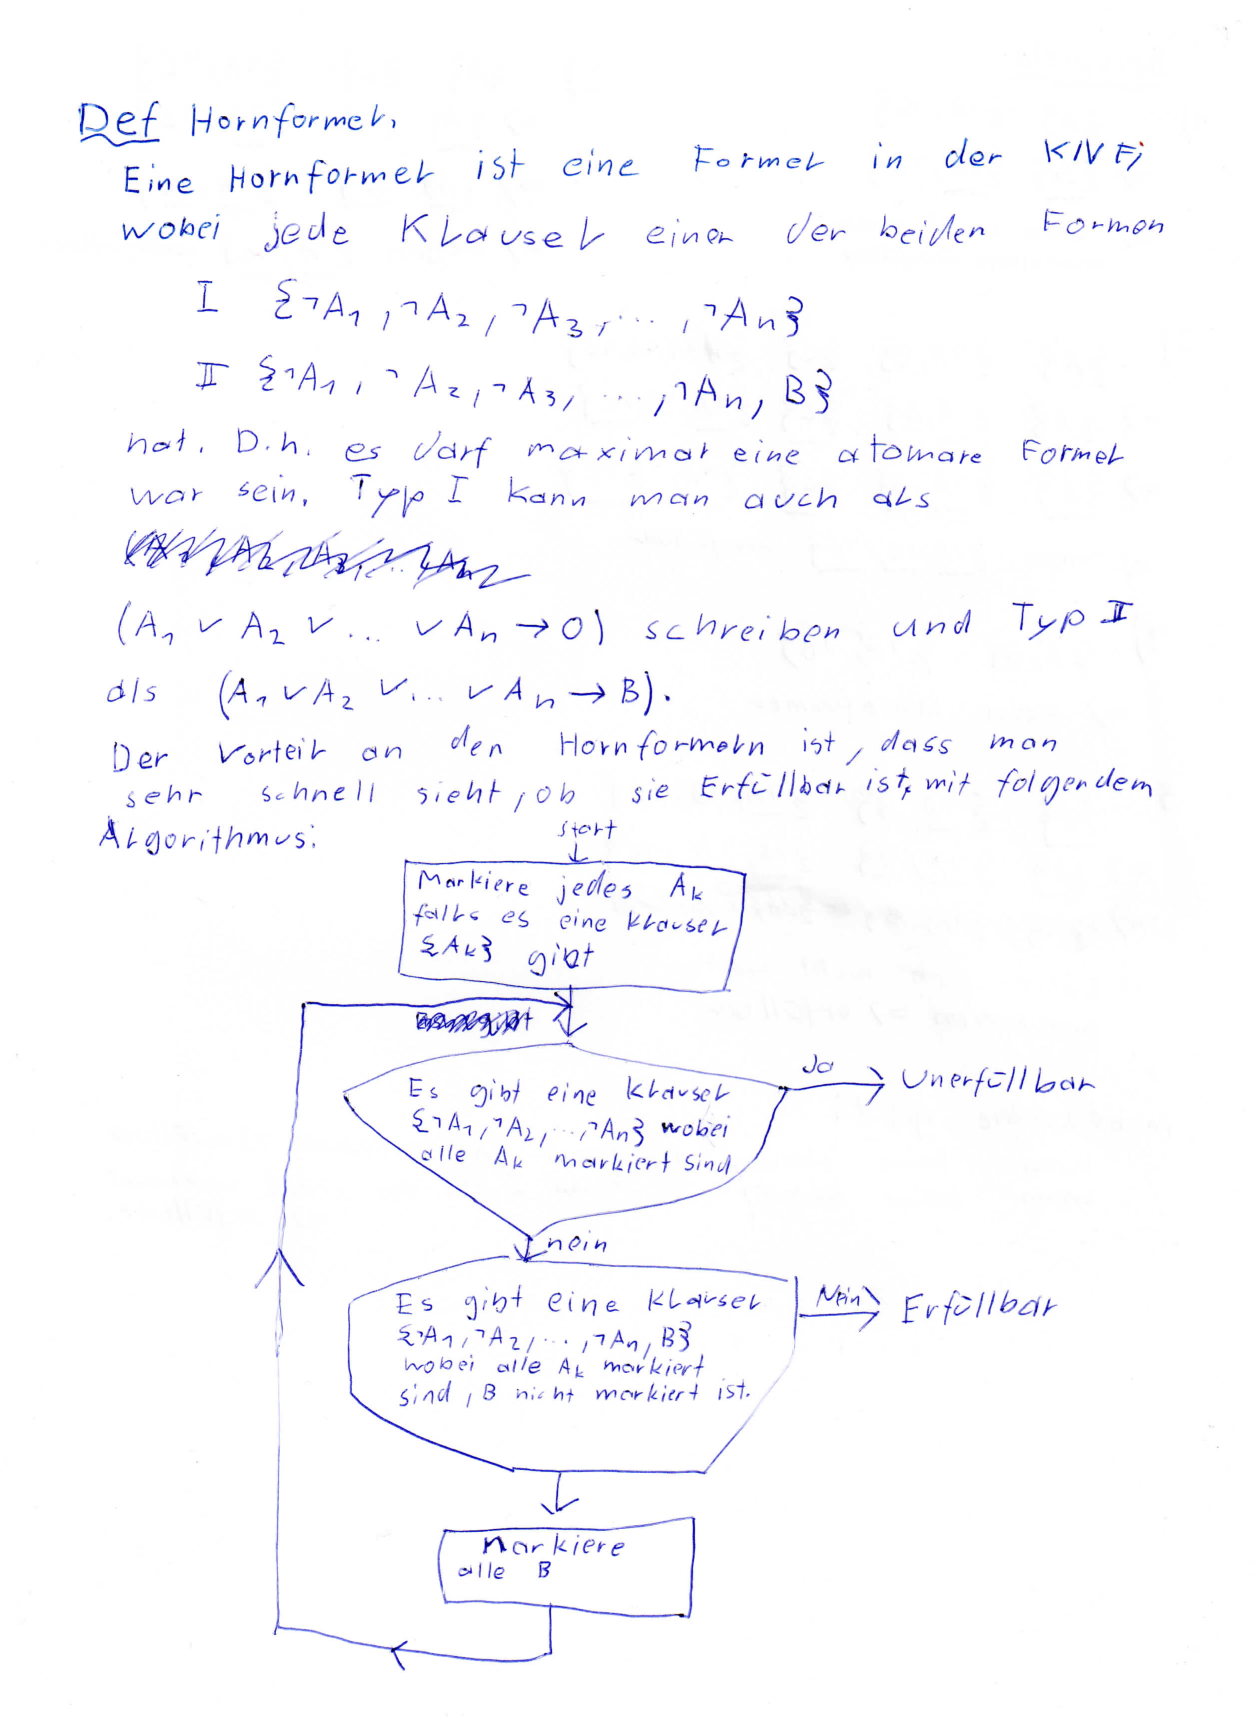
\includepdf{Hornformeln}

\part{Anhänge}
\appendix

%\clearpage
%\phantomsection
%\addcontentsline{toc}{chapter}{Literaturverzeichnis}
%\nocite{*}
%\bibliographystyle{babplain}
%\bibliography{lit}

\end{document}